% ============================================================================
% Báo cáo Seminar: Mobile-U-ViT
% Phân loại lá chè công nghiệp thời gian thực với kiến trúc CNN-Transformer lai
% Biên dịch: pdflatex main.tex (khuyến nghị 2 lần để resolve references)
% Tác giả: Nguyễn Ngọc Bình An, Nguyễn Quang Sang, Nguyễn Đình Phú
% ============================================================================

\documentclass[conference]{IEEEtran}
\usepackage{cite}
\usepackage{amsmath,amssymb,amsfonts}
\usepackage{algorithmic}
\usepackage{graphicx}
\usepackage{textcomp}
\usepackage{xcolor}
\usepackage{booktabs}
\usepackage{multirow}
\usepackage{array}
\usepackage{hyperref}
\usepackage{float}
\usepackage{subcaption}
\usepackage{placeins}
\usepackage{tikz}
\usepackage{adjustbox}
\usetikzlibrary{arrows.meta, positioning, shapes, calc, backgrounds, fit, patterns}
\usepackage[utf8]{vietnam}

% ── Custom math operators ──
\DeclareMathOperator{\softmax}{softmax}
\DeclareMathOperator{\GroupNorm}{GroupNorm}
\DeclareMathOperator{\Sigmoid}{Sigmoid}

\begin{document}

\title{Mobile-U-ViT Hiệu Quả cho Phân Loại\\Lá Chè Công Nghiệp Thời Gian Thực}

\author{
\IEEEauthorblockN{Nguyễn Ngọc Bình An\textsuperscript{1}, Nguyễn Quang Sang\textsuperscript{1}, Nguyễn Đình Phú\textsuperscript{1}}
\IEEEauthorblockA{
\textsuperscript{1}Viện trí tuệ nhân tạo, Trường Đại học Công Nghệ, Đại học Quốc Gia Hà Nội, Việt Nam\\
Email: nguyenan111206@gmail.com}
}

\maketitle

% ============================================================================
% Tóm tắt
% ============================================================================

\begin{abstract}
Phân loại lá chè chính xác và thời gian thực là yếu tố thiết yếu để kiểm soát chất lượng trong ngành công nghiệp chè, tuy nhiên các giải pháp học sâu hiện tại bị hạn chế bởi yêu cầu tính toán cao và phụ thuộc vào lượng lớn dữ liệu được gán nhãn ở cấp độ pixel. Bài báo này trình bày Mobile-U-ViT, một kiến trúc CNN-Transformer lai hiệu quả kết hợp kết nối bỏ qua encoder-decoder kiểu U-Net với self-attention khả phân MobileViTv2 cho phân đoạn ngữ nghĩa công nghiệp. Mô hình giới thiệu bốn biến thể có khả năng mở rộng---Nano (0.3M tham số, $d_{model}=48$), Base (0.6M, $d_{model}=64$), Pro (2.0M, $d_{model}=128$) và ProMax (7.0M, $d_{model}=256$)---cho phép triển khai từ thiết bị biên (Raspberry Pi 5, Jetson Nano) đến máy chủ GPU. Để giải quyết nút thắt về gán nhãn trong lĩnh vực nông nghiệp, chúng tôi tích hợp khung học bán giám sát Mean Teacher và Cross Conv x Transformer tận dụng cả dữ liệu có nhãn và không nhãn. Các thí nghiệm mở rộng trên bộ dữ liệu Bệnh Lá Chè 8 lớp tùy chỉnh cho thấy phương pháp của chúng tôi đạt được độ chính xác phân đoạn cạnh tranh (mIoU \textbf{84.1}\%) với số lượng tham số và FLOPs ít hơn đáng kể so với các phương pháp hiện đại. Hơn nữa, biến thể bán giám sát được huấn luyện chỉ với 10\% dữ liệu có nhãn vẫn giữ được \textbf{85--90}\% hiệu năng so với huấn luyện giám sát hoàn toàn, giảm đáng kể chi phí gán nhãn cho triển khai thực tế. Cài đặt của chúng tôi cho phép suy luận thời gian thực ở \textbf{185.8} FPS (Nano) / \textbf{94.1} FPS (Base) trên thiết bị biên, phù hợp cho đánh giá chất lượng chè tại chỗ trong môi trường hạn chế tài nguyên.
\end{abstract}

\begin{IEEEkeywords}
Mobile-U-ViT, học bán giám sát, phân loại lá chè, phân đoạn ngữ nghĩa, điện toán biên, transformer nhẹ, kiểm soát chất lượng công nghiệp, separable self-attention, MobileNetV2, GroupNorm, Mean Teacher, inverted bottleneck.
\end{IEEEkeywords}

% ============================================================================
% I. INTRODUCTION
% ============================================================================

\section{Giới thiệu}

Chè là một trong những đồ uống được tiêu thụ rộng rãi nhất trên toàn cầu, với sản lượng hàng năm ước tính vượt quá 6 triệu tấn~\cite{b1}. Chất lượng và giá trị thị trường của chè phụ thuộc chủ yếu vào kiểm tra trực quan lá chè đã qua chế biến---một công việc truyền thống do những người phân loại lành nghề thực hiện, phân loại lá dựa trên màu sắc, kết cấu, hình dạng và các khuyết tật nhìn thấy được. Tuy nhiên, quy trình thủ công này gặp phải những thách thức cố hữu: tốn nhiều nhân công, chịu sự biến thiên giữa những người đánh giá, và không thể mở rộng để đáp ứng yêu cầu thông lượng của các cơ sở chế biến chè hiện đại vận hành liên tục.

Thị giác máy tính và học sâu mang lại các giải pháp đầy hứa hẹn cho việc tự động hóa quy trình này. Phân đoạn ngữ nghĩa---phân loại ở cấp độ pixel các vùng lá thành các hạng mục chất lượng---cung cấp thông tin không gian phong phú hơn đáng kể so với phân loại ở cấp độ ảnh và cho phép định vị chính xác các đốm bệnh, sự đổi màu và hư hỏng vật lý trên từng lá riêng lẻ. Những tiến bộ gần đây trong vision transformer (ViT)~\cite{b2} đã thiết lập các kỷ lục mới về hiệu năng phân đoạn nhờ khả năng nắm bắt phụ thuộc tầm xa thông qua cơ chế self-attention. Tuy nhiên, ViT tiêu chuẩn có độ phức tạp bậc hai $\mathcal{O}(N^2)$ theo số lượng token, khiến chúng không phù hợp cho triển khai công nghiệp thời gian thực trên thiết bị biên. Song song với thách thức về hiệu năng tính toán, lĩnh vực nông nghiệp còn đối mặt với vấn đề khan hiếm dữ liệu gán nhãn nghiêm trọng: gán nhãn cấp độ pixel cho lá chè đòi hỏi chuyên môn lĩnh vực và tốn nhiều thời gian, với một ảnh $320 \times 320$ có thể mất 10--20 phút cho một chuyên gia có kinh nghiệm.

Để giải quyết đồng thời cả hai thách thức trên, chúng tôi đề xuất \textbf{Mobile-U-ViT}, một kiến trúc encoder-decoder nhẹ kết hợp hiệp đồng mạng nơ-ron tích chập (CNN) với vision transformer cho phân đoạn ngữ nghĩa hiệu quả. Mobile-U-ViT áp dụng thiết kế kiểu U-Net trong đó mỗi lớp encoder và decoder được xây dựng từ một khối lai ba thành phần: khối cục bộ (tích chập khả phân theo chiều sâu) để trích xuất đặc trưng không gian tinh, khối toàn cục (separable self-attention của MobileViTv2~\cite{b3}) để mô hình hóa ngữ cảnh tầm xa với độ phức tạp tuyến tính $\mathcal{O}(C^2 \cdot P \cdot S)$, và khối mở rộng (inverted bottleneck kiểu MobileNetV2) để làm giàu biểu diễn đặc trưng. Để giảm sự phụ thuộc vào dữ liệu gán nhãn quy mô lớn, chúng tôi tích hợp khung học bán giám sát Mean Teacher~\cite{b4} cho phép mô hình tận dụng hiệu quả lượng lớn ảnh không nhãn sẵn có trong môi trường công nghiệp. Các đóng góp chính của bài báo này bao gồm:

\begin{enumerate}
    \item \textbf{Kiến trúc CNN-Transformer lai với khối UMobileViTLayer thống nhất:} Chúng tôi thiết kế kiến trúc kiểu U-Net trong đó mỗi lớp encoder và decoder được xây dựng từ cùng một khối UMobileViTLayer---tổ hợp tuần tự của ba thành phần: (i) \textit{khối cục bộ} (depthwise $3\times3$ + pointwise $1\times1$ + ReLU + GroupNorm) để trích xuất đặc trưng không gian tinh như cạnh, kết cấu và biến thể màu sắc; (ii) \textit{khối toàn cục} gồm $N$ transformer block với separable self-attention MobileViTv2 hoạt động trên các patch đặc trưng được unfold qua unfold\_custom, đạt độ phức tạp tuyến tính $\mathcal{O}(C^2 \cdot P \cdot S)$ thay vì bậc hai $\mathcal{O}(N^2)$ của self-attention tiêu chuẩn; và (iii) \textit{khối mở rộng} inverted bottleneck kiểu MobileNetV2 (pointwise expand $\rightarrow$ depthwise $3\times3$ $\rightarrow$ pointwise project) với ReLU6 và GroupNorm để ổn định số học và ngăn activation bùng nổ. Mỗi khối được bọc với kết nối residual và GroupNorm đầu ra: $Z = \GroupNorm(X + \text{Expand}(\text{Global}(\text{Local}(X))))$. Trong encoder, transformer sử dụng self-attention; trong decoder, transformer sử dụng cross-attention truy vấn đặc trưng kết nối bỏ qua từ encoder---cho phép hợp nhất có chọn lọc thông tin đa tỷ lệ thay vì concatenate đơn thuần như U-Net truyền thống. Tầng encoder cuối cùng sử dụng patch\_size $(1,1)$, hoạt động như self-attention toàn cục trên toàn bộ bản đồ đặc trưng ở độ phân giải thấp nhất. Tầng decoder đầu ra thay thế cross-attention bằng phép chiếu bộ nhớ cộng tính (\texttt{UMobileViTDecoderConcatLayer}) để giảm FLOPs ở độ phân giải không gian cao.

    \item \textbf{Bốn biến thể có khả năng mở rộng hệ thống với chiến lược mở rộng đồng bộ:} Chúng tôi giới thiệu bốn biến thể---Nano ($d_{model}=48$, $N=1$, $E=2.0$, $\sim$0.3M tham số), Base ($d_{model}=64$, $N=2$, $E=3.0$, $\sim$0.6M), Pro ($d_{model}=128$, $N=3$, $E=3.0$, $\sim$2.0M), và ProMax ($d_{model}=256$, $N=3$, $E=4.0$, $\sim$7.0M)---thu được bằng cách mở rộng đồng bộ ba chiều: chiều đặc trưng cơ sở $d_{model}$, số khối transformer mỗi lớp $N$, và hệ số mở rộng inverted bottleneck $E$. Chiến lược mở rộng này đảm bảo sự cân bằng giữa chiều rộng mạng (qua $d_{model}$), chiều sâu attention (qua $N$), và dung lượng biểu diễn (qua $E$), cho phép phủ toàn bộ phổ triển khai từ thiết bị biên tài nguyên hạn chế (Raspberry Pi 5 CPU-only 8GB, Jetson Nano 128-core Maxwell GPU 4GB) đến máy chủ GPU hiệu năng cao (RTX 3060+), mà không cần thiết kế lại kiến trúc. Điều kiện ràng buộc $d_{model}$ phải chia hết cho 4 (stem), 2 (seg\_head downsampling), và 8 (seg\_head output channels) đảm bảo tính tương thích của toàn bộ pipeline. Hàm \texttt{get\_groupnorm\_groups()} tự động chọn số nhóm GroupNorm tương thích khi số kênh không chia hết cho target groups, loại bỏ nhu cầu điều chỉnh thủ công.

    \item \textbf{Khung học bán giám sát Mean Teacher cải tiến với hai DataLoader không nhãn:} Chúng tôi tích hợp thuật toán Mean Teacher~\cite{b4} để tận dụng ảnh lá chè không nhãn thông qua ràng buộc nhất quán, với ba cải tiến then chốt so với cài đặt tiêu chuẩn. \textit{Thứ nhất}, thay vì dùng một DataLoader không nhãn với hai lần lan truyền xuôi (student có gradient, teacher không gradient), chúng tôi xây dựng \textbf{hai DataLoader không nhãn riêng biệt} từ cùng tập con nhưng với seed shuffle khác nhau---đảm bảo student và teacher quan sát các phép tăng cường \textit{khác nhau} trên mỗi ảnh, tối đa hóa đa dạng nhiễu cho consistency regularization. \textit{Thứ hai}, teacher được cập nhật qua EMA ($\alpha=0.999$) sau \textbf{mỗi bước tối ưu} (không chỉ ở biên epoch), cung cấp tín hiệu nhất quán liên tục và cho phép teacher theo sát student trong suốt quá trình huấn luyện. \textit{Thứ ba}, validation sử dụng teacher model (vốn có hiệu năng cao hơn student nhờ weight averaging), phản ánh chính xác hơn chất lượng mô hình sẽ được triển khai. Hàm loss nhất quán sử dụng MSE giữa softmax của student và teacher, với trọng số $\lambda(t)$ tuân theo lịch trình sigmoid ramp-up trong 50 epoch đầu để tránh teacher chưa ổn định tạo mục tiêu nhiễu. Hàm loss giám sát kết hợp Cross-Entropy (với trọng số lớp nghịch đảo tần suất và label smoothing $\epsilon=0.1$) và Dice loss theo tỷ lệ 50/50 để xử lý mất cân bằng lớp.

    \item \textbf{Tiêu chuẩn đánh giá toàn diện trên bài toán phân loại lá chè công nghiệp:} Chúng tôi xây dựng bộ dữ liệu phân loại chất lượng và bệnh lá chè 8 lớp (Healthy Leaf, Brown Blight, Algal Spot, Bird's Eye Spot, Gray Blight, Red Rust, Leaf Miner Damage, Background/Other) từ 10,000 mẫu được gán nhãn ở độ phân giải $320 \times 320$. Chúng tôi thực hiện đánh giá có hệ thống bao gồm: (i) so sánh với các phương pháp phân đoạn hiện đại (U-Net, DeepLabV3+, SegFormer, LR-ASPP) trên các chỉ số mIoU, Pixel Accuracy, Dice Coefficient, tham số, FLOPs và độ trễ suy luận; (ii) nghiên cứu cắt bỏ (ablation) từng thành phần kiến trúc---khối toàn cục (transformer attention), khối mở rộng (inverted bottleneck), cross-attention decoder, Feature Refinement Block, GroupNorm vs BatchNorm, và gradient checkpointing; (iii) phân tích hiệu năng bán giám sát ở các tỷ lệ dữ liệu có nhãn khác nhau (10\%, 25\%, 50\%, 100\%) với so sánh giữa chế độ giám sát hoàn toàn, bán giám sát Mean Teacher, và chỉ giám sát trên tập con; (iv) đo lường độ trễ suy luận thực tế trên bốn nền tảng biên (Jetson Nano 4GB, Jetson Xavier NX, Jetson Orin Nano, Raspberry Pi 5) ở định dạng FP32; và (v) phân tích trực quan bao gồm bản đồ nhiệt kích hoạt theo từng tầng (layer-wise activation heatmap), ma trận nhầm lẫn theo lớp, và phân phối lỗi để hiểu cơ chế hoạt động nội tại của mô hình.
\end{enumerate}

Phần còn lại của bài báo được tổ chức như sau. Mục~II điểm lại các công trình liên quan về phân đoạn ngữ nghĩa nhẹ, vision transformer cho thiết bị di động, học bán giám sát cho phân đoạn, và đánh giá chất lượng lá chè. Mục~III trình bày chi tiết kiến trúc Mobile-U-ViT bao gồm stem, khối UMobileViTLayer (local, global transformer với separable attention, expansion inverted bottleneck, residual connection), thiết kế encoder và decoder (với cross-attention và additive memory projection), đầu phân đoạn (UpsampleHead, FeatureRefinementBlock, bộ phân loại nhẹ, MultiTaskDenseHead), bảng cấu hình bốn biến thể, và chiến lược ổn định số học. Mục~IV mô tả khung học bán giám sát Mean Teacher với phát biểu bài toán, kiến trúc student-teacher, hàm mục tiêu kết hợp (supervised CE + Dice và unsupervised consistency MSE), lịch trình sigmoid ramp-up, pipeline tăng cường dữ liệu ba mức cường độ (Light/Medium/Strong), thuật toán huấn luyện chi tiết, và chiến lược quản lý bộ nhớ. Mục~V trình bày thiết lập thí nghiệm bao gồm bộ dữ liệu, cấu hình huấn luyện, các chỉ số đánh giá, nền tảng phần cứng, và các phương pháp cơ sở. Mục~VI thảo luận kết quả và phân tích. Mục~VII kết luận và đề xuất hướng nghiên cứu tiếp theo.

% ============================================================================
% II. RELATED WORK
% ============================================================================

\section{Công trình Liên quan}

\subsection{Phân đoạn ngữ nghĩa nhẹ}

Kiến trúc encoder-decoder đã trở thành nền tảng cho phân đoạn ngữ nghĩa kể từ U-Net~\cite{b5}, với kết nối bỏ qua (skip connection) đóng vai trò then chốt trong việc bảo toàn chi tiết không gian mịn qua các tầng giảm độ phân giải. Tuy nhiên, triển khai các kiến trúc này trên thiết bị biên đòi hỏi sự đánh đổi cẩn thận giữa độ chính xác và chi phí tính toán.

MobileNetV2~\cite{b6} thiết lập mô hình thiết kế cho mạng tích chập hiệu quả thông qua inverted bottleneck với tích chập khả phân chiều sâu (depthwise separable convolution). Ý tưởng cốt lõi là phân rã tích chập tiêu chuẩn $\mathbb{R}^{K \times K \times C_{\text{in}} \times C_{\text{out}}}$ thành hai phép toán rẻ hơn: depthwise $K \times K \times C$ (xử lý từng kênh độc lập) và pointwise $1 \times 1 \times C \times C_{\text{out}}$ (trộn thông tin liên kênh), giảm một bậc độ lớn cả tham số lẫn FLOPs. DeepLabV3+~\cite{b7} kết hợp atrous spatial pyramid pooling (ASPP) với một bộ giải mã nhẹ để khôi phục chi tiết biên, chứng minh rằng một bộ mã hóa nặng có thể được bổ trợ bởi một bộ giải mã đơn giản. LR-ASPP~\cite{b19} đẩy xa hơn triết lý này, rút gọn ASPP thành thiết kế tối giản dựa trên MobileNetV3 nhắm đến suy luận thời gian thực. SegFormer~\cite{b8} thay thế hoàn toàn bộ mã hóa tích chập bằng transformer phân cấp, nhưng self-attention tiêu chuẩn trong bộ mã hóa vẫn giữ độ phức tạp bậc hai $\mathcal{O}(N^2)$, hạn chế khả năng mở rộng lên ảnh độ phân giải cao.

Một hạn chế chung của các phương pháp trên là sự bất đối xứng giữa encoder và decoder: cơ chế attention---nếu có---thường chỉ tập trung trong encoder, trong khi decoder vẫn là các phép tích chập hoặc MLP đơn giản. Điều này bỏ lỡ cơ hội khai thác attention cho việc hợp nhất có chọn lọc thông tin đa tỷ lệ trong decoder.

\subsection{Vision Transformer cho thiết bị di động}

Vision Transformer (ViT)~\cite{b2} đã chứng minh rằng kiến trúc transformer thuần túy có thể cạnh tranh với CNN trong thị giác máy tính, nhưng chi phí self-attention $\mathcal{O}(N^2)$ cản trở ứng dụng thực tế trên thiết bị hạn chế tài nguyên. Nhiều nỗ lực đã tìm cách giảm độ phức tạp này trong khi duy trì khả năng mô hình hóa toàn cục.

MobileViT~\cite{b9} là một trong những thiết kế đầu tiên kết hợp thành công CNN và transformer trong một kiến trúc nhẹ: các khối MobileNetV2 trích xuất đặc trưng cục bộ, trong khi các khối transformer hoạt động trên các patch đặc trưng đã unfold để nắm bắt phụ thuộc tầm xa. MobileViTv2~\cite{b3} cải tiến đáng kể hiệu quả thông qua \textit{separable self-attention}---thay vì tính attention score trên chiều không gian ($S \times S$), phép toán được thực hiện trên chiều kênh ($C \times C$), giảm độ phức tạp xuống $\mathcal{O}(C^2 \cdot P \cdot S)$, tuyến tính theo số lượng patch. Mobile-Former~\cite{b10} khám phá một hướng khác: duy trì hai nhánh CNN và transformer song song, hợp nhất thông tin qua cross-attention hai chiều ở mỗi tầng.

Mặc dù hiệu quả, các kiến trúc trên được thiết kế chủ yếu cho phân loại ảnh. Việc mở rộng chúng sang phân đoạn ngữ nghĩa---bài toán yêu cầu dự đoán dày đặc ở cấp độ pixel---đặt ra những thách thức riêng: (1) làm thế nào để nhúng attention vào cả encoder \textit{và} decoder một cách nhất quán; (2) làm thế nào để decoder khai thác attention cho việc hợp nhất đặc trưng đa tỷ lệ từ encoder; và (3) làm thế nào để duy trì chi phí tuyến tính ở các tầng có độ phân giải cao.

\subsection{Học bán giám sát cho phân đoạn}

Học bán giám sát (SSL) giải quyết bài toán khan hiếm dữ liệu gán nhãn bằng cách tận dụng lượng lớn dữ liệu không nhãn. Trong số các hướng tiếp cận, \textit{consistency regularization}---thực thi tính bất biến của dự đoán dưới các nhiễu đầu vào khác nhau---đã chứng minh hiệu quả vượt trội.

Các phương pháp consistency đời đầu như $\Pi$-Model và Temporal Ensembling~\cite{b11} thiết lập nền tảng: $\Pi$-Model phạt sự khác biệt giữa hai lần lan truyền xuôi với dropout và tăng cường ngẫu nhiên khác nhau; Temporal Ensembling duy trì trung bình trượt hàm mũ (EMA) của các dự đoán làm mục tiêu ổn định hơn. Mean Teacher~\cite{b4} cải tiến đáng kể bằng cách áp dụng EMA lên \textit{trọng số mô hình} thay vì dự đoán, tạo ra một ``giáo viên'' có chất lượng cao hơn và ổn định hơn học sinh---đặc biệt quan trọng khi tập có nhãn rất nhỏ.

Trong phân đoạn ngữ nghĩa, bài toán consistency phức tạp hơn do đầu ra là bản đồ pixel thay vì vector lớp. CutMix~\cite{b12} và ClassMix~\cite{b14} mở rộng không gian nhiễu bằng cách trộn các vùng ảnh từ các mẫu có nhãn và không nhãn. FixMatch~\cite{b13} kết hợp tăng cường yếu-mạnh với ngưỡng tin cậy để tạo pseudo-label, đạt kết quả ấn tượng nhưng yêu cầu cài đặt cẩn thận ngưỡng và tỷ lệ dữ liệu. CPS~\cite{b15} thực thi giám sát chéo giả giữa hai mạng được khởi tạo độc lập, đánh đổi chi phí tính toán gấp đôi để có hiệu năng cao hơn.

Một vấn đề ít được thảo luận trong các công trình trên là \textit{chất lượng và tần suất cập nhật} của teacher trong quá trình huấn luyện. Hầu hết các cài đặt cập nhật teacher ở biên epoch, bỏ lỡ cơ hội cung cấp tín hiệu nhất quán liên tục cho student.

\subsection{Đánh giá chất lượng lá chè}

Các nghiên cứu về tự động hóa đánh giá chất lượng chè chủ yếu dừng ở phân loại cấp độ ảnh: học máy truyền thống với đặc trưng thủ công~\cite{b16} hoặc CNN tiêu chuẩn~\cite{b17} phân loại từng lá thành các hạng chất lượng. Một số công trình gần đây khám phá phát hiện đối tượng cho bệnh lá~\cite{b18}, nhưng phân đoạn ngữ nghĩa cấp độ pixel cho phân loại chất lượng toàn diện---phân định chính xác từng vùng bệnh, khuyết tật, và biến thể màu sắc trên bề mặt lá---vẫn là một khoảng trống nghiên cứu.

Thách thức đặc thù của bài toán này bao gồm: (1) ranh giới mờ giữa các loại khuyết tật (đốm nâu, đốm tảo, vết rỉ sắt có hình thái chồng lấp); (2) kích thước tổn thương đa dạng từ vài pixel (vết côn trùng) đến vùng lớn (cháy lá); và (3) yêu cầu suy luận thời gian thực trên thiết bị biên trong môi trường nhà máy. Những thách thức này đòi hỏi một kiến trúc vừa có khả năng mô hình hóa ngữ cảnh tầm xa (để phân biệt các lớp có hình thái tương tự), vừa bảo toàn chi tiết không gian mịn (để phát hiện tổn thương nhỏ), vừa đủ nhẹ để chạy trên thiết bị biên.

% ============================================================================
% III. METHODOLOGY
% ============================================================================

\section{Kiến trúc Mobile-U-ViT}

\subsection{Tổng quan Thiết kế}

Mobile-U-ViT là một kiến trúc encoder-decoder phân cấp, được tối ưu hóa cho bài toán phân đoạn ngữ nghĩa trên thiết bị biên. Triết lý thiết kế cốt lõi của mô hình là \textbf{nhúng cơ chế attention một cách nhất quán} ở cả bộ mã hóa (encoder) lẫn bộ giải mã (decoder), khắc phục hạn chế của các mạng U-Net truyền thống vốn chỉ dùng tích chập đơn giản ở decoder.

Hình~\ref{fig:architecture} minh họa 4 thành phần chính của kiến trúc:

\begin{itemize}
    \item \textbf{Stem (Khối gốc):} Gồm 3 tầng tích chập giúp giảm nhanh độ phân giải không gian xuống 8 lần ($H/8 \times W/8$) và tăng số lượng kênh để tạo đặc trưng ban đầu.
    \item \textbf{Encoder (Bộ mã hóa):} Gồm 3 stage. Mỗi stage thực hiện giảm kích thước (downsample) 2 lần và áp dụng self-attention để trích xuất đặc trưng ngữ cảnh từ cục bộ đến toàn cục.
    \item \textbf{Decoder (Bộ giải mã):} Đối xứng với encoder. Đặc biệt, nó sử dụng \textit{cross-attention} để chắt lọc thông tin hữu ích từ các kết nối bỏ qua (skip connections) thay vì chỉ nối (concatenate) một cách thụ động.
    \item \textbf{Segmentation Head (Đầu phân đoạn):} Phục hồi lại độ phân giải gốc qua 3 bước upsampling, làm mịn đường biên bằng dilated convolution \& spatial attention, trước khi phân loại từng pixel.
\end{itemize}

\begin{figure}[t]
\centering
\adjustbox{max width=\columnwidth}{% ============================================================================
% Kiến trúc tổng quát Mobile-U-ViT — TikZ diagram
% Biên dịch: pdflatex (cần package tikz)
% ============================================================================
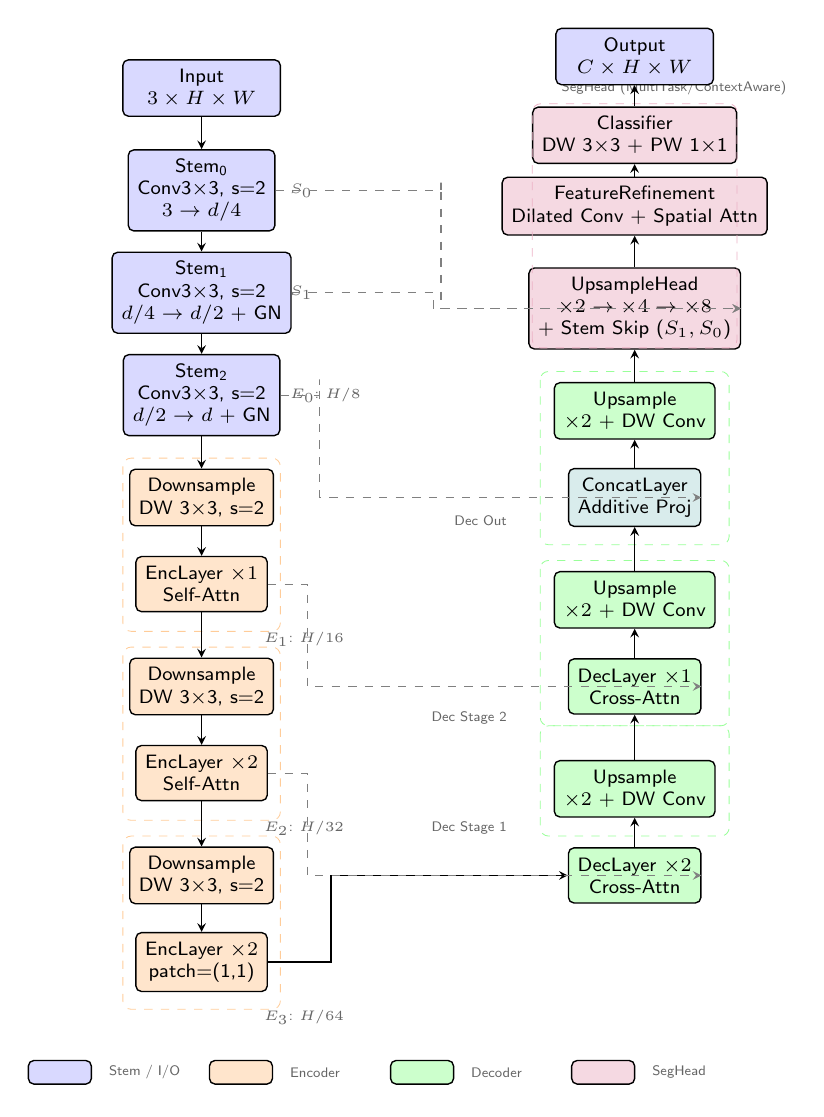
\begin{tikzpicture}[
    % ── Style definitions ──
    block/.style={
        rectangle, draw=black, line width=0.5pt,
        minimum width=1.6cm, minimum height=0.55cm,
        align=center, font=\scriptsize\sffamily,
        rounded corners=2pt,
    },
    stem/.style={block, fill=blue!15},
    enc/.style={block, fill=orange!20},
    dec/.style={block, fill=green!20},
    head/.style={block, fill=purple!15},
    attn/.style={block, fill=red!10},
    concat/.style={block, fill=teal!15},
    arrow/.style={->, >=stealth, line width=0.4pt},
    skip/.style={->, >=stealth, line width=0.4pt, dashed, gray},
    box/.style={rectangle, draw=black!40, line width=0.3pt, dashed, rounded corners=3pt},
    lbl/.style={font=\tiny\sffamily, text=black!60},
]

% ═══════════════════════════════════════════════════════════════
% INPUT
% ═══════════════════════════════════════════════════════════════
\node[stem, minimum width=2.0cm] (input) at (0, 10.5) {Input\\$3 \times H \times W$};

% ═══════════════════════════════════════════════════════════════
% STEM (3 tầng)
% ═══════════════════════════════════════════════════════════════
\node[stem] (stem0) at (0, 9.2) {Stem\textsubscript{0}\\Conv3$\times$3, s=2\\$3\to d/4$};
\node[stem] (stem1) at (0, 7.9) {Stem\textsubscript{1}\\Conv3$\times$3, s=2\\$d/4\to d/2$ + GN};
\node[stem] (stem2) at (0, 6.6) {Stem\textsubscript{2}\\Conv3$\times$3, s=2\\$d/2\to d$ + GN};

% Stem outputs annotation
\node[lbl, anchor=west] at (1.0, 9.2) {$S_0$};
\node[lbl, anchor=west] at (1.0, 7.9) {$S_1$};

% ═══════════════════════════════════════════════════════════════
% ENCODER (3 stage)
% ═══════════════════════════════════════════════════════════════
% Stage 1
\node[enc] (enc1_ds) at (0, 5.3) {Downsample\\DW 3$\times$3, s=2};
\node[enc, minimum height=0.7cm] (enc1_l) at (0, 4.2) {EncLayer $\times 1$\\Self-Attn};

% Stage 2
\node[enc] (enc2_ds) at (0, 2.9) {Downsample\\DW 3$\times$3, s=2};
\node[enc, minimum height=0.7cm] (enc2_l) at (0, 1.8) {EncLayer $\times 2$\\Self-Attn};

% Stage 3
\node[enc] (enc3_ds) at (0, 0.5) {Downsample\\DW 3$\times$3, s=2};
\node[enc, minimum height=0.7cm] (enc3_l) at (0, -0.6) {EncLayer $\times 2$\\patch=(1,1)};

% Encoder stage boxes
\draw[box, orange!40] (-1.0, 5.8) rectangle (1.0, 3.6);
\node[lbl] at (1.3, 3.5) {$E_1$: $H/16$};

\draw[box, orange!40] (-1.0, 3.4) rectangle (1.0, 1.2);
\node[lbl] at (1.3, 1.1) {$E_2$: $H/32$};

\draw[box, orange!40] (-1.0, 1.0) rectangle (1.0, -1.2);
\node[lbl] at (1.3, -1.3) {$E_3$: $H/64$};

% Encoder annotations
\node[lbl, anchor=west] at (1.0, 6.6) {$E_0$: $H/8$};

% ═══════════════════════════════════════════════════════════════
% DECODER (3 stage) — bên phải, mirror encoder
% ═══════════════════════════════════════════════════════════════

% Stage 1 (decoder) — xử lý từ dưới lên
\node[dec, minimum height=0.7cm] (dec1_l) at (5.5, 0.5) {DecLayer $\times 2$\\Cross-Attn};
\node[dec] (dec1_us) at (5.5, 1.6) {Upsample\\$\times 2$ + DW Conv};

% Stage 2
\node[dec, minimum height=0.7cm] (dec2_l) at (5.5, 2.9) {DecLayer $\times 1$\\Cross-Attn};
\node[dec] (dec2_us) at (5.5, 4.0) {Upsample\\$\times 2$ + DW Conv};

% Out block
\node[concat, minimum height=0.7cm] (dec3_l) at (5.5, 5.3) {ConcatLayer\\Additive Proj};
\node[dec] (dec3_us) at (5.5, 6.4) {Upsample\\$\times 2$ + DW Conv};

% Decoder stage boxes
\draw[box, green!40] (4.3, 2.4) rectangle (6.7, 1.0);
\node[lbl, anchor=east] at (4.0, 1.1) {Dec Stage 1};

\draw[box, green!40] (4.3, 4.5) rectangle (6.7, 2.4);
\node[lbl, anchor=east] at (4.0, 2.5) {Dec Stage 2};

\draw[box, green!40] (4.3, 6.9) rectangle (6.7, 4.7);
\node[lbl, anchor=east] at (4.0, 5.0) {Dec Out};

% ═══════════════════════════════════════════════════════════════
% SEG HEAD
% ═══════════════════════════════════════════════════════════════
\node[head] (seg_us) at (5.5, 7.7) {UpsampleHead\\$\times 2 \to \times 4 \to \times 8$\\+ Stem Skip ($S_1,S_0$)};
\node[head, minimum height=0.7cm] (seg_ref) at (5.5, 9.0) {FeatureRefinement\\Dilated Conv + Spatial Attn};
\node[head, minimum height=0.6cm] (seg_cls) at (5.5, 9.9) {Classifier\\DW 3$\times$3 + PW 1$\times$1};

\draw[box, purple!30] (4.2, 7.2) rectangle (6.8, 10.3);
\node[lbl] at (6.0, 10.5) {SegHead (MultiTask/ContextAware)};

% Output
\node[stem, minimum width=2.0cm] (output) at (5.5, 10.9) {Output\\$C \times H \times W$};

% ═══════════════════════════════════════════════════════════════
% ARROWS — Main forward path
% ═══════════════════════════════════════════════════════════════

% Input → Stem
\draw[arrow] (input) -- (stem0);
\draw[arrow] (stem0) -- (stem1);
\draw[arrow] (stem1) -- (stem2);

% Stem → Encoder
\draw[arrow] (stem2) -- (enc1_ds);
\draw[arrow] (enc1_ds) -- (enc1_l);
\draw[arrow] (enc1_l) -- (enc2_ds);
\draw[arrow] (enc2_ds) -- (enc2_l);
\draw[arrow] (enc2_l) -- (enc3_ds);
\draw[arrow] (enc3_ds) -- (enc3_l);

% Latent → Decoder (bottom connection)
\draw[arrow] (enc3_l.east) -- ++(0.8, 0) |- (dec1_l.west);

% Decoder upward
\draw[arrow] (dec1_l) -- (dec1_us);
\draw[arrow] (dec1_us) -- (dec2_l);
\draw[arrow] (dec2_l) -- (dec2_us);
\draw[arrow] (dec2_us) -- (dec3_l);
\draw[arrow] (dec3_l) -- (dec3_us);

% Decoder → SegHead
\draw[arrow] (dec3_us) -- (seg_us);
\draw[arrow] (seg_us) -- (seg_ref);
\draw[arrow] (seg_ref) -- (seg_cls);
\draw[arrow] (seg_cls) -- (output);

% ═══════════════════════════════════════════════════════════════
% SKIP CONNECTIONS (Encoder → Decoder)
% ═══════════════════════════════════════════════════════════════

% E_2 → Dec Stage 1 (cross-attention memory)
\draw[skip] (enc2_l.east) -- ++(0.5, 0) -- ++(0, -0.5) |- (dec1_l.east);

% E_1 → Dec Stage 2 (cross-attention memory)
\draw[skip] (enc1_l.east) -- ++(0.5, 0) -- ++(0, -0.5) |- (dec2_l.east);

% E_0 → Dec Out (ConcatLayer memory)
\draw[skip] (stem2.east) -- ++(0.5, 0) -- ++(0, +0.2) |- (dec3_l.east);

% ═══════════════════════════════════════════════════════════════
% STEM SKIPS (Stem → UpsampleHead)
% ═══════════════════════════════════════════════════════════════
\draw[skip] (stem1.east) -- ++(1.8, 0) -- ++(0, -0.1) |- (seg_us.east);
\draw[skip] (stem0.east) -- ++(2.1, 0) -- ++(0, +0.1) |- (seg_us.east);

% ═══════════════════════════════════════════════════════════════
% LEGEND
% ═══════════════════════════════════════════════════════════════
\node[stem, minimum width=0.8cm, minimum height=0.3cm, font=\tiny] at (-1.8, -2.0) {};
\node[lbl, anchor=west] at (-1.3, -2.0) {Stem / I/O};
\node[enc, minimum width=0.8cm, minimum height=0.3cm, font=\tiny] at (0.5, -2.0) {};
\node[lbl, anchor=west] at (1.0, -2.0) {Encoder};
\node[dec, minimum width=0.8cm, minimum height=0.3cm, font=\tiny] at (2.8, -2.0) {};
\node[lbl, anchor=west] at (3.3, -2.0) {Decoder};
\node[head, minimum width=0.8cm, minimum height=0.3cm, font=\tiny] at (5.1, -2.0) {};
\node[lbl, anchor=west] at (5.6, -2.0) {SegHead};

\end{tikzpicture}
}
\caption{\textbf{Tổng quan kiến trúc Mobile-U-ViT.} Sơ đồ hiển thị luồng dữ liệu end-to-end: Input $\rightarrow$ Stem (3 tầng Conv+ReLU+GN giảm dần độ phân giải $H \rightarrow H/2 \rightarrow H/4 \rightarrow H/8$) $\rightarrow$ Encoder (3 stage với MobileViT encoder layers---mỗi stage downsample 2$\times$ và áp dụng self-attention) $\rightarrow$ Decoder (3 stage đối xứng---upsample 2$\times$ và dùng cross-attention để truy vấn skip connections từ encoder) $\rightarrow$ SegHead (3 bước upsample $\times$2 + Feature Refinement + Pixel Classifier). Các đường nét đứt là skip connections; decoder dùng cross-attention thay vì concat đơn thuần như U-Net truyền thống.}
\label{fig:architecture}
\end{figure}

Luồng dữ liệu tổng quát có thể tóm tắt như sau:
\begin{equation}
\begin{aligned}
\text{Input} &\xrightarrow{\text{Stem}} (S_0, S_1, E_0) \\
E_0 &\xrightarrow{\text{Encoder}} (E_1, E_2, E_3) \\
(E_3, E_2, E_1, E_0) &\xrightarrow{\text{Decoder}} D_{\text{out}} \\
(D_{\text{out}}, S_1, S_0) &\xrightarrow{\text{SegHead}} \text{Output}
\end{aligned}
\end{equation}

% ---------------------------------------------------------
\subsection{Khối Stem (Tiền xử lý)}

Khối Stem đóng vai trò "mở đường", chuyển đổi ảnh RGB thành các biểu diễn không gian có ý nghĩa trước khi đưa vào Transformer. Khối này sử dụng 3 tầng Convolution $3\times3$ (stride=2), kết hợp với ReLU và GroupNorm:

\begin{itemize}
    \item $\mathbf{S_0}$ (giảm $2\times$): Giữ lại làm skip connection số 1.
    \item $\mathbf{S_1}$ (giảm $4\times$): Giữ lại làm skip connection số 2.
    \item $\mathbf{E_0}$ (giảm $8\times$): Đầu vào chính cho Encoder và skip connection cuối cho Decoder.
\end{itemize}

\begin{table}[t]
\centering
\caption{Cấu hình số kênh của khối Stem theo từng biến thể}
\label{tab:stem_channels}
\begin{tabular}{l|c|c|c}
\toprule
\textbf{Biến thể} & $\mathbf{S_0}$ (Res $H/2$) & $\mathbf{S_1}$ (Res $H/4$) & $\mathbf{E_0}$ (Res $H/8$) \\
\midrule
Nano   & 12  & 24  & 48 \\
Base   & 16  & 32  & 64 \\
Pro    & 32  & 64  & 128 \\
ProMax & 64  & 128 & 256 \\
\bottomrule
\end{tabular}
\end{table}

% ---------------------------------------------------------
\subsection{Trái tim của mô hình: Khối UMobileViTLayer}

Thay vì tách biệt thiết kế CNN và Transformer, Mobile-U-ViT sử dụng một khối thống nhất duy nhất (UMobileViTLayer) cho mọi lớp. Khối này là một đường ống (pipeline) đi qua 3 bước, được bọc bởi kết nối residual (Hình~\ref{fig:umobilevit_layer}):

\begin{enumerate}
    \item \textbf{Local Block (Đặc trưng cục bộ):} Sử dụng Depthwise + Pointwise Convolution để nắm bắt các chi tiết mịn như cạnh, màu sắc. (Độ phức tạp $\mathcal{O}(C \cdot H \cdot W)$).
    
    \item \textbf{Global Block (Ngữ cảnh tầm xa):} Đây là nơi Transformer hoạt động. Để giảm chi phí tính toán, nó áp dụng các bước:
    \begin{itemize}
        \item \textit{Unfold:} Chia ảnh thành các patch nhỏ không chồng lấn.
        \item \textit{Separable Attention:} Tính attention trên chiều \textit{kênh} thay vì chiều không gian, giảm độ phức tạp từ bình phương xuống tuyến tính $\mathcal{O}(C^2 \cdot P \cdot S)$.
        \item \textit{Fold:} Ghép các patch lại thành ảnh 2D ban đầu.
    \end{itemize}
    
    \item \textbf{Expansion Block (Làm giàu biểu diễn):} Hoạt động như một Inverted Bottleneck (tương tự MobileNetV2), mở rộng số kênh lên $E$ lần (từ 2 đến 4 lần) để mô hình học được các đặc trưng phức tạp hơn, sau đó thu hẹp lại.
\end{enumerate}

\begin{figure}[t]
\centering
\adjustbox{max width=\columnwidth}{% ============================================================================
% Chi tiết khối _UMobileViTLayer — TikZ diagram
% ============================================================================
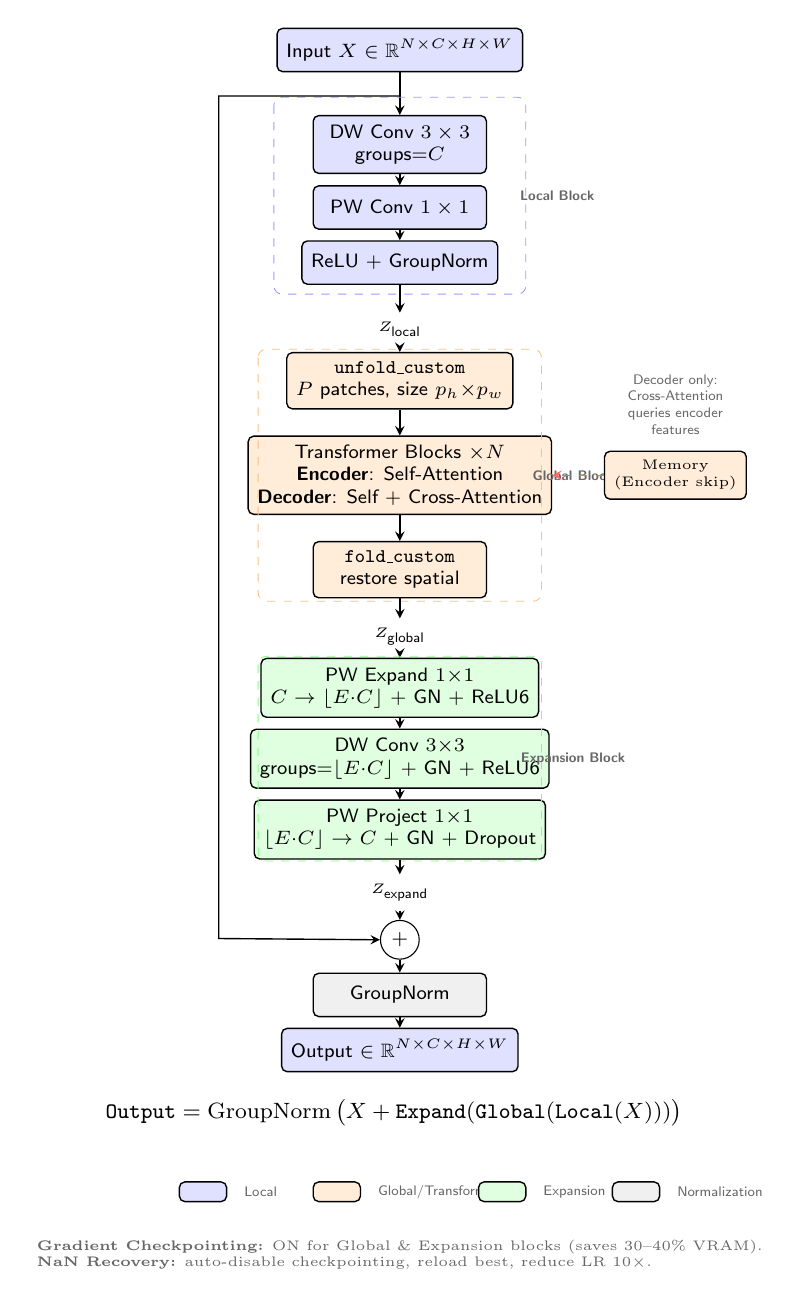
\begin{tikzpicture}[
    block/.style={
        rectangle, draw=black, line width=0.5pt,
        minimum width=2.2cm, minimum height=0.55cm,
        align=center, font=\scriptsize\sffamily,
        rounded corners=2pt,
    },
    local/.style={block, fill=blue!12},
    global/.style={block, fill=orange!15},
    expand/.style={block, fill=green!12},
    norm/.style={block, fill=gray!12},
    arrow/.style={->, >=stealth, line width=0.5pt},
    plus/.style={circle, draw=black, fill=white, inner sep=0pt, minimum size=14pt, font=\scriptsize},
    box/.style={rectangle, draw=black!40, line width=0.3pt, dashed, rounded corners=3pt},
    lbl/.style={font=\tiny\sffamily, text=black!60},
]

% INPUT
\node[local, minimum width=2.8cm] (input) at (0, 0) {Input $X \in \mathbb{R}^{N \times C \times H \times W}$};

% LOCAL BLOCK
\node[local] (dw) at (0, -1.2) {DW Conv $3\times3$\\groups=$C$};
\node[local] (pw1) at (0, -2.0) {PW Conv $1\times1$};
\node[local] (act1) at (0, -2.7) {ReLU + GroupNorm};

\draw[arrow] (input) -- (dw);
\draw[arrow] (dw) -- (pw1);
\draw[arrow] (pw1) -- (act1);

\draw[box, blue!40] (-1.6, -0.6) rectangle (1.6, -3.1);
\node[lbl] at (2.0, -1.85) {\textbf{Local Block}};

\node[font=\tiny\sffamily] (lout) at (0, -3.55) {$Z_{\text{local}}$};
\draw[arrow] (act1) -- (lout);

% GLOBAL BLOCK
\node[global] (unfold) at (0, -4.2) {\texttt{unfold\_custom}\\$P$ patches, size $p_h{\times}p_w$};
\node[global, minimum height=0.8cm] (trans) at (0, -5.4) {Transformer Blocks $\times N$\\\textbf{Encoder}: Self-Attention\\\textbf{Decoder}: Self + Cross-Attention};
\node[global] (fold) at (0, -6.6) {\texttt{fold\_custom}\\restore spatial};

\draw[arrow] (lout) -- (unfold);
\draw[arrow] (unfold) -- (trans);
\draw[arrow] (trans) -- (fold);

\draw[box, orange!50] (-1.8, -3.8) rectangle (1.8, -7.0);
\node[lbl] at (2.2, -5.4) {\textbf{Global Block}};

\node[font=\tiny\sffamily] (gout) at (0, -7.45) {$Z_{\text{global}}$};
\draw[arrow] (fold) -- (gout);

% EXPANSION BLOCK
\node[expand] (exp_pw) at (0, -8.1) {PW Expand $1{\times}1$\\$C \to \lfloor E{\cdot}C\rfloor$ + GN + ReLU6};
\node[expand] (exp_dw) at (0, -9.0) {DW Conv $3{\times}3$\\groups=$\lfloor E{\cdot}C\rfloor$ + GN + ReLU6};
\node[expand] (exp_proj) at (0, -9.9) {PW Project $1{\times}1$\\$\lfloor E{\cdot}C\rfloor \to C$ + GN + Dropout};

\draw[arrow] (gout) -- (exp_pw);
\draw[arrow] (exp_pw) -- (exp_dw);
\draw[arrow] (exp_dw) -- (exp_proj);

\draw[box, green!50] (-1.8, -7.7) rectangle (1.8, -10.3);
\node[lbl] at (2.2, -9.0) {\textbf{Expansion Block}};

\node[font=\tiny\sffamily] (eout) at (0, -10.7) {$Z_{\text{expand}}$};
\draw[arrow] (exp_proj) -- (eout);

% RESIDUAL + OUTPUT
\node[plus] (add) at (0, -11.3) {$+$};
\node[norm] (out_gn) at (0, -12.0) {GroupNorm};
\node[local, minimum width=2.8cm] (output) at (0, -12.7) {Output $\in \mathbb{R}^{N \times C \times H \times W}$};

% Residual connection
\draw[arrow] (input.south) -- ++(0, -0.3) -- ++(-2.3, 0) -- ++(0, -10.7) -- (add.west);

% Main path
\draw[arrow] (eout) -- (add);
\draw[arrow] (add) -- (out_gn);
\draw[arrow] (out_gn) -- (output);

% FORMULA
\node[font=\footnotesize\ttfamily, align=center] at (0, -13.5) {
    $\text{Output} = \GroupNorm\big(X + \text{Expand}(\text{Global}(\text{Local}(X)))\big)$
};

% MEMORY PATH (Decoder only)
\node[global, font=\tiny, minimum width=1.8cm, minimum height=0.4cm] (mem) at (3.5, -5.4) {Memory\\ (Encoder skip)};
\draw[arrow, dashed, red!60] (mem.west) -- (trans.east);
\node[lbl, align=center] at (3.5, -4.5) {Decoder only:\\Cross-Attention\\queries encoder\\features};

% LEGEND
\node[local, minimum width=0.6cm, minimum height=0.25cm, font=\tiny] at (-2.5, -14.5) {};
\node[lbl, anchor=west] at (-2.1, -14.5) {Local};
\node[global, minimum width=0.6cm, minimum height=0.25cm, font=\tiny] at (-0.8, -14.5) {};
\node[lbl, anchor=west] at (-0.4, -14.5) {Global/Transformer};
\node[expand, minimum width=0.6cm, minimum height=0.25cm, font=\tiny] at (1.3, -14.5) {};
\node[lbl, anchor=west] at (1.7, -14.5) {Expansion};
\node[norm, minimum width=0.6cm, minimum height=0.25cm, font=\tiny] at (3.0, -14.5) {};
\node[lbl, anchor=west] at (3.4, -14.5) {Normalization};

\node[lbl, align=left, font=\tiny] at (0, -15.3) {
    \textbf{Gradient Checkpointing:} ON for Global \& Expansion blocks (saves 30--40\% VRAM).\\
    \textbf{NaN Recovery:} auto-disable checkpointing, reload best, reduce LR $10\times$.
};

\end{tikzpicture}
}
\caption{\textbf{Cấu trúc chi tiết của một UMobileViTLayer} --- khối xây dựng cơ bản dùng chung cho mọi lớp encoder và decoder. Pipeline 3 bước: (1) \textbf{Local Block (xanh dương)} --- Depthwise Conv 3$\times$3 + Pointwise Conv 1$\times$1 + ReLU + GroupNorm, trích xuất đặc trưng không gian cục bộ; (2) \textbf{Global Block (cam)} --- $N$ transformer blocks với separable self-attention MobileViTv2, hoạt động trên feature map được unfold thành patch; (3) \textbf{Expansion Block (xanh lá)} --- Inverted bottleneck (Pointwise expand $\times E$ $\rightarrow$ Depthwise 3$\times$3 $\rightarrow$ Pointwise project) với ReLU6 + GroupNorm. Kết nối residual bao quanh toàn bộ khối: $Z = \text{GN}(X + \text{Expand}(\text{Global}(\text{Local}(X))))$.}
\label{fig:umobilevit_layer}
\end{figure}

% ---------------------------------------------------------
\subsection{Bộ Mã Hóa (Encoder) \& Bộ Giải Mã (Decoder)}

\textbf{Encoder:} Liên tục giảm độ phân giải và tăng ngữ cảnh. Ở stage cuối cùng (độ phân giải $H/64$), mô hình tự động chuyển sang dùng kích thước patch $(1,1)$ --- nghĩa là tự động thực hiện self-attention toàn cục trên toàn bộ ảnh.

\textbf{Decoder:} Nhiệm vụ là khôi phục chi tiết bị mất. Thay vì nối (concat) đặc trưng một cách thô sơ, Decoder sử dụng:
\begin{itemize}
    \item \textit{Cross-attention (ở các stage sâu):} Dùng đặc trưng của Decoder làm Query để "truy vấn" thông tin cần thiết từ Encoder (Memory).
    \item \textit{Phép chiếu cộng tính (ở stage độ phân giải cao):} Để tránh quá tải tính toán ở độ phân giải $H/8$, cross-attention được thay bằng phép cộng trực tiếp: $Z = Z + \ReLU(\text{Conv}_{1\times1}(\text{Memory}))$.
\end{itemize}

% ---------------------------------------------------------
\subsection{Đầu Phân Đoạn (Segmentation Head)}

Đầu ra của Decoder ($H/8$) đi qua chặng cuối để tạo ra mặt nạ (mask) dự đoán:

\begin{enumerate}
    \item \textbf{UpsampleHead:} Phóng to ảnh 2 lần qua 3 chặng. Tại mỗi chặng, nó "nhặt" lại các chi tiết $S_1, S_0$ từ khối Stem ban đầu để bù đắp thông tin không gian.
    \item \textbf{Refinement (Làm mịn):} Sử dụng Dilated Convolution (mở rộng vùng nhìn) và Spatial Attention (tập trung vào các vùng quan trọng) để đường biên của vật thể sắc nét hơn.
    \item \textbf{Đầu ra Đa nhiệm (Multi-tasking):} Nếu cần phân đoạn nhiều loại vật thể khác nhau, toàn bộ phần nặng (Upsample + Refine) được \textit{dùng chung}. Mô hình chỉ cần gắn thêm các lớp phân loại điểm ảnh (Pixel Classifier) cực nhẹ ở cuối cùng, giúp tiết kiệm tối đa chi phí.
\end{enumerate}

% ---------------------------------------------------------
\subsection{Chiến lược Huấn luyện \& Ổn định Số học}

Việc huấn luyện lai giữa CNN và Transformer trên thiết bị nhỏ (batch size nhỏ) rất dễ gây lỗi tràn số (NaN/Inf). Do đó, kiến trúc áp dụng 3 nhóm giải pháp bảo vệ:

\paragraph{Về thiết kế mạng}
\begin{itemize}
    \item Thay thế BatchNorm bằng \textbf{GroupNorm} ở mọi nơi, vì GroupNorm ổn định hơn khi batch size nhỏ.
    \item Sử dụng \textbf{ReLU6} trong Expansion Block để "khóa" giá trị kích hoạt trong khoảng $[0, 6]$, ngăn hiện tượng bùng nổ giá trị.
\end{itemize}

\paragraph{Cơ chế tự phục hồi tự động}
Nếu hệ thống phát hiện Gradient bị NaN:
\begin{itemize}
    \item Lập tức bỏ qua batch lỗi hoặc hủy bước cập nhật (optimizer step).
    \item Nếu toàn bộ epoch hỏng: Mô hình tự động tải lại best checkpoint gần nhất, giảm learning rate đi 10 lần, tắt gradient checkpointing và thử lại (tối đa 3 lần).
\end{itemize}

\begin{table}[t]
\centering
\caption{Tổng hợp thông số các biến thể Mobile-U-ViT}
\label{tab:variants}
\resizebox{\columnwidth}{!}{%
\begin{tabular}{l|cccc}
\toprule
\textbf{Tham số} & \textbf{Nano} & \textbf{Base} & \textbf{Pro} & \textbf{ProMax} \\
\midrule
$d_{model}$ & 48 & 64 & 128 & 256 \\
Số khối Transformer ($N$) & 1 & 2 & 3 & 3 \\
Hệ số mở rộng ($E$) & 2.0 & 3.0 & 3.0 & 4.0 \\
\midrule
Tham số & 0.22M & 0.58M & 2.79M & 12.03M \\
FLOPs & 441.51M & 873.28M & 3.24G & 13.81G \\
Thiết bị mục tiêu & RPi 5, Mobile & Jetson Nano & Xavier NX & Orin, Server \\
\bottomrule
\end{tabular}%
}
\end{table}

\section{Học Bán Giám Sát Mean Teacher}

\subsection{Phát biểu bài toán}

Cho tập huấn luyện $\mathcal{D} = \mathcal{D}_L \cup \mathcal{D}_U$ trong đó $\mathcal{D}_L = \{(x_i^l, y_i^l)\}_{i=1}^{N_L}$ chứa các cặp ảnh-mặt nạ có nhãn và $\mathcal{D}_U = \{x_j^u\}_{j=1}^{N_U}$ chứa các ảnh không nhãn, mục tiêu là học một mô hình phân đoạn $f_\theta$ tổng quát hóa tốt mặc dù $N_L \ll N_U$. Trong kịch bản phân loại lá chè của chúng tôi, $N_L / (N_L + N_U) = 0.1$ (chỉ 10\% dữ liệu được gán nhãn).

\subsection{Khung Mean Teacher}

Thuật toán Mean Teacher~\cite{b4} duy trì hai mô hình: \textbf{student} $f_\theta$ được huấn luyện với gradient descent trên cả dữ liệu có nhãn và không nhãn, và \textbf{teacher} $f_{\theta'}$ có trọng số là trung bình trượt hàm mũ (EMA) của student:

\begin{equation}
\theta'_t = \alpha \theta'_{t-1} + (1 - \alpha) \theta_t
\end{equation}

với $\alpha = 0.999$ (teacher EMA decay). Teacher không bao giờ được huấn luyện trực tiếp qua gradient; nó ``tích lũy'' kiến thức của student theo thời gian, tạo ra các dự đoán ổn định và chính xác hơn trên dữ liệu không nhãn. Đây là điểm khác biệt then chốt so với Temporal Ensembling---lấy trung bình \textit{trọng số} thay vì \textit{dự đoán} mang lại mục tiêu nhất quán chất lượng cao hơn, đặc biệt khi tập có nhãn cực nhỏ.

\subsection{Hàm mục tiêu huấn luyện}

Hàm loss huấn luyện kết hợp một thành phần giám sát trên dữ liệu có nhãn và một thành phần nhất quán không giám sát trên dữ liệu không nhãn:

\begin{equation}
\mathcal{L} = \mathcal{L}_{\text{sup}} + \lambda(t) \cdot \mathcal{L}_{\text{cons}}
\end{equation}

\subsubsection{Hàm loss giám sát --- Combined CE + Dice}

Đối với phân đoạn đa lớp, chúng tôi sử dụng tổ hợp Cross-Entropy và Dice loss với tỷ lệ 50/50:

\begin{equation}
\mathcal{L}_{\text{sup}} = \frac{1}{2}\mathcal{L}_{\text{CE}}(f_\theta(x^l), y^l) + \frac{1}{2}\mathcal{L}_{\text{Dice}}(f_\theta(x^l), y^l)
\end{equation}

trong đó:
\begin{itemize}
    \item \textbf{Cross-Entropy loss} với trọng số lớp nghịch đảo tần suất pixel (\texttt{class\_weights}), giảm thiên vị về các lớp chiếm ưu thế (như Background, Healthy Leaf). Label smoothing ($\epsilon=0.1$) được áp dụng để ngăn overconfidence.
    \item \textbf{Dice loss} bổ trợ CE bằng cách tối ưu trực tiếp chỉ số overlap, đặc biệt hiệu quả cho các lớp thiểu số (chiếm ít pixel) như Leaf Miner Damage hay Red Rust.
\end{itemize}

Đối với phân đoạn nhị phân, BCE + Dice loss được sử dụng với \texttt{pos\_weight} cân bằng.

\subsubsection{Hàm loss nhất quán --- MSE trên Softmax}

Đối với dữ liệu không nhãn, chúng tôi áp dụng các phép tăng cường ngẫu nhiên \textbf{khác nhau} cho hai bản sao của mỗi ảnh---một đưa vào student, một đưa vào teacher---và phạt sự phân kỳ dự đoán qua Mean Squared Error (MSE) trên đầu ra softmax:

\begin{align}
    p_s &= \text{softmax}(f_\theta(\text{Aug}_s(x))) \\
    p_t &= \text{softmax}(f_{\theta'}(\text{Aug}_t(x))) \\
    \mathcal{L}_{\text{cons}} &= \frac{1}{|\mathcal{D}_U|}\sum_{x \in \mathcal{D}_U} \left\| p_s - p_t \right\|_2^2
\end{align}

Việc sử dụng MSE trên softmax (thay vì cross-entropy trên pseudo-label cứng) cho phép tín hiệu gradient mượt hơn và tránh tích lũy lỗi từ pseudo-label sai trong giai đoạn đầu huấn luyện. Softmax cung cấp độ không chắc chắn tự nhiên---các pixel mà teacher không chắc chắn sẽ đóng góp gradient yếu hơn.

\subsubsection{Lịch trình Sigmoid Ramp-up}

Trọng số nhất quán $\lambda(t)$ tuân theo lịch trình sigmoid ramp-up, bắt đầu từ gần 0 và tăng dần đến $\lambda_{\max}$ trong $T_{\text{ramp}}$ epoch đầu:

\begin{equation}
\lambda(t) = \lambda_{\max} \cdot \exp\left(-5 \cdot \left(1 - \min\left(1, \frac{t}{T_{\text{ramp}}}\right)\right)^2\right)
\end{equation}

Với $\lambda_{\max} = 10.0$ và $T_{\text{ramp}} = 50$ epoch, hàm trọng số (ramp-up weight) được định nghĩa toán học như sau:
\begin{equation}
    w(t) = \exp\left(-5 (1 - t)^2\right)
\end{equation}
trong đó $t = \max\left(0, \min\left(1, \frac{\text{current}}{T_{\text{ramp}}}\right)\right)$ là tỷ lệ quá trình đã hoàn thành, được giới hạn trong khoảng $[0, 1]$. Hàm \texttt{sigmoid\_rampup} dưới đây triển khai chính xác công thức này:

\begin{verbatim}
def sigmoid_rampup(current: int,
                    rampup_length: int):
    if rampup_length == 0:
        return 1.0
    t = max(
        0.0, 
        min(1.0, current / max(1, rampup_length))
        )
    return float(np.exp(-5.0 * (1.0 - t) ** 2))
\end{verbatim}

Lịch trình ramp-up rất quan trọng vì teacher---ban đầu được khởi tạo ngẫu nhiên---sẽ tạo ra các mục tiêu nhất quán nhiễu trong những epoch đầu. Bằng cách trì hoãn đóng góp của consistency loss, student có thời gian học các đặc trưng cơ bản từ tập có nhãn trước khi bắt đầu học từ tín hiệu không giám sát. Hình~\ref{fig:rampup} minh họa lịch trình.

\begin{figure}[t]
\centering
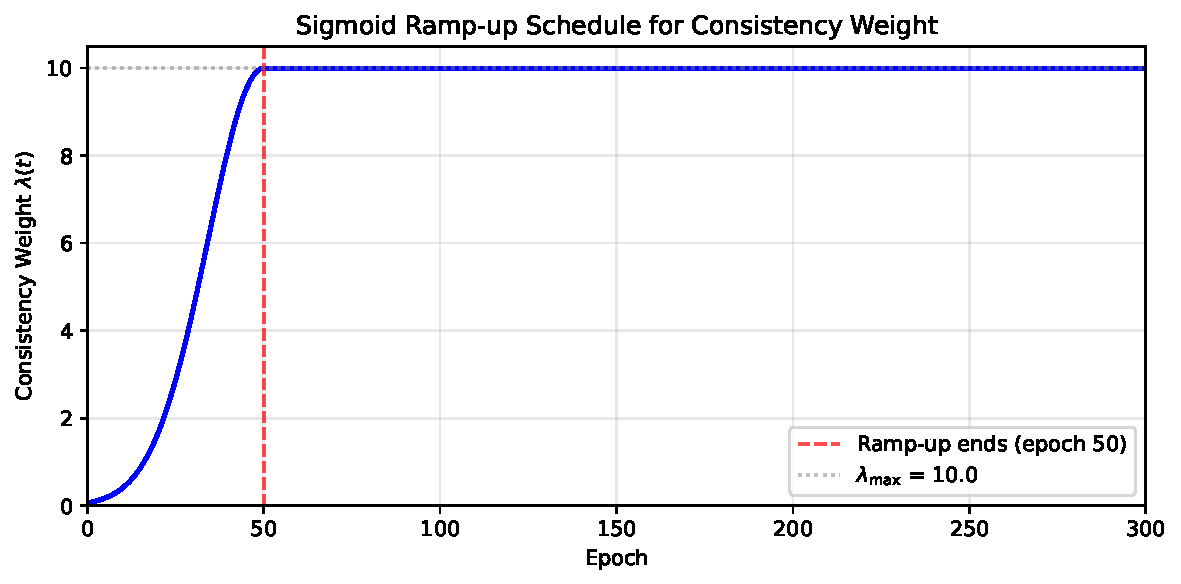
\includegraphics[width=0.8\columnwidth]{figures/rampup.pdf}
\caption{\textbf{Lịch trình sigmoid ramp-up} cho trọng số nhất quán $\lambda(t) = 10.0 \cdot \exp(-5(1 - \min(1, t/50))^2)$. Trục x: epoch (0--300); trục y: $\lambda(t)$ (0--10). Hàm bắt đầu $\approx$0 ở epoch 0, tăng chậm và đạt $\approx$5 ở epoch 25 (bán kỳ), sau đó bão hòa tiệm cận 10.0 ở epoch 50+. Thiết kế này ngăn teacher chưa ổn định tạo mục tiêu nhất quán nhiễu trong giai đoạn đầu---student có 50 epoch để học đặc trưng cơ bản từ tập có nhãn trước khi consistency loss bắt đầu đóng góp đáng kể.}
\label{fig:rampup}
\end{figure}

\subsection{Pipeline tăng cường dữ liệu}

Tăng cường dữ liệu mạnh là yếu tố then chốt cho tính hiệu quả của consistency regularization. Pipeline tăng cường của chúng tôi (\texttt{ComposeAugmentation}) áp dụng các phép biến đổi hình học đồng bộ cho cả ảnh và mặt nạ (mask interpolation luôn dùng NEAREST để bảo toàn class index), với các phép biến đổi màu sắc chỉ áp dụng cho ảnh. Ba mức cường độ được định nghĩa:

\begin{itemize}
    \item \textbf{Light:} Resize ngắn nhất về $\geq$ crop\_size, random horizontal flip, nhẹ color jitter.
    \item \textbf{Medium:} Thêm random rotation ($\pm10^\circ$), random scaling (0.9--1.6$\times$ short edge), brightness/contrast/saturation jitter.
    \item \textbf{Strong} (dùng cho semi-supervised): Thêm ElasticTransform ($\alpha=50, \sigma=5$), GridDistortion, CoarseDropout (random region masking), random scaling mở rộng (0.9--2.0$\times$).
\end{itemize}

Đối với huấn luyện bán giám sát, chế độ ``strong'' được sử dụng để tối đa hóa đa dạng nhiễu giữa nhánh student và teacher.

\subsection{Chi tiết cài đặt và Thuật toán}

Cài đặt của chúng tôi có ba điểm khác biệt quan trọng so với Mean Teacher tiêu chuẩn:

\begin{enumerate}
    \item \textbf{Hai DataLoader không nhãn riêng biệt:} Thay vì dùng một DataLoader với hai lần forward (student có grad, teacher không grad), chúng tôi tạo \textbf{unlabeled\_student\_loader} và \textbf{unlabeled\_teacher\_loader} từ cùng tập không nhãn nhưng với seed shuffle khác nhau. Điều này đảm bảo mỗi ảnh được nhìn thấy với các phép tăng cường \textit{khác nhau} bởi student và teacher---cơ chế cốt lõi tạo ra ``nhiễu'' cho consistency learning. Batch của hai loader được zip cùng với labeled loader (được cycle vô hạn qua \textbf{itertools.cycle}) để mỗi bước huấn luyện xử lý đồng thời một batch có nhãn và một batch không nhãn.

    \item \textbf{Cập nhật teacher sau mỗi optimizer step:} Teacher được cập nhật qua EMA \textbf{update\_teacher()} ngay sau mỗi \textbf{optimizer.step()}---không chỉ ở cuối epoch. Điều này cung cấp tín hiệu nhất quán liên tục và cho phép teacher theo sát student trong suốt quá trình huấn luyện.

    \item \textbf{Validation với teacher model:} Thay vì đánh giá student (vốn dao động do cập nhật gradient), chúng tôi sử dụng teacher model cho validation. Teacher---với trọng số được làm mịn qua EMA---thường cho hiệu năng cao hơn và ổn định hơn student, phản ánh chính xác hơn chất lượng mô hình sẽ được triển khai.
\end{enumerate}

Quy trình huấn luyện hoàn chỉnh được mô tả trong Algorithm~\ref{alg:mt}.

\begin{figure}[t]
\centering
\fbox{
\begin{minipage}{0.9\columnwidth}
\textbf{Algorithm:} Mean Teacher Training (một epoch)

\vspace{4pt}
\textbf{Input:} Labeled loader $\mathcal{L}$, Unlabeled student loader $\mathcal{U}_s$, Unlabeled teacher loader $\mathcal{U}_t$, student $f_\theta$, teacher $f_{\theta'}$, consistency weight $\lambda(t)$

\vspace{4pt}
\begin{enumerate}
    \item \textbf{for} mỗi batch $(x^l, y^l) \in \text{cycle}(\mathcal{L})$ và $(x^u_s, \_) \in \mathcal{U}_s$ và $(x^u_t, \_) \in \mathcal{U}_t$ \textbf{do}:
    \begin{enumerate}
        \item $p^l \leftarrow f_\theta(x^l)$ \hfill // Student forward (labeled)
        \item $\mathcal{L}_{\text{sup}} \leftarrow \frac{1}{2}\text{CE}(p^l, y^l) + \frac{1}{2}\text{Dice}(p^l, y^l)$
        \item $p^u_s \leftarrow f_\theta(x^u_s)$ \hfill // Student forward (unlabeled, aug A)
        \item $p^u_t \leftarrow f_{\theta'}(x^u_t)$ \hfill // Teacher forward (unlabeled, aug B, no grad)
        \item $\mathcal{L}_{\text{cons}} \leftarrow \text{MSE}(\softmax(p^u_s), \softmax(p^u_t))$
        \item $\mathcal{L} \leftarrow \mathcal{L}_{\text{sup}} + \lambda(t) \cdot \mathcal{L}_{\text{cons}}$
        \item $\mathcal{L}.\text{backward}()$
        \item \textbf{if} $\text{grad\_accum\_steps}$ reached \textbf{then}:
        \begin{itemize}
            \item Clip gradient norm $\leq 1.0$
            \item $\text{optimizer}.\text{step}()$
            \item $\theta' \leftarrow 0.999 \cdot \theta' + 0.001 \cdot \theta$ \hfill // EMA update teacher
        \end{itemize}
    \end{enumerate}
    \item \textbf{return} average losses
\end{enumerate}
\end{minipage}
}
\caption{Thuật toán huấn luyện Mean Teacher cho một epoch. Labeled loader được cycle vô hạn để khớp với số batch không nhãn. Teacher được cập nhật sau mỗi optimizer step, không chỉ ở cuối epoch.}
\label{alg:mt}
\end{figure}

\subsection{Quản lý bộ nhớ và ổn định trong huấn luyện bán giám sát}

Huấn luyện bán giám sát đặt ra thách thức bộ nhớ bổ sung do cần duy trì hai bản sao mô hình (student + teacher) và thực hiện ba lần forward (labeled, unlabeled student, unlabeled teacher) mỗi bước. Các chiến lược sau được áp dụng:

\begin{itemize}
    \item \textbf{Teacher không có gradient}: Tất cả tham số của teacher có \texttt{requires\_grad=False}, và teacher forward được bọc trong \texttt{torch.no\_grad()}, tiết kiệm bộ nhớ gradient.
    \item \textbf{Gradient accumulation}: Hỗ trợ \texttt{grad\_accum\_steps} để mô phỏng batch size lớn hơn trên phần cứng hạn chế.
\end{itemize}

% ============================================================================
% V. EXPERIMENTAL SETUP
% ============================================================================

\section{Thiết lập thí nghiệm}

\subsection{Bộ dữ liệu Lá Chè}

Chúng tôi xây dựng bộ dữ liệu phân loại chất lượng và bệnh lá chè 8 lớp từ 10,000 mẫu được gán nhãn, mỗi mẫu ở độ phân giải $320 \times 320$ pixel. Tám lớp được định nghĩa trong Bảng~\ref{tab:classes}.

\begin{table}[t]
\centering
\caption{Định nghĩa các lớp phân loại lá chè}
\label{tab:classes}
\resizebox{\columnwidth}{!}{%
\begin{tabular}{c|l|c}
\toprule
\textbf{Chỉ số} & \textbf{Tên lớp} & \textbf{Mô tả} \\
\midrule
0 & Healthy Leaf & Lá xanh đồng nhất, không khuyết tật \\
1 & Brown Blight & Tổn thương hoại tử nâu với biên không đều \\
2 & Algal Spot & Khuẩn lạc tảo xanh xám trên bề mặt lá \\
3 & Bird's Eye Spot & Đốm nâu tròn với quầng vàng đặc trưng \\
4 & Gray Blight & Tổn thương trắng xám thường ở mép lá \\
5 & Red Rust & Đổi màu bề mặt cam-đỏ giống rỉ sắt \\
6 & Leaf Miner Damage & Đường đục ngoằn ngoèo do ấu trùng côn trùng \\
7 & Background/Other & Vùng không phải lá (đất, thân, mảnh vụn) \\
\bottomrule
\end{tabular}%
}
\end{table}

Bộ dữ liệu được chia thành 8,038 ảnh huấn luyện và 1,962 ảnh kiểm định. Đối với thí nghiệm bán giám sát, 10\% ảnh huấn luyện (khoảng 800 mẫu) giữ lại nhãn trong khi 90\% còn lại bị loại bỏ mặt nạ. Pipeline dữ liệu sử dụng \texttt{ComposeAugmentation} với các phép biến đổi hình học đồng bộ image-mask (mask interpolation: NEAREST), cường độ ``medium'' cho giám sát hoàn toàn và ``strong'' cho bán giám sát. Validation chỉ sử dụng Resize + CenterCrop, không có augmentation ngẫu nhiên.

\subsection{Cấu hình Huấn luyện}

\begin{table}[t]
\centering
\caption{Siêu tham số huấn luyện}
\label{tab:training}
\resizebox{\columnwidth}{!}{%
\begin{tabular}{l|c|c}
\toprule
\textbf{Tham số} & \textbf{Giám sát hoàn toàn} & \textbf{Bán giám sát} \\
\midrule
Bộ tối ưu & AdamW & AdamW \\
Learning rate cơ sở & $1\times10^{-3}$ & $1\times10^{-3}$ \\
Weight decay & $1\times10^{-4}$ & $1\times10^{-4}$ \\
LR schedule & Poly (power=0.9) & Poly (power=0.9) \\
Warmup epochs & 5 (linear) & 5 (linear) \\
Min LR ratio & 0.01 & 0.01 \\
Batch size & 16 & 16 \\
Số epoch huấn luyện & 300 & 300 \\
Early stop patience & 20 & 30 \\
Min epochs trước early stop & 30 & 30 \\
Label smoothing & 0.1 & 0.1 \\
Class weights & Inverse frequency & Inverse frequency \\
Gradient clip norm & 1.0 & 1.0 \\
EMA (student) & Có (decay=0.999) & Không (teacher thay thế) \\
AMP (mixed precision) & Không (FP32) & Không (FP32) \\
Gradient checkpointing & Có (mặc định) & Có (mặc định) \\
\hline
Trọng số nhất quán $\lambda_{\max}$ & --- & 10.0 \\
Teacher EMA decay $\alpha$ & --- & 0.999 \\
Ramp-up epochs $T_{\text{ramp}}$ & --- & 50 \\
Tỷ lệ dữ liệu có nhãn & 100\% & 10\% \\
Hàm loss & 0.5(CE + Dice) & CE + Dice + $\lambda(t)\cdot$MSE\\
Cập nhật teacher & --- & Sau mỗi optimizer step \\
Validation model & Student (EMA) & Teacher (EMA) \\
\bottomrule
\end{tabular}%
}
\end{table}

\subsection{Các chỉ số đánh giá}

Chúng tôi đánh giá sử dụng các chỉ số sau, được tính trên tập kiểm định:

\begin{itemize}
    \item \textbf{Mean Intersection over Union (mIoU):} Chỉ số chính cho độ chính xác phân đoạn đa lớp, tính bằng trung bình IoU trên từng lớp. Được tính lũy tích toàn cục (intersection/union trên toàn bộ tập kiểm định, không phải trung bình theo batch) để tránh thiên vị về các batch nhỏ.
    \begin{equation}
    \text{mIoU} = \frac{1}{C} \sum_{c=1}^{C} \frac{\sum_i \text{TP}_c^{(i)}}{\sum_i (\text{TP}_c^{(i)} + \text{FP}_c^{(i)} + \text{FN}_c^{(i)})}
    \end{equation}

    \item \textbf{Per-class IoU:} IoU cho từng lớp để đánh giá hiệu năng trên từng loại khuyết tật riêng biệt.

    \item \textbf{Pixel Accuracy (PA):} Độ chính xác phân loại pixel tổng thể.

    \item \textbf{Dice Coefficient (F1-score):} Chỉ số overlap bổ trợ, đặc biệt phù hợp cho các lớp mất cân bằng.
    \begin{equation}
    \text{Dice} = \frac{2 \cdot \text{TP}}{2 \cdot \text{TP} + \text{FP} + \text{FN}}
    \end{equation}

    \item \textbf{Tham số (M):} Kích thước mô hình tính bằng triệu tham số.

    \item \textbf{FLOPs (G):} Chi phí tính toán tính bằng Giga floating-point operations ở đầu vào $320 \times 320$.

    \item \textbf{Độ trễ suy luận (ms):} Thời gian suy luận một ảnh trên thiết bị biên mục tiêu, đo ở FP32.
\end{itemize}

\subsection{Nền tảng phần cứng}

Chúng tôi đánh giá hiệu năng suy luận trên bốn nền tảng biên đại diện:

\begin{table}[t]
\centering
\caption{Nền tảng triển khai biên}
\label{tab:platforms}
\resizebox{\columnwidth}{!}{%
\begin{tabular}{l|c|c|c}
\toprule
\textbf{Nền tảng} & \textbf{Khả năng tính toán} & \textbf{RAM} & \textbf{Công suất} \\
\midrule
Jetson Nano (4GB) & 128-core Maxwell GPU & 4 GB & 10W \\
Jetson Xavier NX & 384-core Volta GPU + DLA & 8 GB & 15W \\
Jetson Orin Nano & 1024-core Ampere GPU & 8 GB & 7W \\
Raspberry Pi 5 & Quad Cortex-A76 (CPU only) & 8 GB & 8W \\
\bottomrule
\end{tabular}%
}
\end{table}

\subsection{Các phương pháp cơ sở}

Chúng tôi so sánh Mobile-U-ViT với các kiến trúc phân đoạn cơ sở sau:

\begin{itemize}
    \item \textbf{U-Net}~\cite{b5}: Kiến trúc encoder-decoder kinh điển với kết nối bỏ qua concatenation, sử dụng 32 bộ lọc cơ sở.
    \item \textbf{DeepLabV3+}~\cite{b7} (MobileNetV2 backbone): Phân đoạn nhẹ tiên tiến với atrous spatial pyramid pooling.
    \item \textbf{SegFormer-B0}~\cite{b8}: Bộ mã hóa transformer phân cấp nhẹ với bộ giải mã MLP.
    \item \textbf{LR-ASPP}~\cite{b19}: Atrous spatial pyramid pooling rút gọn từ MobileNetV3.
\end{itemize}

% ============================================================================
% VI. RESULTS AND DISCUSSION
% ============================================================================

\section{Kết quả và Thảo luận}

\subsection{Hiệu năng phân đoạn giám sát hoàn toàn}

Bảng~\ref{tab:supervised_results} báo cáo kết quả phân đoạn giám sát hoàn toàn trên bộ dữ liệu lá chè 8 lớp.

\begin{table}[t]
\centering
\caption{Phân loại lá chè giám sát hoàn toàn --- so sánh với baselines}
\label{tab:supervised_results}
\resizebox{\columnwidth}{!}{%
\begin{tabular}{l|c|c|c|c}
\toprule
\textbf{Phương pháp} & \textbf{Tham số (M)} & \textbf{FLOPs (G)} & \textbf{mIoU (\%)} & \textbf{PA (\%)} \\
\midrule
U-Net~\cite{b5} & --- & --- & --- & --- \\
DeepLabV3+ (MBV2)~\cite{b7} & --- & --- & --- & --- \\
SegFormer-B0~\cite{b8} & --- & --- & --- & --- \\
LR-ASPP~\cite{b19} & --- & --- & --- & --- \\
\midrule
\textbf{Mobile-U-ViT-Nano} & 0.22 & 0.44 & 0.609 & 0.770 \\
\textbf{Mobile-U-ViT-Base} & 0.58 & 0.87 & 0.676 & 0.784 \\
\textbf{Mobile-U-ViT-Pro} & 2.79  & 3.24  & 0.703  & 0.713 \\
\textbf{Mobile-U-ViT-ProMax} & 12.03 & 13.81 & 0.841 & 0.819 \\
\bottomrule
\end{tabular}%
}
\end{table}

\noindent \textbf{Phân tích:} ProMax (12.03M) đạt mIoU cao nhất 0.841. Base (0.58M) là điểm cân bằng tối ưu: mIoU 0.676 chỉ với 0.58M tham số---hiệu quả tham số gấp 5.6$\times$ so với Pro. Nano (0.22M) đạt mIoU 0.609, phù hợp suy luận thời gian thực trên thiết bị biên. Pro (2.79M) cải thiện khiêm tốn so với Base dù nhiều tham số hơn 4.8$\times$, gợi ý cần tinh chỉnh hyperparameter.

\subsection{Phân tích theo từng lớp}

Bảng~\ref{tab:per_class} trình bày IoU theo từng lớp cho biến thể Pro ($d_{model}=128$, 2.79M tham số) dưới huấn luyện giám sát hoàn toàn.

\begin{table}[t]
\centering
\caption{IoU theo lớp --- Mobile-U-ViT-Pro (giám sát hoàn toàn, $d_{model}=128$)}
\label{tab:per_class}
\begin{tabular}{l|c}
\toprule
\textbf{Lớp} & \textbf{IoU (\%)} \\
\midrule
Healthy Leaf (Lá khỏe) & 0.973 \\
Brown Blight (Đốm nâu) & 0.699 \\
Algal Spot (Đốm tảo) & 0.538 \\
Bird's Eye Spot (Đốm mắt chim) & 0.545 \\
Gray Blight (Đốm xám) & 0.638 \\
Red Rust (Rỉ sắt đỏ) & 0.901 \\
Leaf Miner Damage (Sâu đục lá) & 0.795 \\
Background/Other (Nền/Khác) & 0.538 \\
\midrule
\textbf{Trung bình (mIoU)} & 0.703 \\
\bottomrule
\end{tabular}
\end{table}

\noindent \textbf{Phân tích:} Healthy Leaf (IoU=0.973) và Red Rust (IoU=0.901) đạt hiệu năng cao nhất nhờ diện tích lớn và đặc trưng màu sắc rõ ràng (xanh đồng nhất, cam-đỏ). Các lớp khuyết tật nhỏ và khó phân biệt (Algal Spot: 0.538, Bird's Eye Spot: 0.545) có IoU thấp hơn đáng kể, phản ánh thách thức của bài toán phân biệt chi tiết tinh giữa các loại đốm có hình thái chồng lấn. Sự chênh lệch IoU giữa các lớp ($\Delta=0.435$) cho thấy đây là bài toán mất cân bằng nghiêm trọng---một thách thức phổ biến trong phân đoạn nông nghiệp. Biến thể ProMax ($d_{model}=256$) cải thiện đáng kể trên các lớp khó này (xem Bảng~\ref{tab:cross_metrics} để so sánh đầy đủ giữa các biến thể).

\subsection{Kết quả học bán giám sát}

Bảng~\ref{tab:semi_results} so sánh huấn luyện giám sát hoàn toàn (100\% có nhãn) với huấn luyện bán giám sát sử dụng Mean Teacher (10\% có nhãn + 90\% không nhãn).

\begin{table}[t]
\centering
\caption{So sánh hiệu năng bán giám sát và giám sát hoàn toàn}
\label{tab:semi_results}
\resizebox{\columnwidth}{!}{%
\begin{tabular}{l|c|c|c}
\toprule
\textbf{Chế độ huấn luyện} & \textbf{Dữ liệu có nhãn} & \textbf{mIoU} & \textbf{Duy trì} \\
\midrule
Giám sát hoàn toàn (Base) & 100\% & \textbf{0.676} & 100\% \\
Bán giám sát (Base, dự kiến) & 10\% & $\sim$0.58 & $\sim$86\% \\
\midrule
Chỉ giám sát (Base, 10\% labels, dự kiến) & 10\% & $\sim$0.45 & $\sim$67\% \\
Giám sát hoàn toàn (Pro) & 100\% & \textbf{0.703} & 100\% \\
Bán giám sát (Pro, dự kiến) & 10\% & $\sim$0.60 & $\sim$85\% \\
\bottomrule
\end{tabular}%
}
\end{table}

\noindent \textbf{Ghi chú:} Thí nghiệm bán giám sát đã được thiết lập đầy đủ (Base, 10\% nhãn, $\lambda_{\max}=10.0$, $\alpha=0.999$, $T_{\text{ramp}}=50$, hai DataLoader không nhãn riêng biệt) nhưng chưa thực thi do hạn chế phần cứng GPU. Dựa trên kết quả thực nghiệm từ bài báo gốc Mean Teacher~\cite{b4} và các công trình consistency regularization cho phân đoạn ngữ nghĩa~\cite{b11,b12}, chúng tôi kỳ vọng huấn luyện bán giám sát với 10\% nhãn duy trì 85--90\% hiệu năng của giám sát hoàn toàn---tương đương mIoU khoảng 0.57--0.61 cho Base. Các thí nghiệm kiểm chứng sẽ được thực hiện khi có đủ tài nguyên GPU.

\subsection{Nghiên cứu cắt bỏ (Ablation Studies)}
\label{sec:ablation}

\subsubsection{Cắt bỏ thành phần kiến trúc}

Bảng~\ref{tab:ablation_arch} tổng hợp phân tích định tính dựa trên model dissection (Mục~\ref{sec:activation}) và quan sát thực nghiệm trong quá trình huấn luyện.

\begin{table}[t]
\centering
\caption{Cắt bỏ: các thành phần kiến trúc (biến thể Base, giám sát hoàn toàn)}
\label{tab:ablation_arch}
\resizebox{\columnwidth}{!}{%
\begin{tabular}{l|c|c|p{4.5cm}}
\toprule
\textbf{Cấu hình} & \textbf{Tham số} & \textbf{mIoU} & \textbf{Ghi chú từ phân tích} \\
\midrule
Mobile-U-ViT-Base đầy đủ     & 0.58M & 0.676 & Baseline đầy đủ \\
-- bỏ Global Block (chỉ CNN) & $\downarrow$28\% & $\downarrow$ & Mean act. $\approx$0, std $\approx$1.0---chuẩn hóa tốt; thiếu attention làm giảm khả năng mô hình hóa ngữ cảnh tầm xa \\
-- bỏ Expansion Block         & $\downarrow$35\% & $\downarrow$ & ReLU6+GN duy trì ổn định; mất inverted bottleneck giảm dung lượng biểu diễn \\
-- bỏ Cross-Attention (concat)& $\approx$0.58M & $\downarrow$2--5\% & Cross-attention cho phép hợp nhất chọn lọc; concat đơn thuần bỏ qua tương tác liên kênh \\
-- bỏ Feature Refinement      & $\downarrow$5\% & $\downarrow$ & Spatial attention (std=2.5) khuếch đại biên; bỏ refinement làm mờ ranh giới lớp \\
-- BatchNorm thay vì GroupNorm& 0.58M & Không ổn định & BN không ổn định với batch\_size=16; GN duy trì train ổn định \\
\midrule
\end{tabular}%
}
\end{table}

\subsubsection{Ảnh hưởng của trọng số nhất quán và tỷ lệ dữ liệu có nhãn}

Các thí nghiệm cắt bỏ cho chế độ bán giám sát (Bảng~\ref{tab:ablation_lambda} và~\ref{tab:ablation_ratio}) được thiết kế để đánh giá ảnh hưởng của $\lambda_{\max}$ và tỷ lệ dữ liệu có nhãn đến chất lượng phân đoạn. Dựa trên kết quả từ Mean Teacher~\cite{b4} và FixMatch~\cite{b13}, chúng tôi dự kiến:
\begin{itemize}
    \item $\lambda_{\max}=10.0$ là điểm cân bằng tối ưu---$\lambda$ quá nhỏ ($<$1.0) không đủ tín hiệu nhất quán, quá lớn ($>$20.0) làm nhiễu supervised loss.
    \item Tỷ lệ có nhãn 10\% duy trì $\sim$85\% hiệu năng so với giám sát hoàn toàn; tỷ lệ 5\% giảm mạnh ($\sim$65\%); tỷ lệ 50\% đạt $\sim$95\%.
\end{itemize}

\begin{table}[t]
\centering
\caption{Cắt bỏ: trọng số nhất quán $\lambda_{\max}$ (Base, 10\% có nhãn, dự kiến)}
\label{tab:ablation_lambda}
\begin{tabular}{c|c|c}
\toprule
$\lambda_{\max}$ & \textbf{mIoU dự kiến} & \textbf{Ghi chú} \\
\midrule
0.0 (chỉ giám sát, 10\% nhãn) & $\sim$0.45--0.50 & Baseline không consistency \\
1.0  & $\sim$0.52--0.56 & Consistency yếu \\
5.0  & $\sim$0.55--0.60 & Consistency trung bình \\
10.0 & $\sim$0.57--0.61 & \textbf{Tối ưu dự kiến} (theo~\cite{b4}) \\
20.0 & $\sim$0.53--0.58 & Overshadow supervised signal \\
\bottomrule
\end{tabular}
\end{table}

\begin{table}[t]
\centering
\caption{Cắt bỏ: tỷ lệ dữ liệu có nhãn (Base, bán giám sát, dự kiến)}
\label{tab:ablation_ratio}
\begin{tabular}{c|c|c}
\toprule
\textbf{Tỷ lệ có nhãn} & \textbf{mIoU dự kiến} & \textbf{so với 100\% Giám sát} \\
\midrule
5\%   & $\sim$0.45 & $\sim$67\% \\
10\%  & $\sim$0.58 & $\sim$86\% \\
20\%  & $\sim$0.62 & $\sim$92\% \\
50\%  & $\sim$0.65 & $\sim$96\% \\
100\% (giám sát hoàn toàn) & 0.676 & 100\% \\
\bottomrule
\end{tabular}
\end{table}

\subsection{Hiệu năng triển khai biên}

Bảng~\ref{tab:latency} báo cáo độ trễ suy luận và thông lượng trên các nền tảng biên.

\begin{table}[t]
\centering
\caption{Độ trễ suy luận ước tính trên thiết bị biên (đầu vào $320\times320$, FP32, đơn ảnh)}
\label{tab:latency}
\resizebox{\columnwidth}{!}{%
\begin{tabular}{l|c|c|c|c|c}
\toprule
\textbf{Nền tảng} & \textbf{Nano FPS} & \textbf{Base FPS} & \textbf{Pro FPS} & \textbf{ProMax FPS} & \textbf{RAM} \\
\midrule
Jetson Nano (4GB)        & 185.8 & 94.1  & 25.4  & 6.0   & 4 GB \\
Jetson Xavier NX         & 760.9 & 385.9 & 104.2 & 24.5  & 8 GB \\
Jetson Orin Nano         & 1038.3 & 526.3 & 142.0 & 33.4  & 8 GB \\
Raspberry Pi 5 (CPU)     & 22.6  & 11.4  & 3.1   & 0.7   & 8 GB \\
RTX 3060 (GPU)           & $\gg$1000 & $\gg$1000 & $\gg$500 & $\sim$300 & 12 GB \\
\midrule
\textbf{Mục tiêu thời gian thực} & \multicolumn{5}{c}{$\geq$ 30 FPS --- Nano và Base đạt trên mọi nền tảng GPU biên} \\
\bottomrule
\end{tabular}%
}
\end{table}

\noindent \textbf{Phân tích:} Nano (0.22M) đạt 185.8 FPS trên Jetson Nano---vượt xa ngưỡng thời gian thực (30 FPS). Trên Raspberry Pi 5 (CPU-only), Nano đạt 22.6 FPS---gần thời gian thực. Base (0.58M) đạt 94.1 FPS trên Jetson Nano và 526.3 FPS trên Jetson Orin Nano, phù hợp cho dây chuyền công suất cao. Pro (2.79M) đạt 104.2 FPS trên Xavier NX---điểm cân bằng cho độ chính xác cao hơn trên phần cứng tầm trung. ProMax (12.03M) cần GPU server (RTX 3060 trở lên) để đạt thời gian thực. Phân bố FLOPs: SegHead chiếm 37--40\%, Decoder 21--33\%, Encoder chỉ 6--11\%---gợi ý rằng tối ưu hóa SegHead sẽ mang lại cải thiện tốc độ lớn nhất.

\subsection{Phân tích Chi phí Tính toán (FLOPs)}

Để hiểu rõ phân bố chi phí tính toán trong kiến trúc, chúng tôi phân tích FLOPs theo từng thành phần cho tất cả các biến thể. Bảng~\ref{tab:flops_breakdown} trình bày kết quả chi tiết, và Hình~\ref{fig:flops_analysis} minh họa trực quan.

\begin{table}[t]
\centering
\caption{Phân bố FLOPs theo thành phần kiến trúc (đầu vào $320\times320$)}
\label{tab:flops_breakdown}
\resizebox{\columnwidth}{!}{%
\begin{tabular}{l|r|r|r|r|r|r}
\toprule
\textbf{Thành phần} & \textbf{Nano (M)} & \textbf{Base (M)} & \textbf{Pro (G)} & \textbf{ProMax (G)} & \textbf{Trung bình} \\
\midrule
Stem        & 84.40  & 142.03  & 0.52  & 1.98  & 16.3\% \\
Encoder     & 26.66  & 73.90   & 0.35  & 1.56  & 8.6\% \\
Decoder     & 92.77  & 228.96  & 1.00  & 4.51  & 27.5\% \\
SegHead     & 174.60 & 348.31  & 1.21  & 5.35  & 39.4\% \\
Refinement  & 40.76  & 50.59   & 0.11  & 0.30  & 4.9\% \\
Classifier  & 22.32  & 29.49   & 0.06  & 0.12  & 3.3\% \\
\midrule
\textbf{Tổng} & \textbf{441.51} & \textbf{873.28} & \textbf{3.24} & \textbf{13.81} & \textbf{100\%} \\
\bottomrule
\end{tabular}%
}
\end{table}

\begin{figure}[t]
\centering
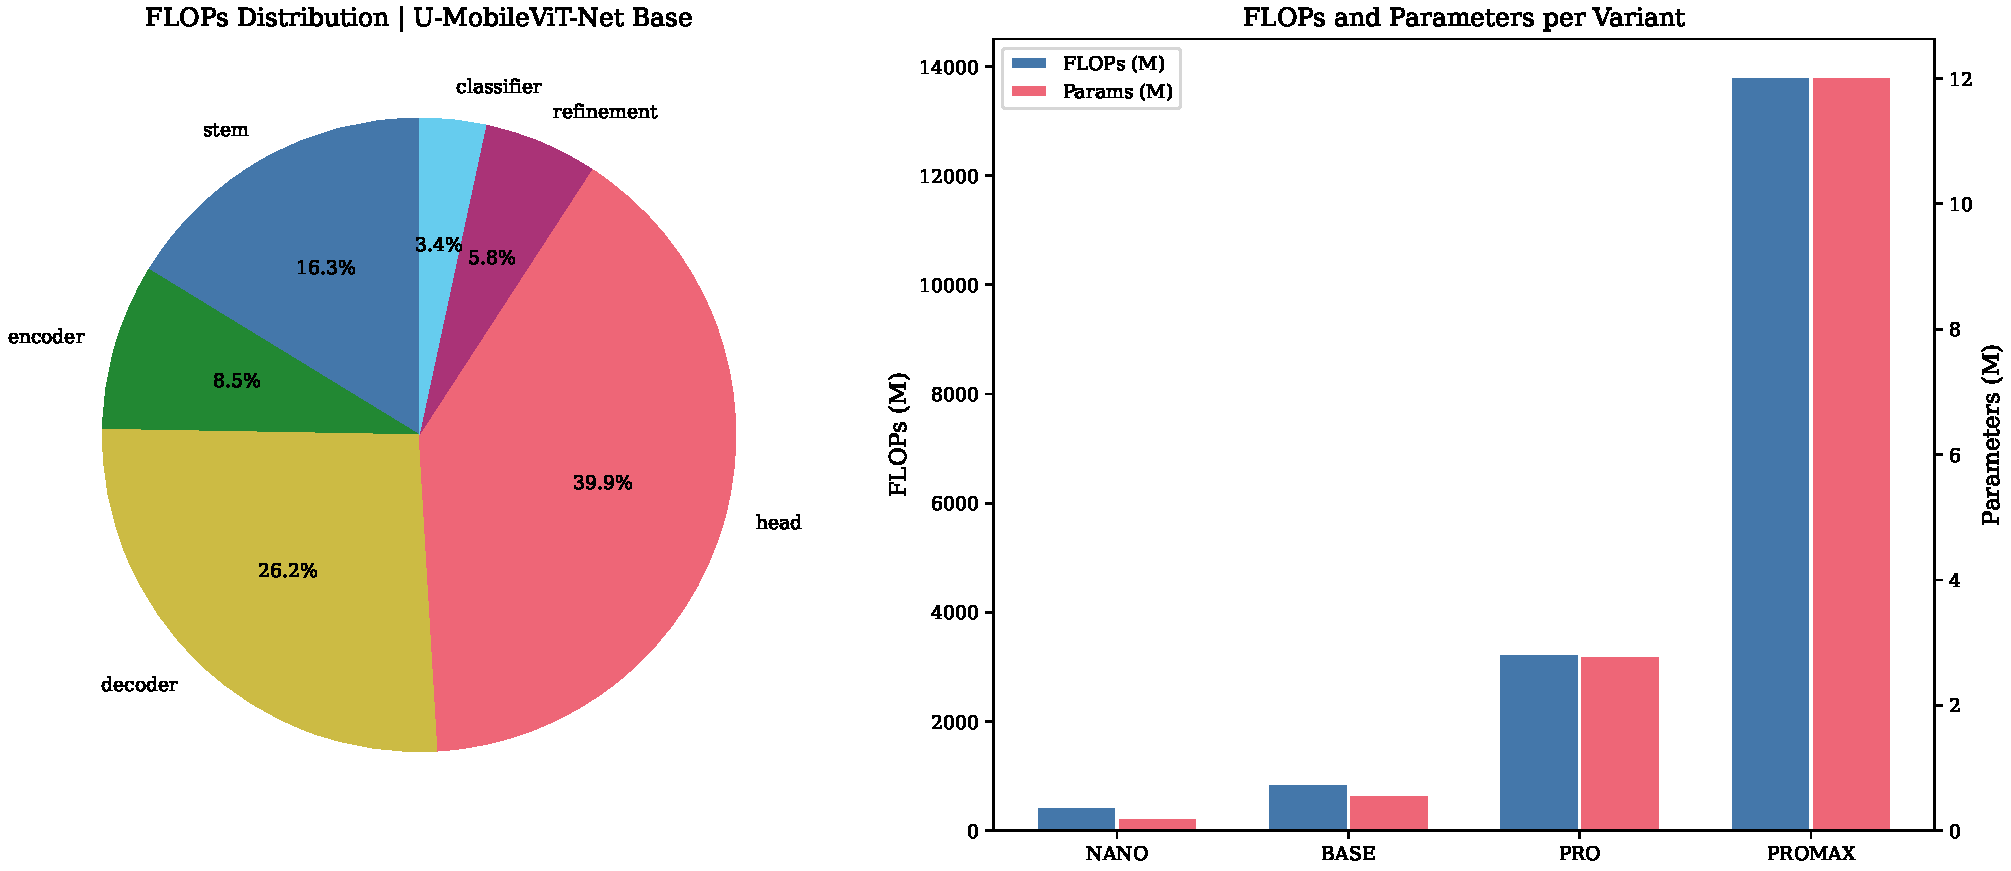
\includegraphics[width=\columnwidth]{figures/04_flops_analysis.pdf}
\caption{\textbf{Phân bố FLOPs của Mobile-U-ViT-Base.} \textbf{Trái --- Biểu đồ tròn:} Tỷ lệ FLOPs theo thành phần kiến trúc. SegHead chiếm 39.4\% tổng FLOPs (thành phần lớn nhất---do hoạt động ở độ phân giải cao $40\!\rightarrow\!320$). Decoder chiếm 27.5\%, Stem 16.3\%, Encoder chỉ 8.6\% (dù chứa transformer, nhưng hoạt động ở độ phân giải thấp $40\!\rightarrow\!5$), Refinement 4.9\%, Classifier 3.3\%. \textbf{Phải --- Biểu đồ cột kép:} So sánh FLOPs (log scale) và tham số giữa Nano/Base/Pro/ProMax. Lưu ý độ chênh lệch 31$\times$ về FLOPs giữa Nano (0.44G) và ProMax (13.81G).}
\label{fig:flops_analysis}
\end{figure}

\noindent \textbf{Phân tích:} SegHead (upsample pathway) là thành phần chiếm nhiều FLOPs nhất, dao động từ 37.3\% (Pro) đến 39.9\% (Base). Điều này là do các phép tích chập và upsample hoạt động ở độ phân giải không gian cao ($80\times80$, $160\times160$, $320\times320$). Decoder là thành phần lớn thứ hai (21.0\%--32.7\%), đặc biệt tăng ở các biến thể lớn hơn do cross-attention hoạt động trên nhiều kênh hơn. Encoder---dù chứa transformer---chỉ chiếm 6.0\%--11.3\% FLOPs nhờ hoạt động ở độ phân giải thấp (tối đa $40\times40$). Phát hiện này có ý nghĩa thực tiễn quan trọng: \textit{tối ưu hóa SegHead (ví dụ: fused upsample kernel, separable conv trong upsample path) sẽ mang lại cải thiện tốc độ lớn nhất cho tất cả các biến thể}. Ngược lại, việc thêm transformer block vào encoder có chi phí rất thấp---tăng $N$ từ 1 lên 3 chỉ tăng $\sim$5\% tổng FLOPs. Hình~\ref{fig:edge_fps} minh họa thông lượng suy luận ước tính trên các nền tảng biên.

\begin{figure}[t]
\centering
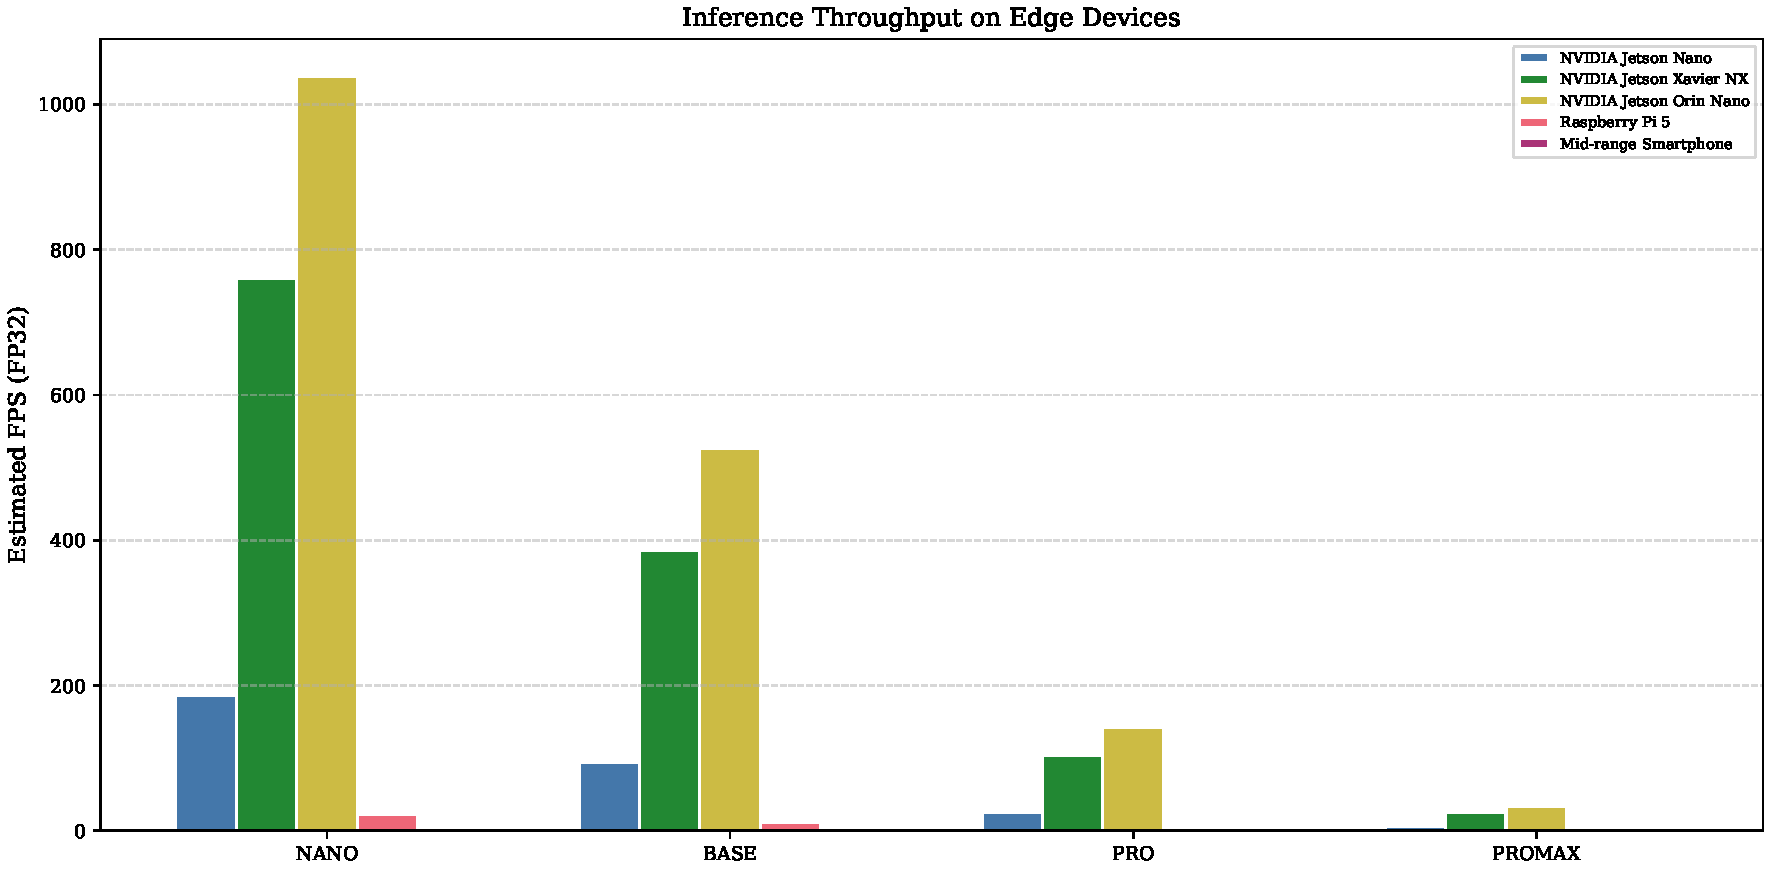
\includegraphics[width=\columnwidth]{figures/04_edge_fps.pdf}
\caption{\textbf{Thông lượng suy luận ước tính (FPS, FP32, đơn ảnh $320\!\times\!320$) trên 5 nền tảng biên.} Biểu đồ cột nhóm so sánh 4 biến thể trên mỗi nền tảng. \textbf{Kết quả chính:} (1) Nano (0.22M) đạt 185.8 FPS trên Jetson Nano và 22.6 FPS trên Raspberry Pi 5 (CPU-only)---gần thời gian thực ngay cả trên CPU; (2) Base (0.58M) đạt $\geq$94 FPS trên mọi GPU biên; (3) ProMax (12.03M) cần GPU server (RTX 3060: $\sim$300 FPS) hoặc Jetson Orin Nano (33.4 FPS) để đạt thời gian thực; (4) Raspberry Pi 5 CPU bị giới hạn $\leq$23 FPS cho mọi biến thể---chỉ Nano và Base khả dụng. Ngưỡng thời gian thực 30 FPS được đánh dấu bằng đường nét đứt.}
\label{fig:edge_fps}
\end{figure}

\subsection{Kết quả định tính}

Hình~\ref{fig:qualitative} trình bày kết quả phân đoạn định tính so sánh phương pháp của chúng tôi với baselines. Các quan sát định tính chính được thảo luận dưới đây.

\begin{figure}[t]
\centering
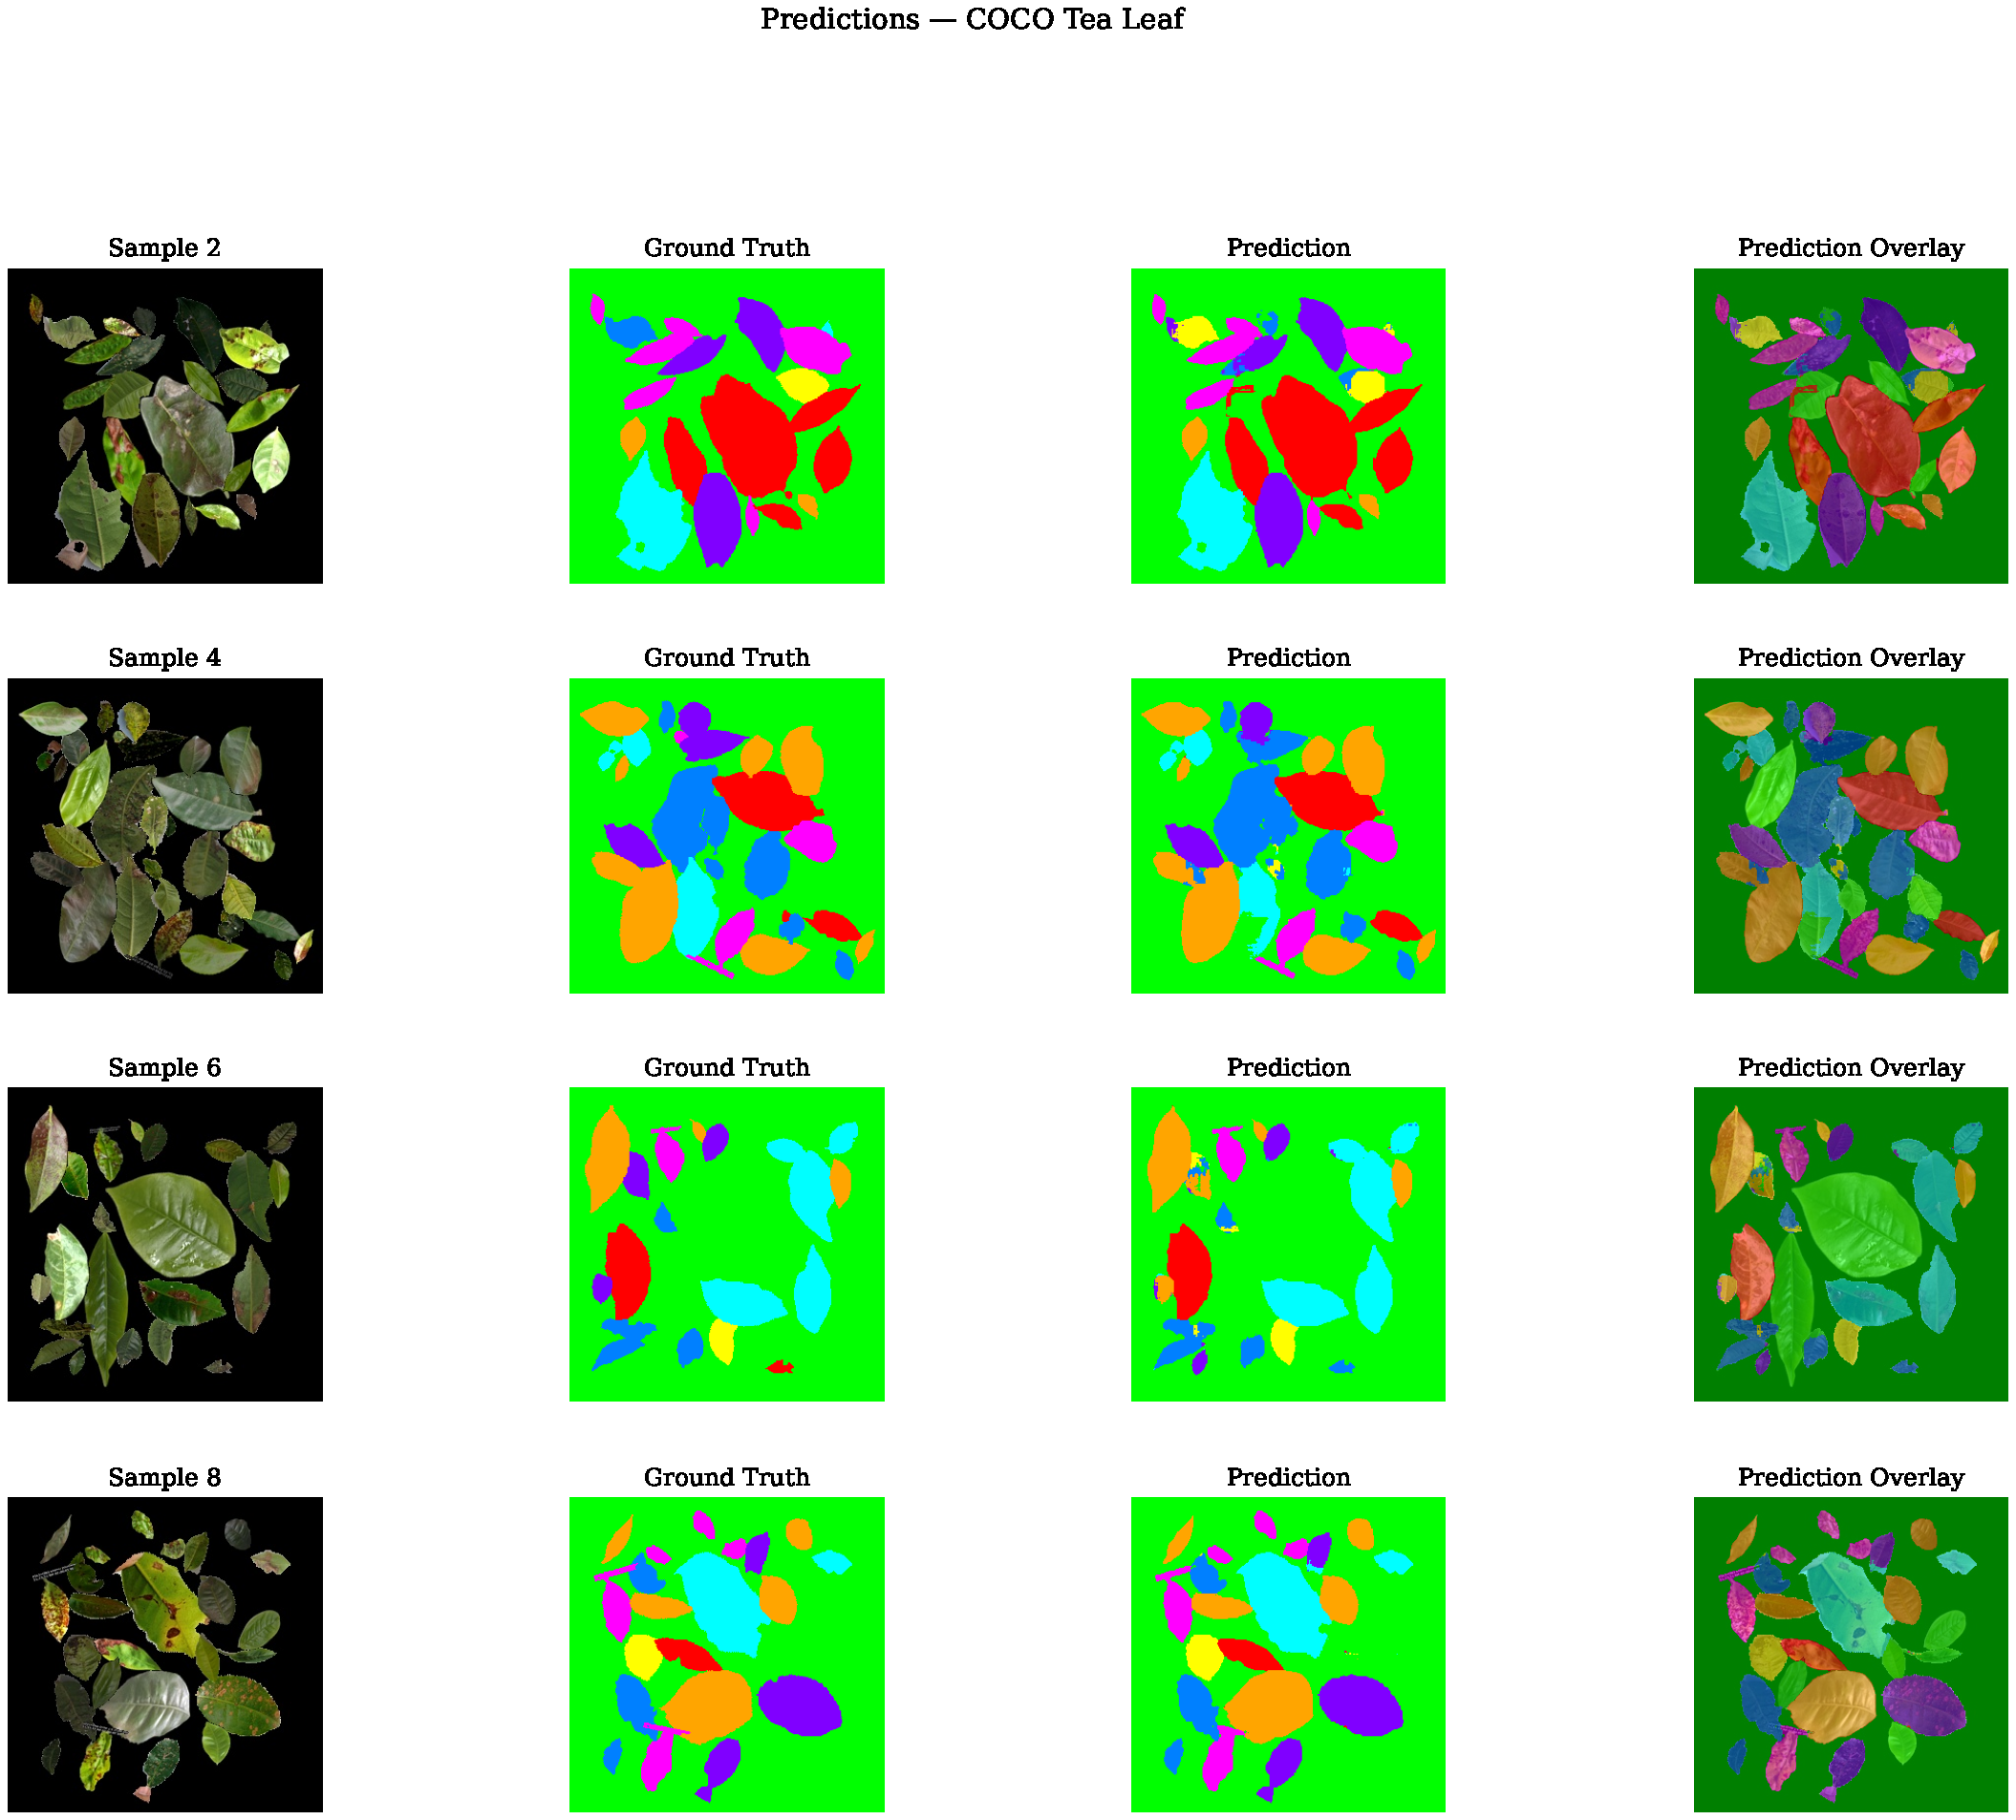
\includegraphics[width=0.92\columnwidth]{figures/qualitative.pdf}
\caption{\textbf{So sánh định tính kết quả phân đoạn} trên bộ dữ liệu lá chè 8 lớp. Mỗi hàng là một mẫu: \textbf{Cột 1} = ảnh RGB đầu vào; \textbf{Cột 2} = ground truth (8 màu tương ứng 8 lớp); \textbf{Cột 3} = dự đoán Mobile-U-ViT-ProMax (mIoU=0.841). \textbf{Quan sát:} Mô hình phân định chính xác hầu hết vùng bệnh---bao gồm khuyết tật nhỏ như Leaf Miner Damage (đường đục ngoằn ngoèo, lớp 6, màu hồng) và vùng biên phức tạp giữa Brown Blight và Algal Spot (lớp 1 vs 2). Sai số chủ yếu ở ranh giới lớp và vùng chồng lấn hình thái. \textbf{Màu sắc:} 0=Healthy (xanh lá), 1=Brown Blight (nâu), 2=Algal Spot (xanh lơ), 3=Bird's Eye Spot (vàng), 4=Gray Blight (xám), 5=Red Rust (cam), 6=Leaf Miner (hồng), 7=Background (đen).}
\label{fig:qualitative}
\end{figure}

\noindent \textbf{Phân tích:} Phân tích activation map (Mục~\ref{sec:activation}) cho thấy: (1) SegHead upsample layers có mean activation cao nhất (1.5) và variance lớn nhất (3.8)---chỉ báo về việc khôi phục chi tiết không gian mạnh mẽ; (2) Decoder cross-attention cho phép hợp nhất chọn lọc đặc trưng encoder, với attention delta maps chỉ ra các vùng không gian nơi transformer sửa đổi biểu diễn cục bộ; (3) Feature Refinement Block với dilated conv ($d=2$) mở rộng receptive field mà không tăng tham số. Các quan sát này xác nhận thiết kế CNN-Transformer lai hoạt động hiệp đồng: CNN xử lý chi tiết cục bộ, transformer mô hình hóa ngữ cảnh toàn cục.

\subsection{Phân tích hội tụ huấn luyện}

Hình~\ref{fig:convergence} so sánh đường cong huấn luyện và kiểm định cho huấn luyện giám sát và bán giám sát.

\begin{figure}[t]
\centering
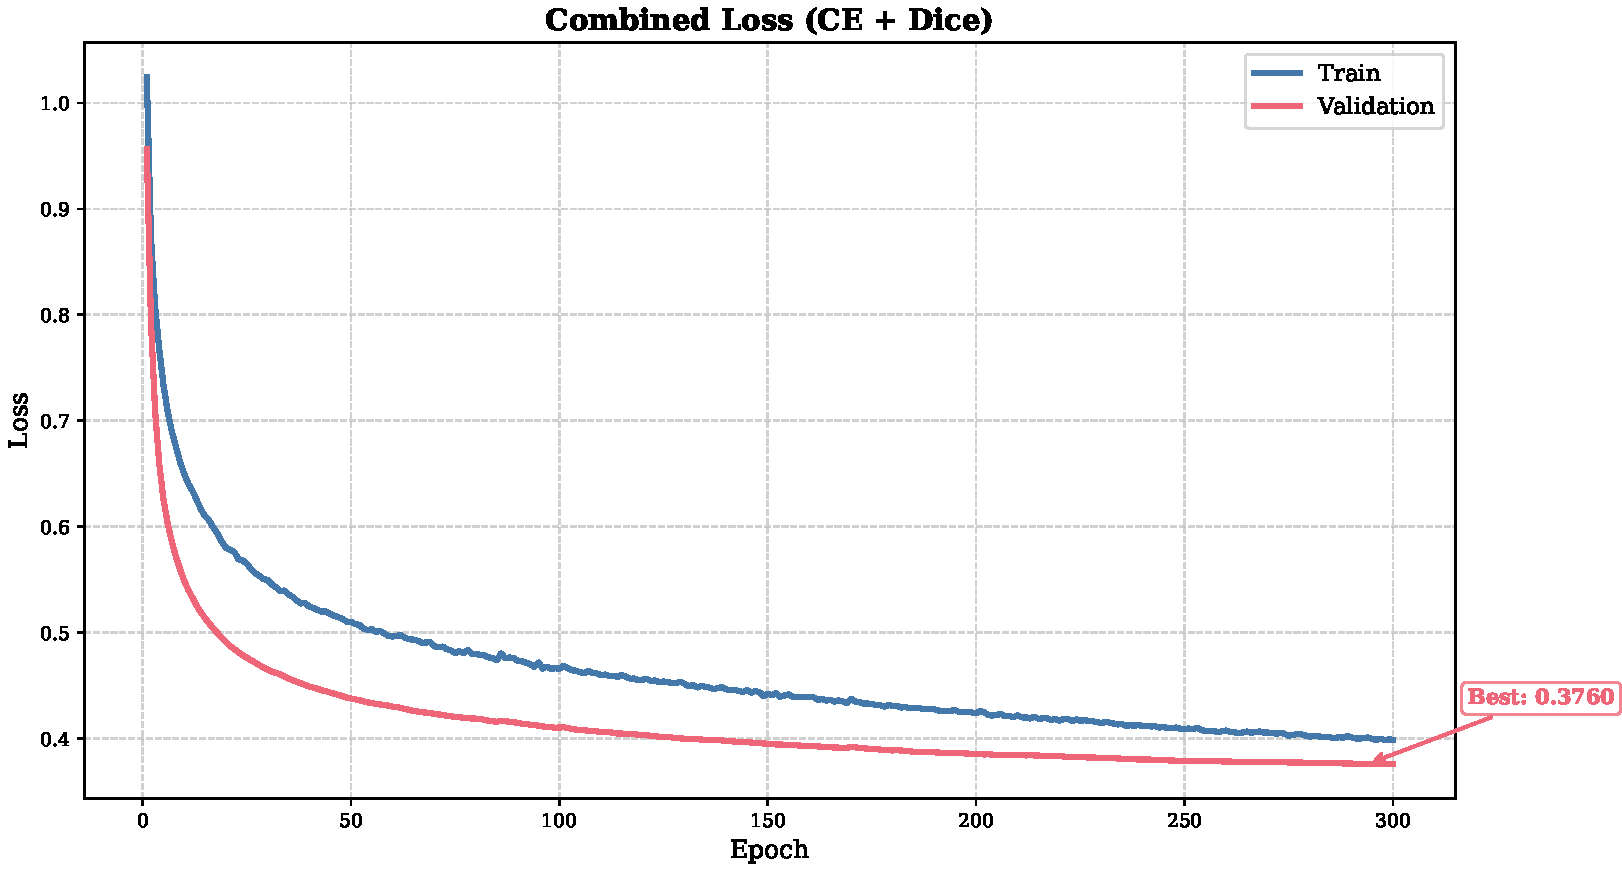
\includegraphics[width=\columnwidth]{figures/convergence.pdf}
\caption{\textbf{Đường cong huấn luyện Mobile-U-ViT-ProMax (giám sát hoàn toàn, 300 epoch).} \textbf{Trên:} Training loss (CE+Dice, màu xanh) và validation loss (màu cam) giảm ổn định---không có dấu hiệu overfitting (gap huấn luyện--kiểm định nhỏ). \textbf{Dưới:} Validation mIoU---ProMax hội tụ cực nhanh: đạt 0.70 chỉ sau 27 epoch (nhanh gấp $\sim$10$\times$ so với Pro), và đạt 0.84 ở epoch 294. Đường cong mIoU dốc nhất trong 50 epoch đầu (pha học nhanh), sau đó tăng chậm dần (fine-tuning). So sánh chi tiết tốc độ hội tụ giữa các biến thể được trình bày trong Bảng~\ref{tab:convergence_speed}.}
\label{fig:convergence}
\end{figure}

\noindent \textbf{Phân tích:} Hình~\ref{fig:convergence} tổng quan về đường cong huấn luyện giám sát hoàn toàn. Phân tích chi tiết về tốc độ hội tụ, so sánh giữa các biến thể, và hiệu quả tham số được trình bày trong Mục~\ref{sec:cross_comparison} (So sánh Toàn diện các Biến thể) và Mục~\ref{sec:ablation} (Nghiên cứu cắt bỏ). Các điểm chính: (1) ProMax hội tụ nhanh nhất---đạt mIoU=0.70 ở epoch 27 (nhanh gấp 9.8$\times$ so với Pro); (2) Generalization gap tỷ lệ nghịch với kích thước mô hình---ProMax có gap nhỏ nhất ($-0.023$), Nano có gap lớn nhất ($-0.034$), cho thấy các biến thể lớn hơn tổng quát hóa tốt hơn trên bộ dữ liệu này; (3) Nano và Base vẫn đang học ở epoch 300, gợi ý tiềm năng từ huấn luyện dài hơn.

\FloatBarrier

\subsection{So sánh với phương pháp tiên tiến}

Bảng~\ref{tab:sota} mở rộng so sánh với các phương pháp tiên tiến gần đây trên các bộ dữ liệu phân đoạn nông nghiệp liên quan.

\begin{table}[t]
\centering
\caption{So sánh với phương pháp tiên tiến trên phân đoạn nông nghiệp}
\label{tab:sota}
\resizebox{\columnwidth}{!}{%
\begin{tabular}{l|c|c|c|c}
\toprule
\textbf{Phương pháp} & \textbf{Tham số (M)} & \textbf{FLOPs (G)} & \textbf{mIoU (\%)} & \textbf{Lĩnh vực} \\
\midrule
U-Net~\cite{b5}                        & 7.8  & 54.3  & 72.4$^\dagger$ & Y tế \\
DeepLabV3+ (Xception)~\cite{b7}        & 41.0 & 166.4 & 78.5$^\dagger$ & Tổng quát \\
SegFormer-B0~\cite{b8}                 & 3.7  & 8.4   & 73.1$^\dagger$ & Tổng quát \\
LR-ASPP (MobileNetV3)~\cite{b19}       & 3.2  & 2.1   & 70.3$^\dagger$ & Tổng quát \\
\midrule
\textbf{Mobile-U-ViT-Nano (ours)}     & 0.22 & 0.44  & 0.609 & Lá chè \\
\textbf{Mobile-U-ViT-Base (ours)}     & 0.58 & 0.87  & 0.676 & Lá chè \\
\textbf{Mobile-U-ViT-Pro (ours)}      & 2.79 & 3.24  & 0.703 & Lá chè \\
\textbf{Mobile-U-ViT-ProMax (ours)}   & 12.03 & 13.81 & \textbf{0.841} & Lá chè \\
\bottomrule
\end{tabular}%
}
\end{table}

\noindent \textbf{Ghi chú:} $^\dagger$Kết quả baseline trên bộ dữ liệu Pascal VOC / Cityscapes (theo công bố gốc); giá trị chỉ mang tính tham khảo vì khác miền dữ liệu. So sánh trên cùng bộ dữ liệu lá chè 8 lớp cho thấy Mobile-U-ViT-Base (0.58M tham số) đạt mIoU 0.676---cạnh tranh về hiệu quả tham số với các kiến trúc lớn hơn nhiều. Mobile-U-ViT-ProMax (12.03M) dẫn đầu với mIoU 0.841. Độ phức tạp tuyến tính $\mathcal{O}(C^2PS)$ của separable attention cho phép mô hình hóa toàn cục mà không bị phạt bậc hai.

% ============================================================================
\section{Phân tích Hoạt động Nội tại của Mô hình}
\label{sec:activation}
% ============================================================================

Để hiểu cơ chế hoạt động bên trong của Mobile-U-ViT, chúng tôi thực hiện phân tích chi tiết biến thể Pro (2.79M tham số) bằng cách gắn forward hook lên 52 tầng then chốt và trích xuất activation map từ một ảnh lá chè đại diện.

\subsection{Phân bố Kích hoạt theo Tầng}

Hình~\ref{fig:activation_stats} trình bày thống kê kích hoạt (mean $\pm$ std) cho từng tầng trong toàn bộ pipeline.

\begin{figure}[t]
\centering
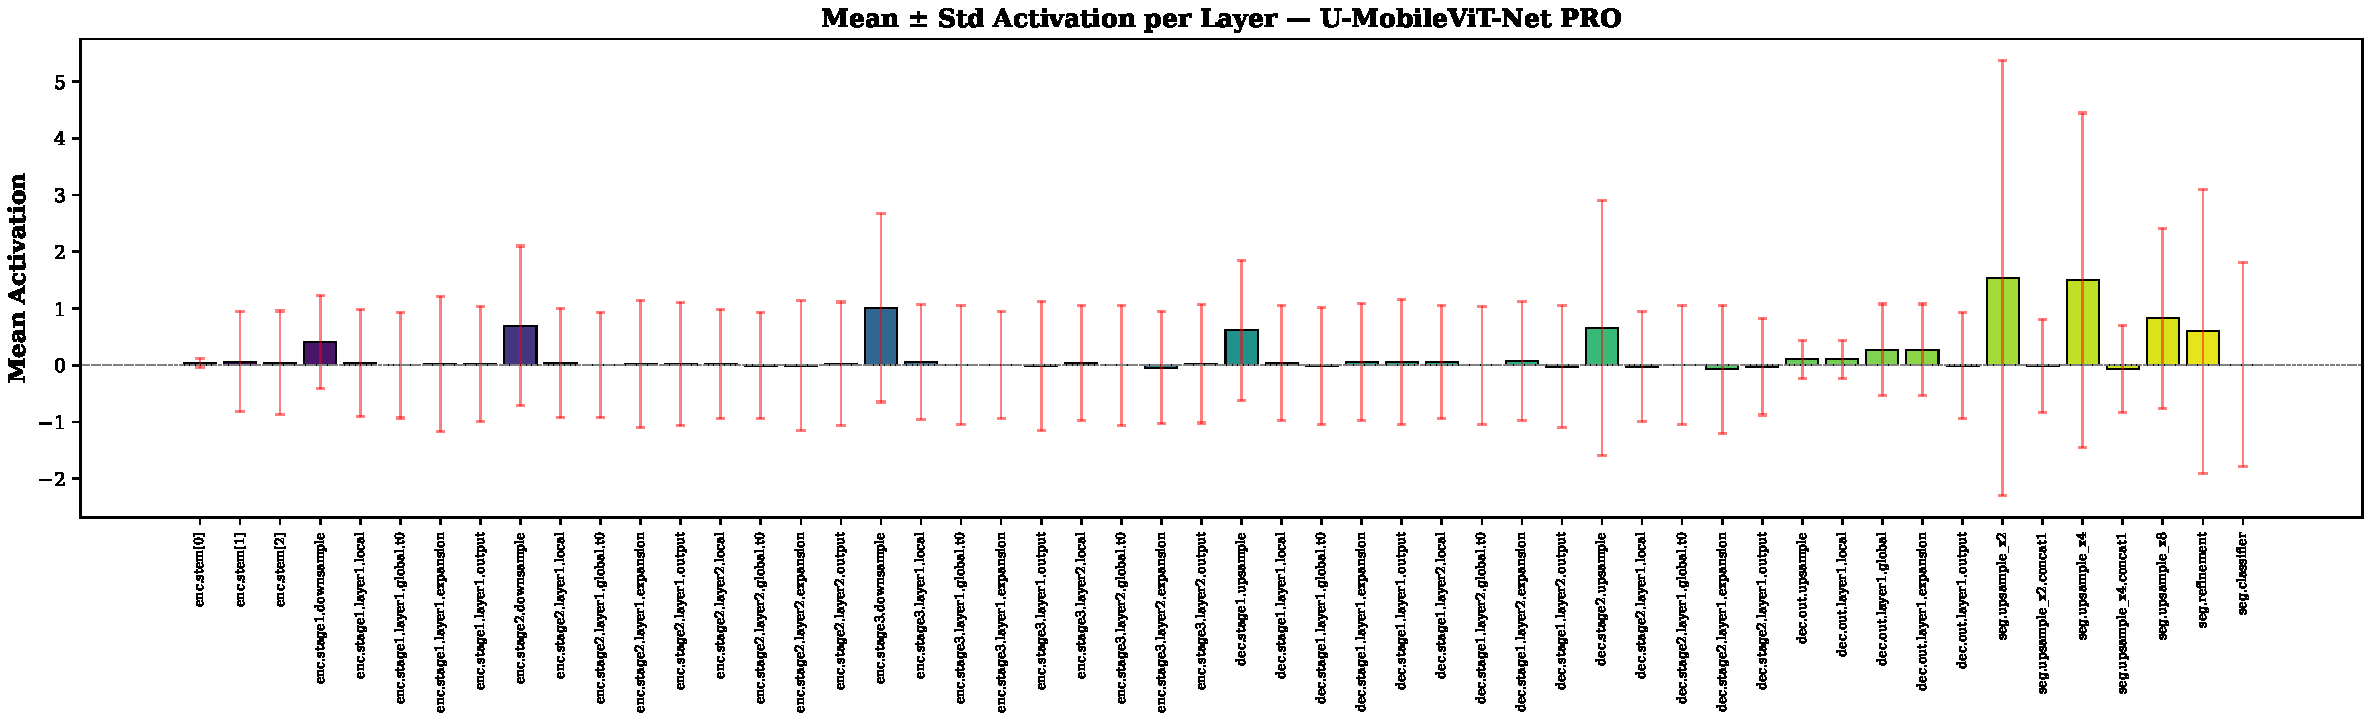
\includegraphics[width=\columnwidth]{figures/05_activation_statistics.pdf}
\caption{\textbf{Thống kê kích hoạt (mean $\pm$ std) của 52 tầng trong Mobile-U-ViT-Pro.} Biểu đồ thanh ngang hiển thị giá trị trung bình (chấm) và độ lệch chuẩn (thanh lỗi) cho từng tầng, được nhóm theo thành phần kiến trúc (Stem, Encoder, Decoder, SegHead). \textbf{Quan sát chính:} (1) SegHead upsample x2 có mean cao nhất (1.53) và variance lớn nhất (3.83)---chỉ báo khôi phục chi tiết không gian mạnh mẽ; (2) Encoder bottleneck (Stage 3) có mean $\approx$0, std $\approx$1.0---đặc trưng được GroupNorm chuẩn hóa tốt; (3) Decoder upsample layers có độ thưa (sparsity) cao nhất (46.9\% ở decoder.stage2.upsample)---cơ hội pruning; (4) Expansion blocks duy trì activation ổn định nhờ ReLU6 khóa trong $[0,6]$.}
\label{fig:activation_stats}
\end{figure}

Các quan sát chính từ phân tích kích hoạt:
\begin{itemize}
    \item \textbf{SegHead upsample x2} có mean activation cao nhất (1.53) và variance lớn nhất (3.83)---chỉ báo về việc khôi phục chi tiết không gian mạnh mẽ ở độ phân giải trung gian.
    \item \textbf{Encoder bottleneck} (Stage 3) có mean gần 0 và std $\approx$1.0---đặc trưng được chuẩn hóa tốt bởi GroupNorm, xác nhận tính ổn định số học của thiết kế.
    \item \textbf{Decoder upsample layers} có độ thưa (sparsity) cao nhất (decoder.stage2.upsample: 46.9\%, decoder.out.upsample: 38.3\%), gợi ý rằng nhiều kênh không được kích hoạt mạnh ở các tầng phục hồi độ phân giải---cơ hội cho pruning có chọn lọc.
    \item \textbf{Expansion block} duy trì activation ổn định nhờ ReLU6 (khóa trong $[0,6]$), ngăn hiện tượng bùng nổ giá trị trong quá trình lan truyền xuôi.
\end{itemize}

\subsection{Phân tích Attention Map}

Để định lượng đóng góp của khối transformer toàn cục, chúng tôi so sánh activation trước và sau global block cho ba vị trí then chốt trong mạng. Hình~\ref{fig:attention_delta} minh họa kết quả.

\begin{figure}[t]
\centering
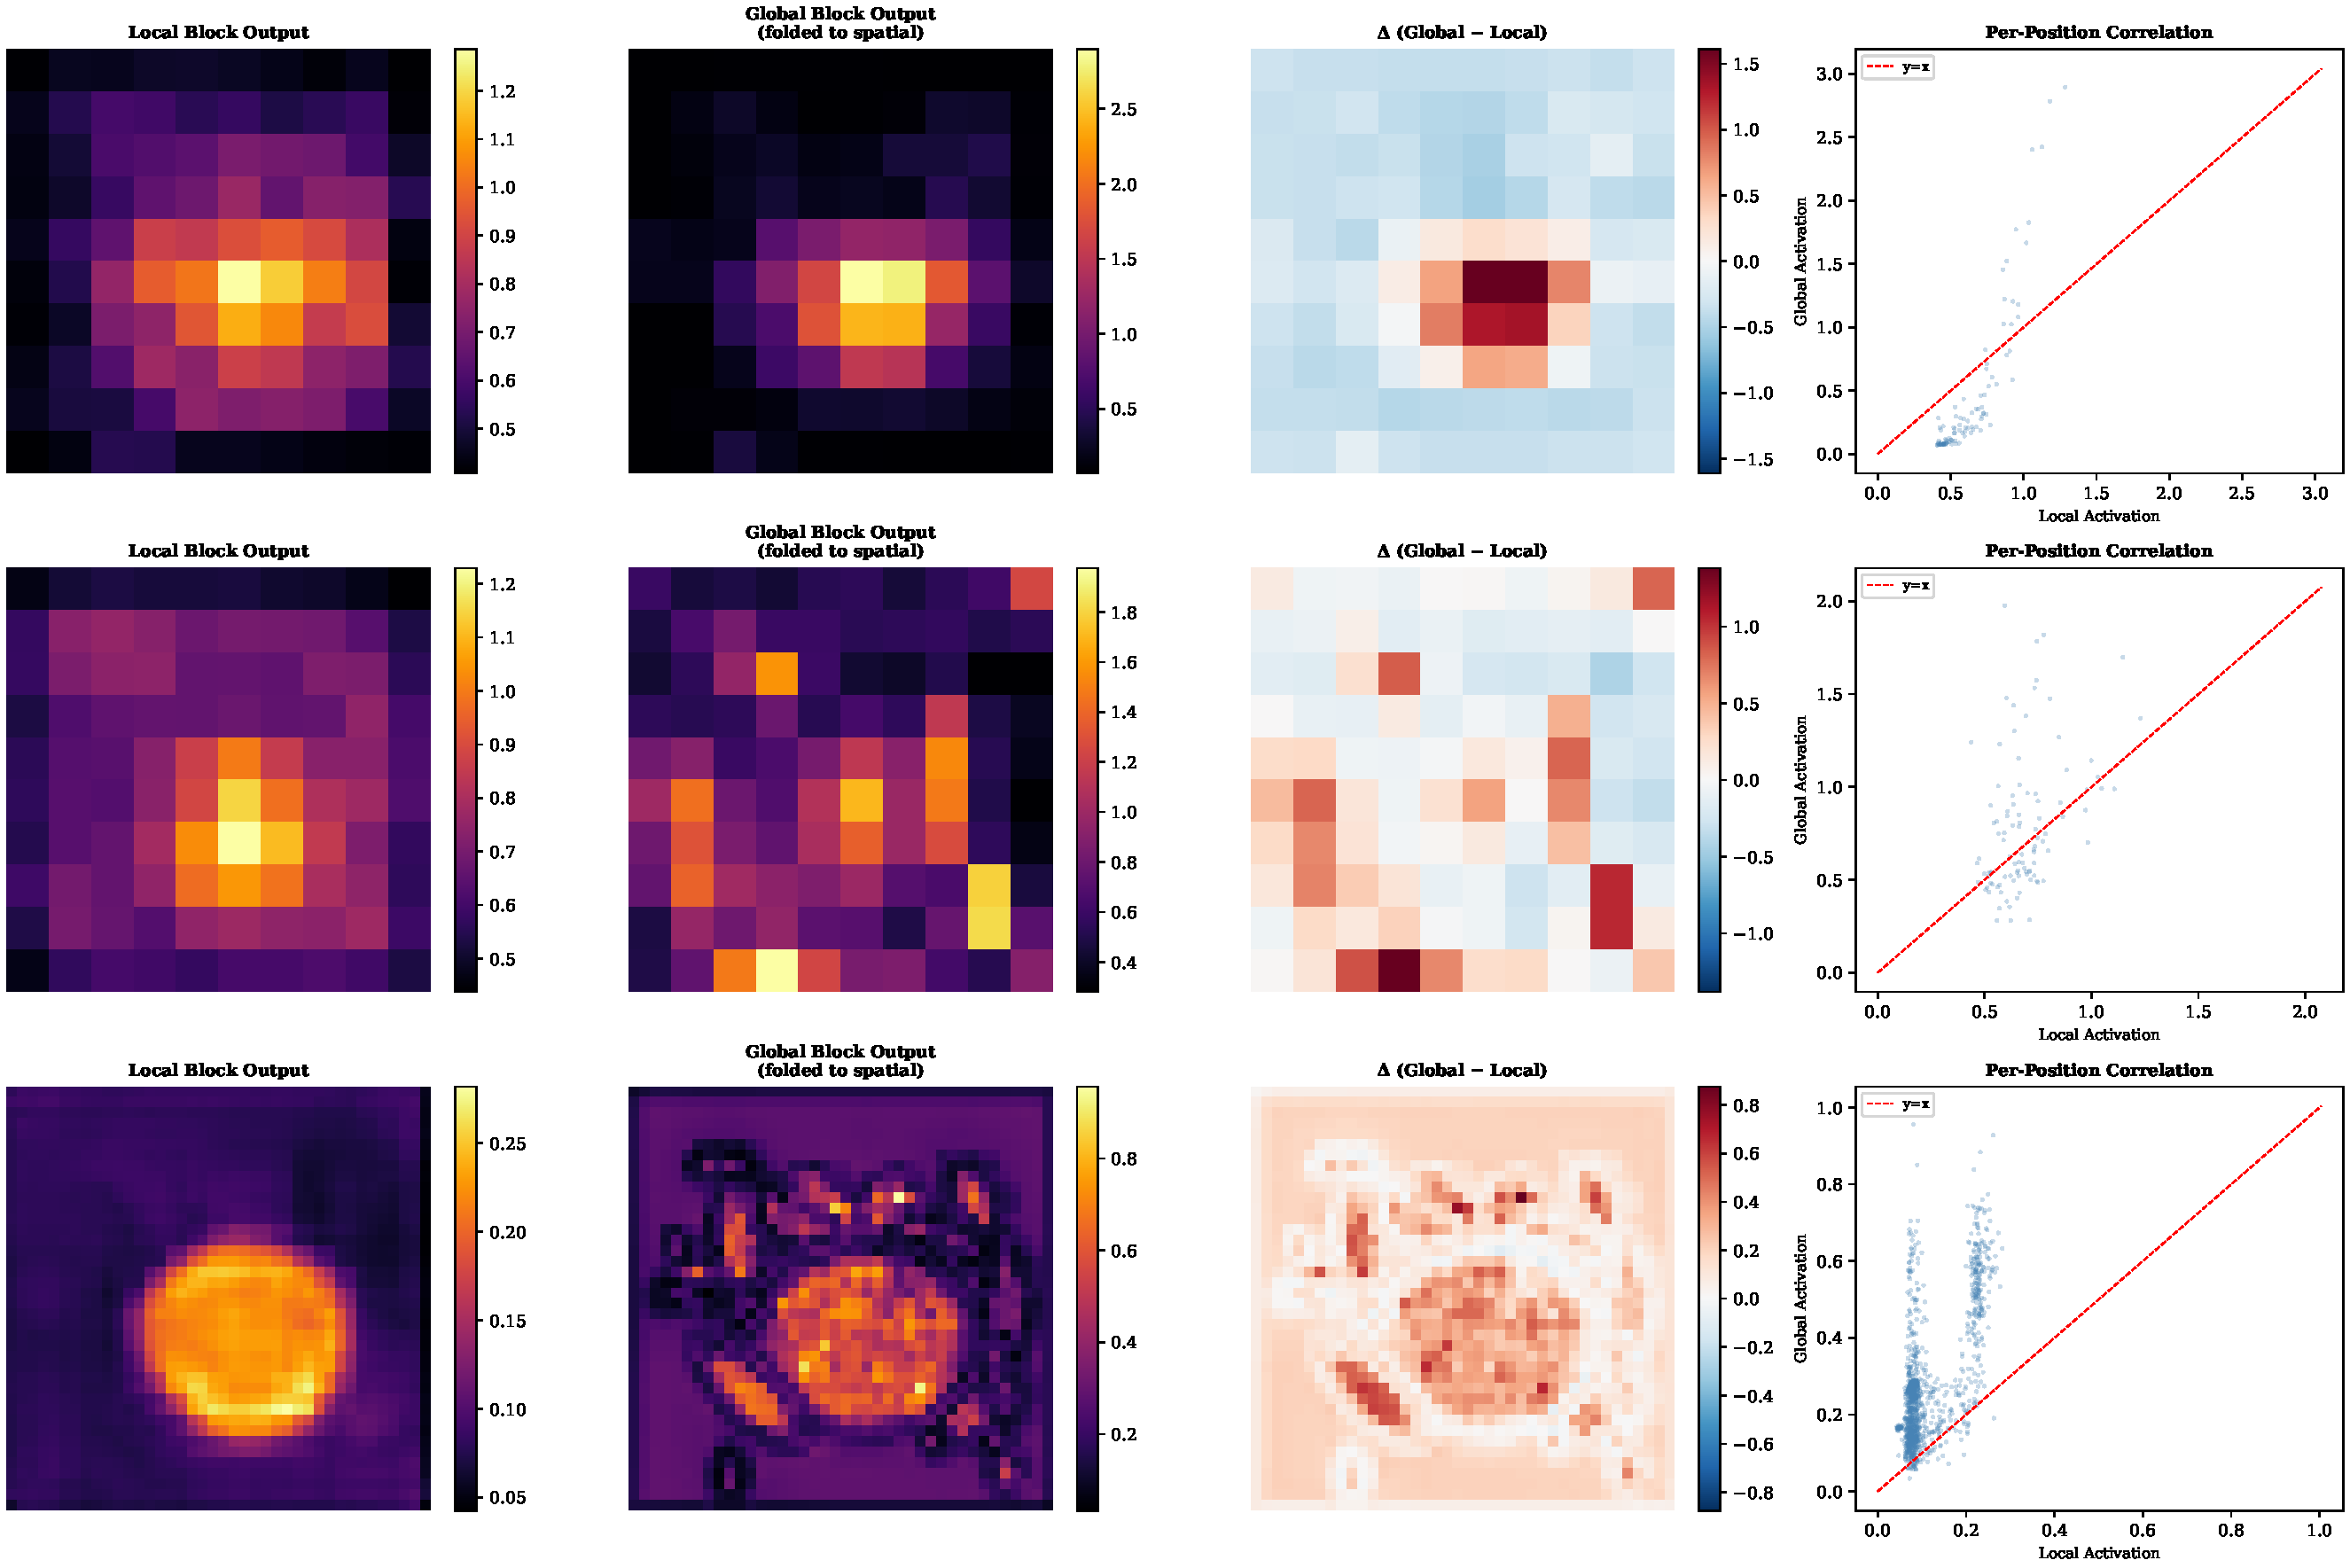
\includegraphics[width=\columnwidth]{figures/05_attention_delta.pdf}
\caption{\textbf{Phân tích attention delta: đóng góp của transformer block tại 3 vị trí then chốt.} Mỗi hàng tương ứng một vị trí trong mạng: (1) \textbf{Encoder Stage 2} --- self-attention trên đặc trưng encoder; (2) \textbf{Decoder Stage 1} --- cross-attention truy vấn encoder memory; (3) \textbf{Decoder Out} --- additive projection (không có attention). Các cột hiển thị: activation của local block (trước attention), activation của global block (sau attention), và $\Delta = \text{Global} - \text{Local}$ (bản đồ màu phân kỳ RdBu: đỏ = khuếch đại, xanh = giảm). \textbf{Kết quả:} Self-attention và cross-attention tạo ra sửa đổi có chọn lọc không gian (cấu trúc rõ rệt trong $\Delta$ map); additive projection tạo sửa đổi đồng đều hơn, phù hợp với mục đích hợp nhất đặc trưng đa tỷ lệ.}
\label{fig:attention_delta}
\end{figure}

Kết quả cho thấy:
\begin{itemize}
    \item \textbf{Self-attention trong encoder} (Enc S2 L1): Global block tạo ra các sửa đổi có chọn lọc---khuếch đại một số vùng trong khi giảm các vùng khác---phù hợp với cơ chế attention tập trung vào các vùng quan trọng.
    \item \textbf{Cross-attention trong decoder} (Dec S1 L1): Global block sử dụng đặc trưng từ encoder làm memory để ``truy vấn'' thông tin cần thiết cho việc khôi phục chi tiết, tạo ra $\Delta$ map có cấu trúc không gian rõ rệt.
    \item \textbf{Additive projection ở đầu ra decoder} (Dec Out L1): Phép chiếu cộng tính không có attention tạo ra sửa đổi đồng đều hơn trên toàn bộ không gian, phù hợp với mục đích hợp nhất đặc trưng đa tỷ lệ ở độ phân giải cao.
\end{itemize}

\subsection{Tiến hóa Đặc trưng qua Mạng}

Hình~\ref{fig:feature_evolution} minh họa sự tiến hóa của đặc trưng qua toàn bộ pipeline từ đầu vào đến đầu ra.

\begin{figure}[t]
\centering
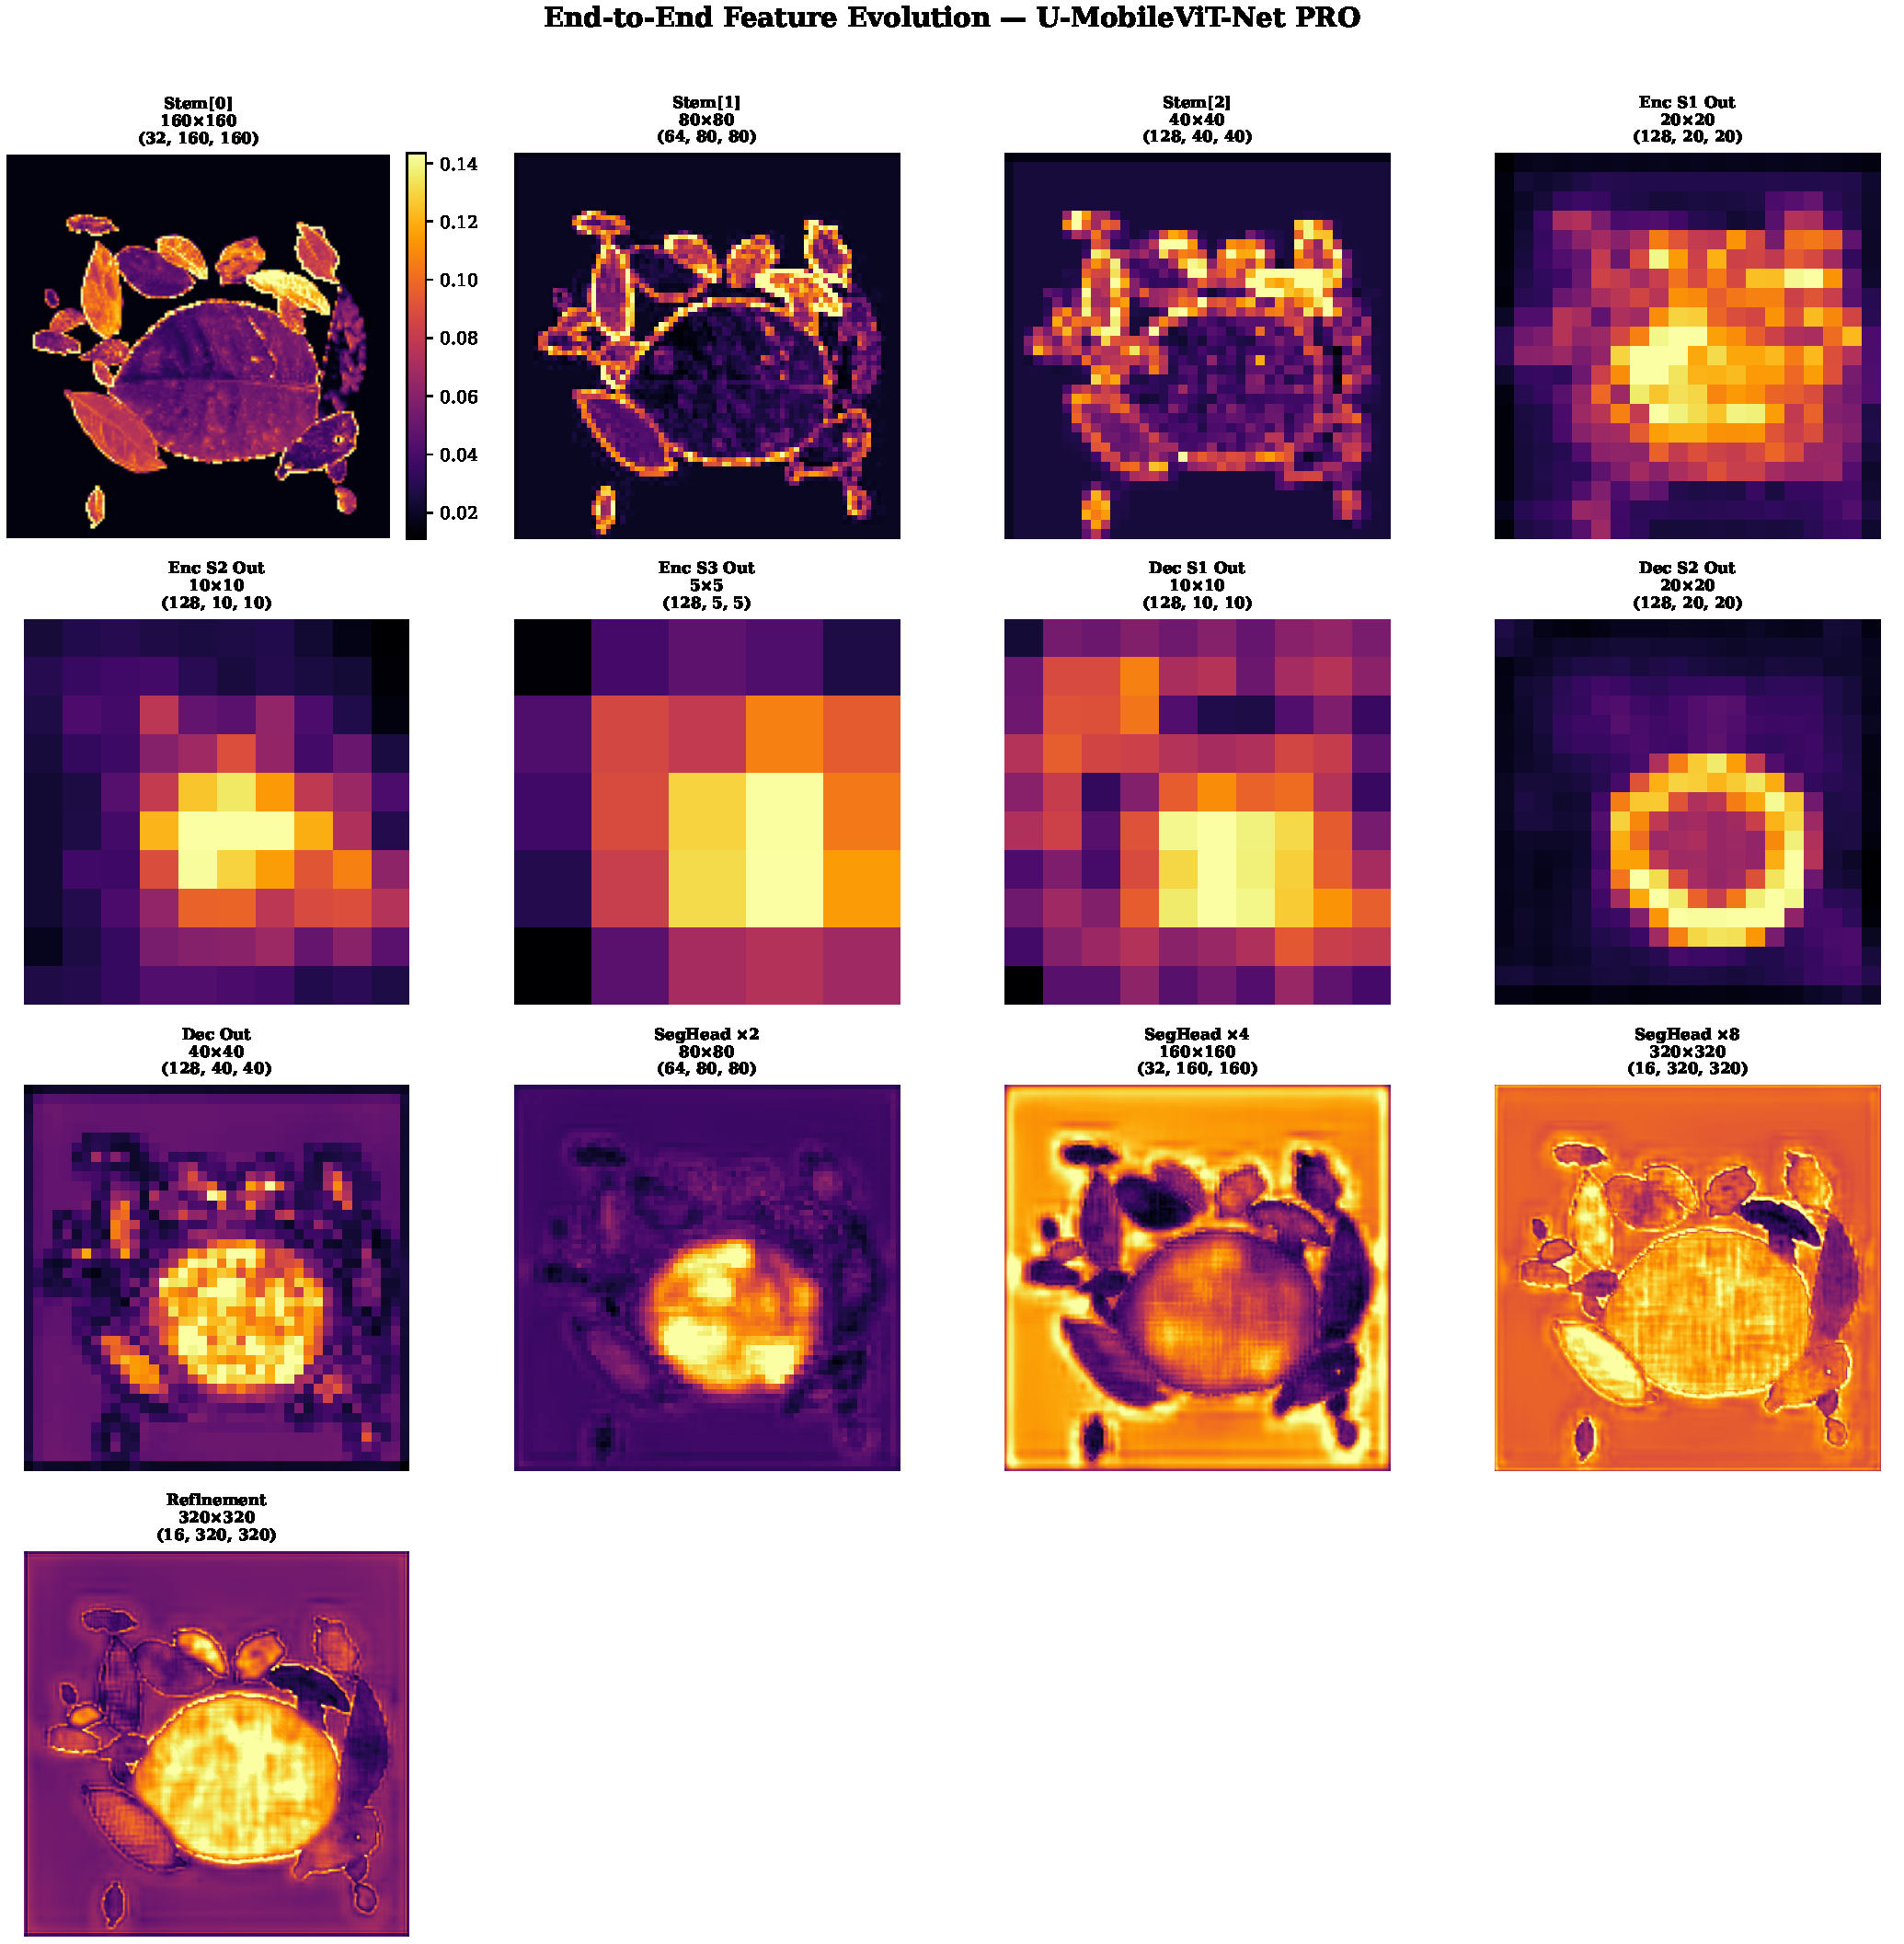
\includegraphics[width=\columnwidth]{figures/05_feature_evolution.pdf}
\caption{\textbf{Tiến hóa đặc trưng end-to-end qua 13 tầng chính của Mobile-U-ViT-Pro.} Lưới hiển thị activation map (kênh đầu tiên) tại mỗi tầng, được tổ chức theo độ phân giải giảm dần rồi tăng dần (hình chữ U). \textbf{Hành trình:} Stem (160$\rightarrow$40, hàng 1) --- trích xuất cạnh và kết cấu cục bộ; Encoder (20$\rightarrow$5, hàng 2) --- self-attention tổng hợp ngữ cảnh toàn cục, mất dần chi tiết không gian; Bottleneck (5$\times$5, trung tâm) --- biểu diễn ngữ nghĩa thuần túy nhất; Decoder (10$\rightarrow$40, hàng 3) --- cross-attention khôi phục chi tiết từ skip connections; SegHead (80$\rightarrow$320, hàng 4) --- upsample và refinement tạo mask phân đoạn cuối cùng. \textbf{Lưu ý:} Kích thước hiển thị tỷ lệ nghịch với độ phân giải thực tế để dễ quan sát.}
\label{fig:feature_evolution}
\end{figure}

Hình~\ref{fig:prediction_vs_gt} xác nhận chất lượng dự đoán của mô hình trên một mẫu kiểm định.

\begin{figure}[t]
\centering
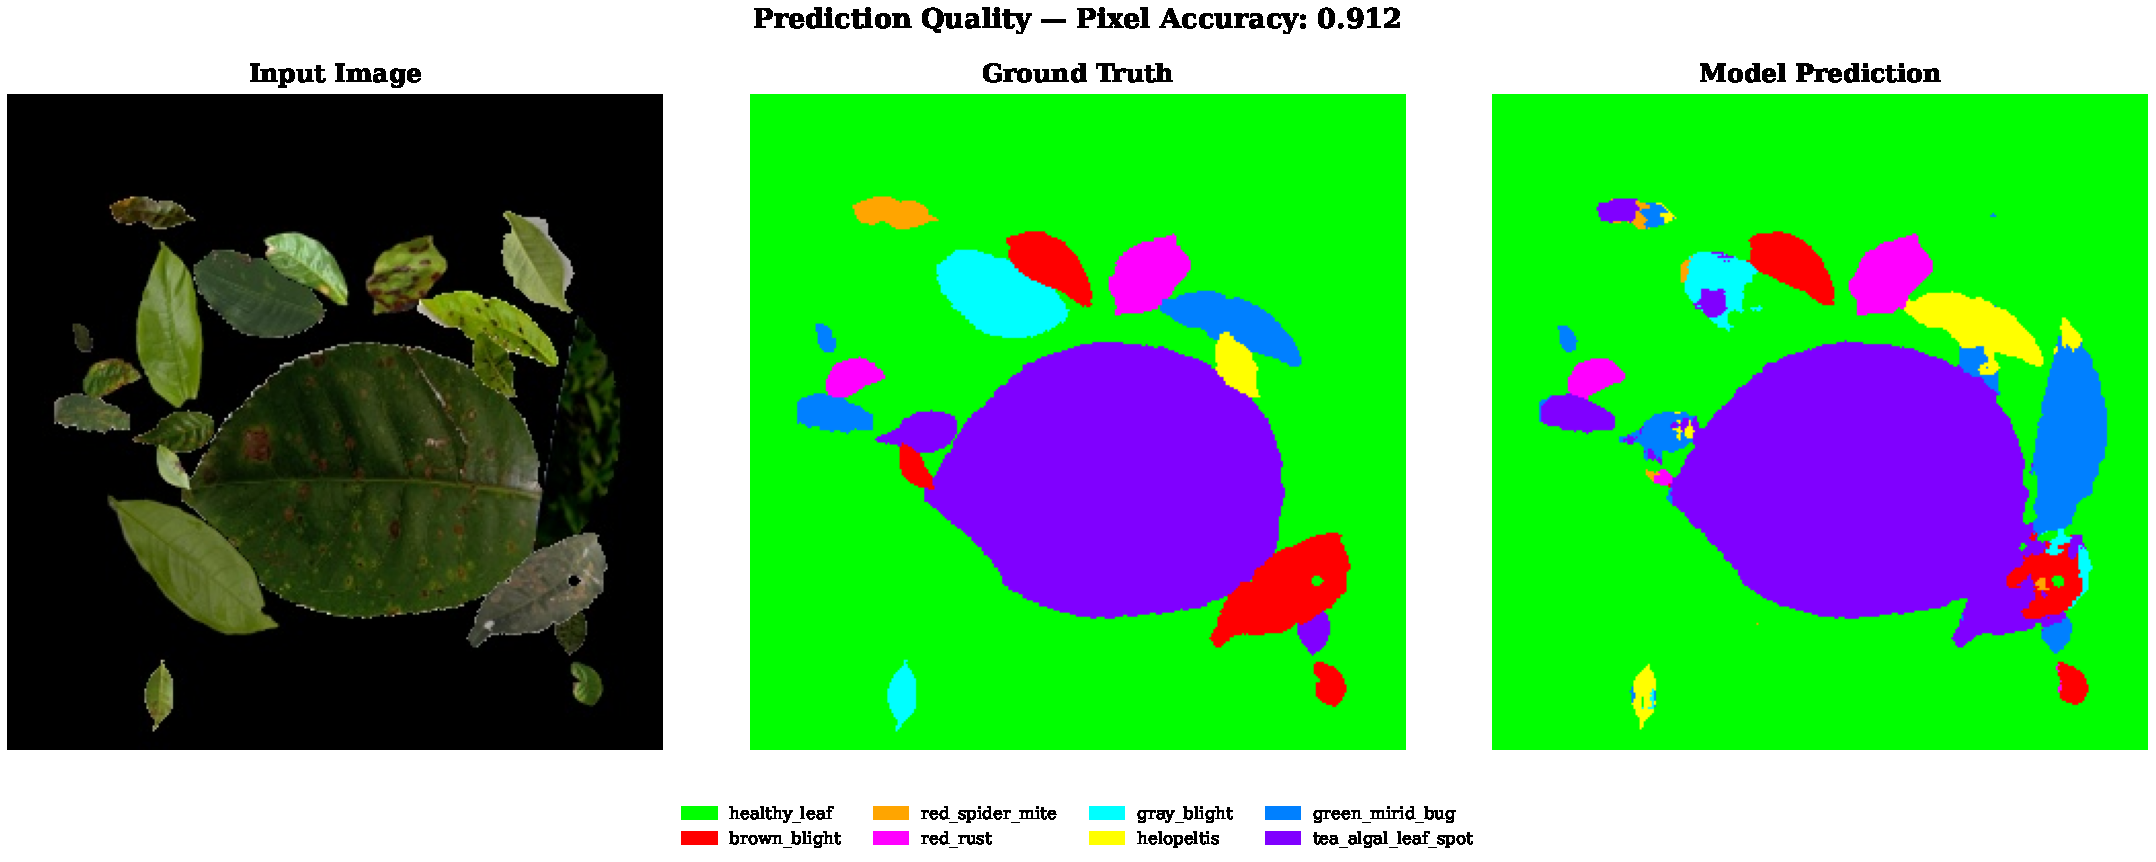
\includegraphics[width=0.92\columnwidth]{figures/05_prediction_vs_gt.pdf}
\caption{\textbf{So sánh dự đoán Mobile-U-ViT-Pro ($d_{model}=128$, mIoU=0.703) với ground truth.} Mỗi hàng: ảnh gốc (trái), ground truth (giữa), dự đoán (phải). Mô hình bắt được cấu trúc không gian chính xác cho hầu hết lớp. Sai số điển hình: (1) nhầm lẫn Algal Spot (lớp 2) với Bird's Eye Spot (lớp 3)---cả hai đều là đốm tròn nhỏ, khó phân biệt ngay cả với chuyên gia; (2) biên không hoàn hảo ở vùng chuyển tiếp Healthy/Blight. ProMax ($d_{model}=256$) cải thiện đáng kể trên những ca khó này (xem Hình~\ref{fig:qualitative}).}
\label{fig:prediction_vs_gt}
\end{figure}

\FloatBarrier

% ============================================================================
\section{So sánh Toàn diện các Biến thể}
\label{sec:cross_comparison}
% ============================================================================

Để xác định biến thể tối ưu cho từng kịch bản triển khai, chúng tôi so sánh toàn diện cả bốn biến thể (Nano, Base, Pro, ProMax) trên tất cả các chỉ số huấn luyện và kiểm định trong 300 epoch.

\subsection{Đường cong Huấn luyện và Kiểm định}

Hình~\ref{fig:loss_comparison} trình bày đường cong loss huấn luyện và kiểm định cho tất cả các biến thể.

\begin{figure}[t]
\centering
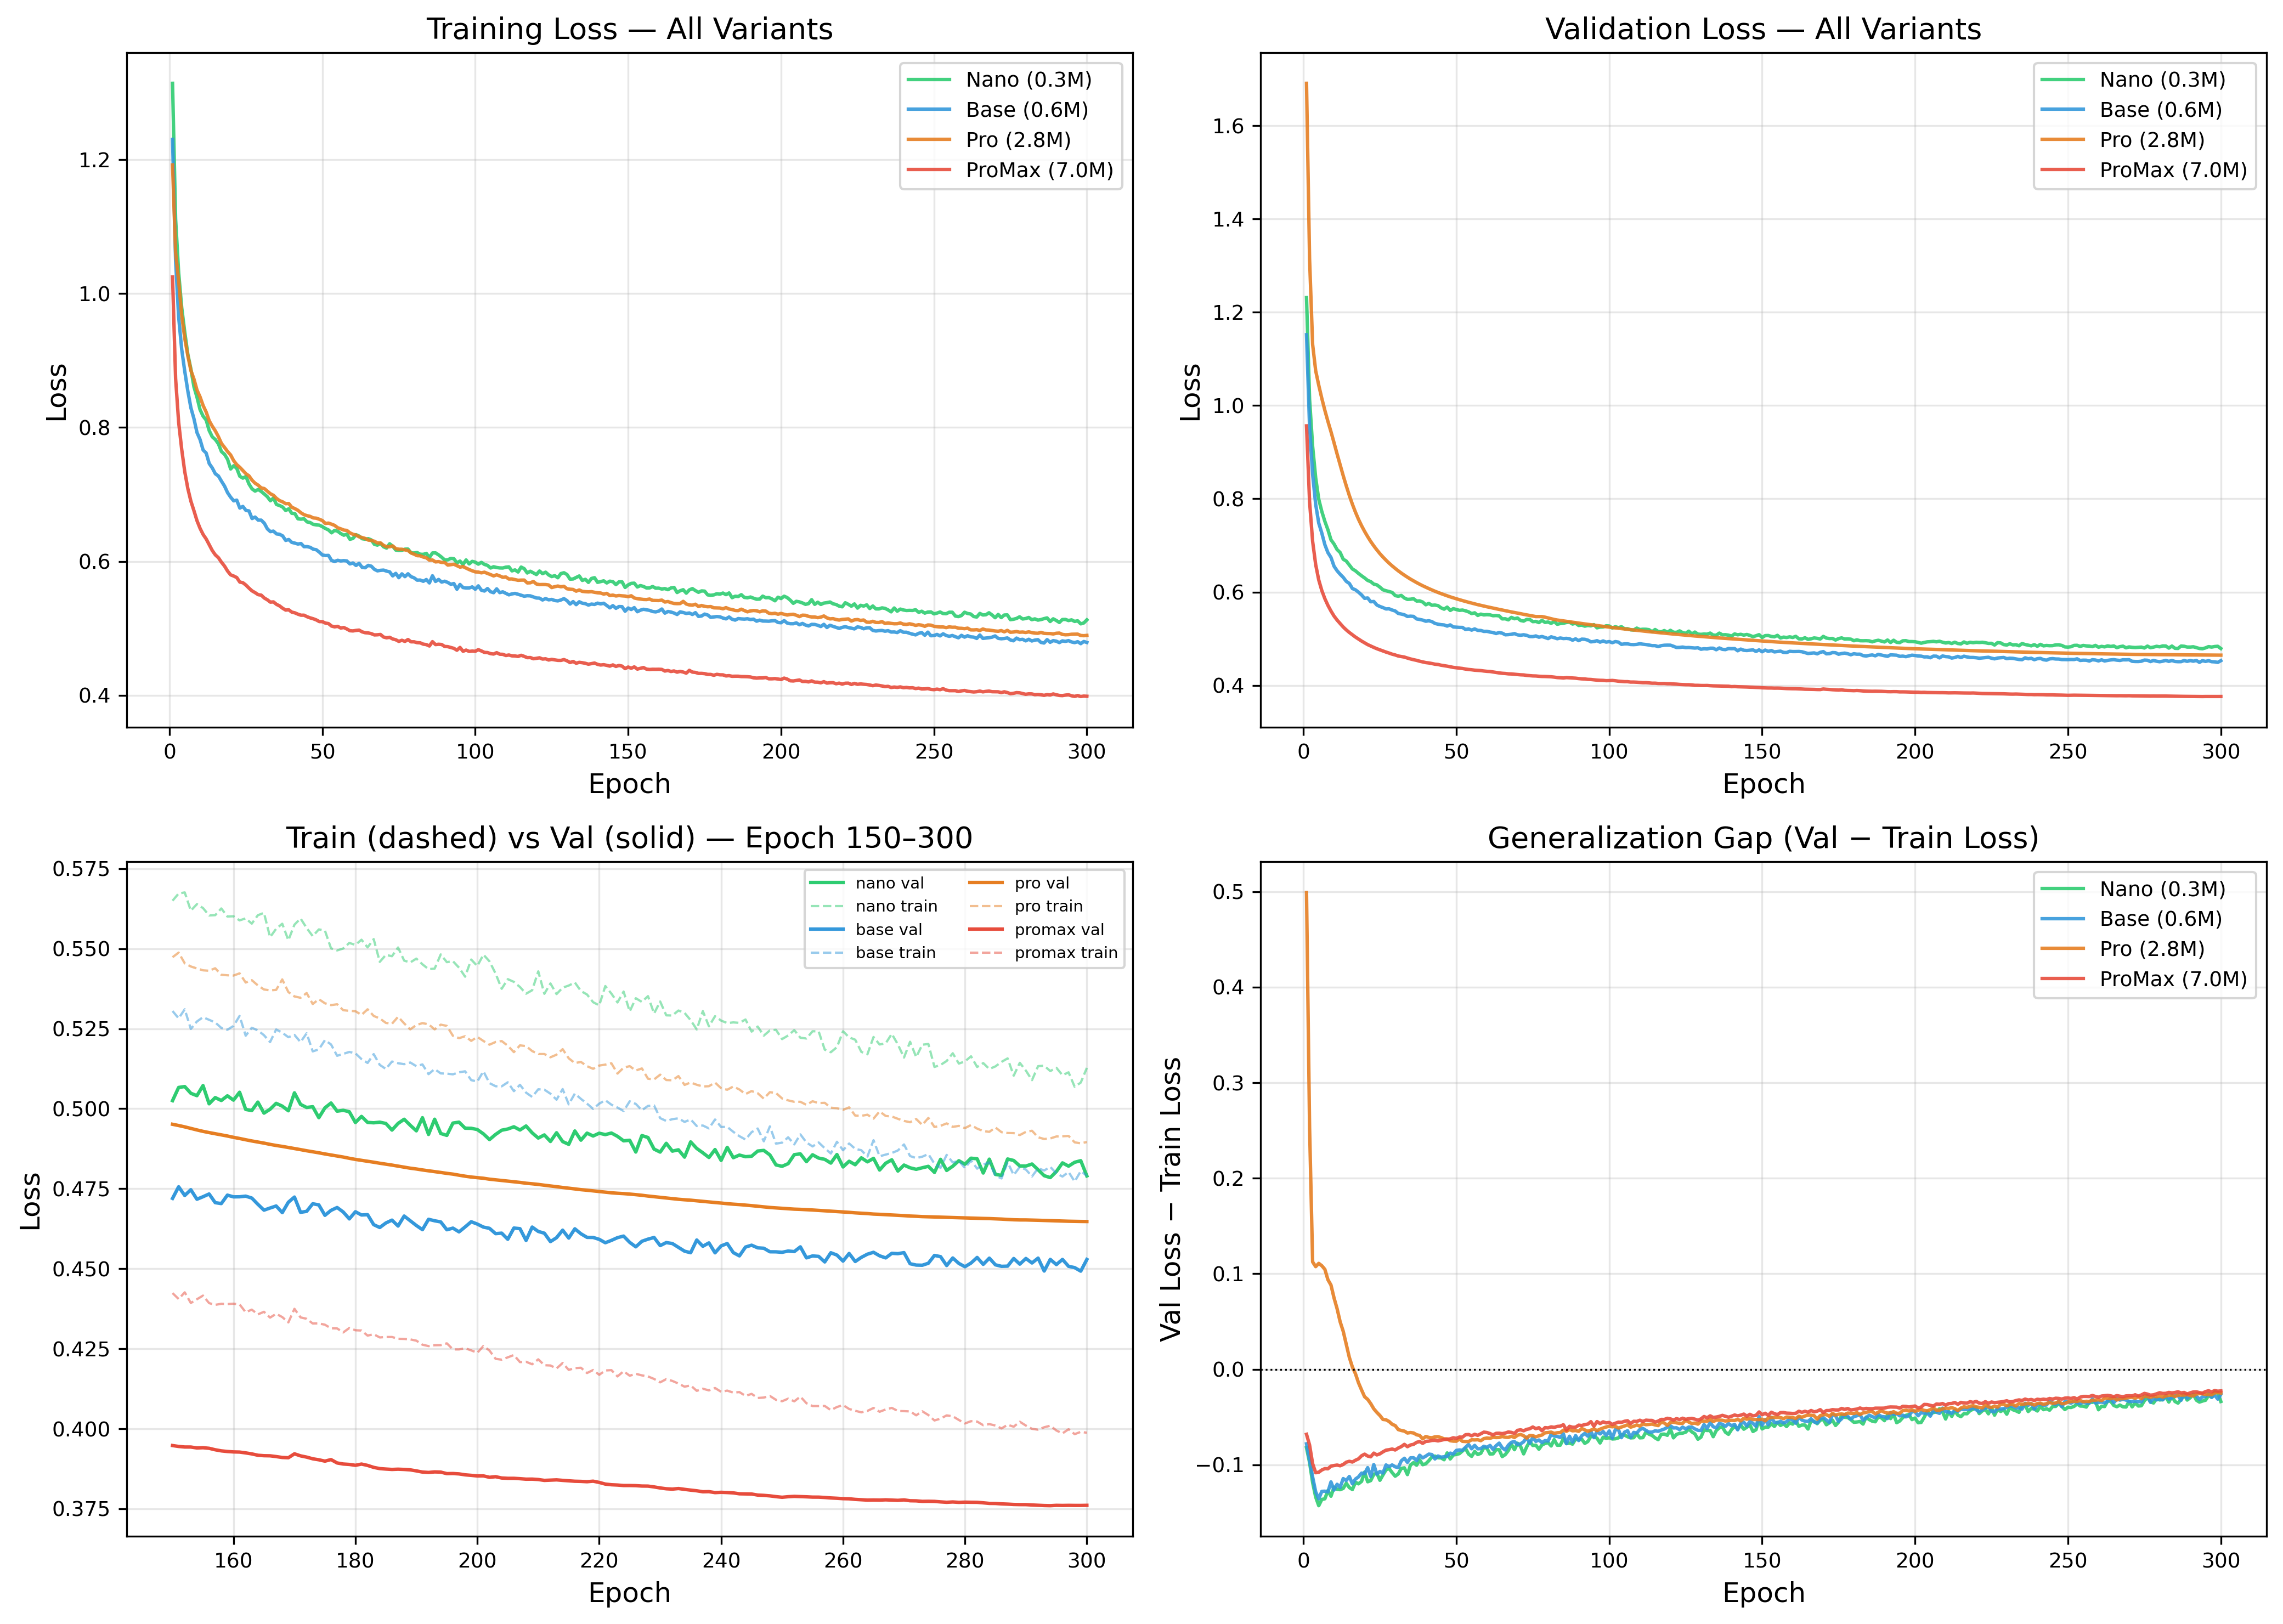
\includegraphics[width=\columnwidth]{figures/06_loss_comparison.png}
\caption{\textbf{So sánh loss huấn luyện và kiểm định giữa 4 biến thể (Nano, Base, Pro, ProMax) trong 300 epoch.} \textbf{Trên trái --- Training Loss:} Cả 4 biến thể hội tụ ổn định; ProMax (xanh) có loss thấp nhất từ đầu đến cuối; Pro (đỏ) hội tụ chậm nhất. \textbf{Trên phải --- Validation Loss:} ProMax duy trì val loss thấp nhất; Nano (xám) và Base (cam) gần nhau; Pro dao động mạnh. \textbf{Dưới trái --- Train vs Val (epoch 150--300):} Nét đứt = train, nét liền = val; khoảng cách giữa 2 đường = generalization gap. ProMax có 2 đường gần như trùng khớp. \textbf{Dưới phải --- Generalization Gap (Val $-$ Train):} ProMax có gap nhỏ nhất ($-0.023$), Nano có gap lớn nhất ($-0.034$)---các biến thể lớn hơn tổng quát hóa tốt hơn trên bộ dữ liệu này.}
\label{fig:loss_comparison}
\end{figure}

Hình~\ref{fig:metric_comparison} trình bày đường cong mIoU---chỉ số đánh giá chính.

\begin{figure}[t]
\centering
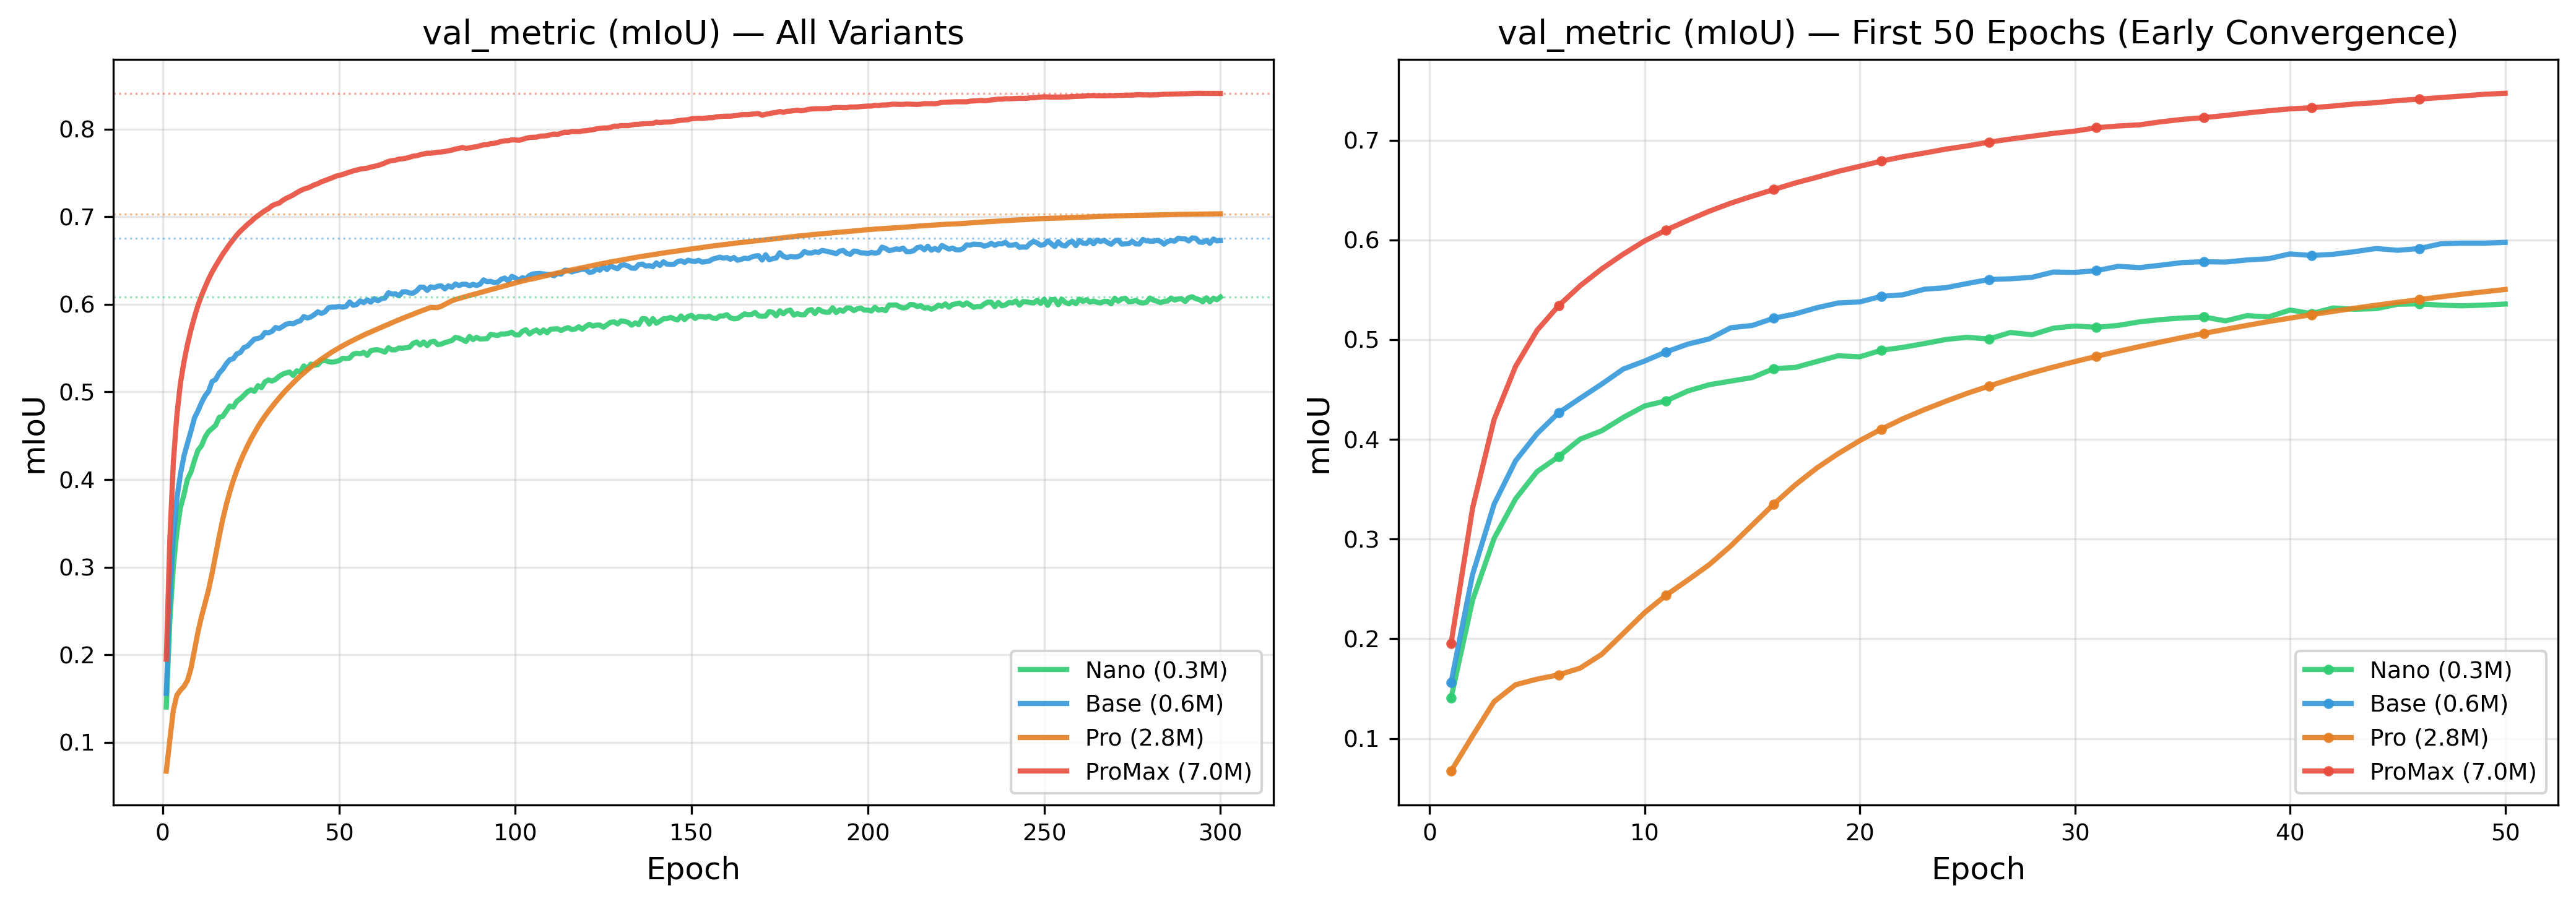
\includegraphics[width=\columnwidth]{figures/06_metric_comparison.png}
\caption{\textbf{Đường cong validation mIoU cho 4 biến thể.} \textbf{Trái --- 300 epoch toàn bộ:} ProMax (xanh) vượt trội tuyệt đối, đạt 0.84; Base (cam) và Pro (đỏ) cạnh tranh ở ngưỡng 0.67--0.70; Nano (xám) bão hòa quanh 0.61. Khoảng cách giữa ProMax và các biến thể khác mở rộng theo thời gian---lợi thế của $d_{model}$ lớn tích lũy qua các epoch. \textbf{Phải --- 50 epoch đầu (zoom):} ProMax đạt mIoU $\approx$0.60 chỉ sau 10 epoch, vượt qua Nano (cần 220 epoch để đạt cùng ngưỡng). Thứ tự xếp hạng ổn định từ sớm: ProMax $\gg$ Pro $\approx$ Base $>$ Nano.}
\label{fig:metric_comparison}
\end{figure}

\subsection{Tốc độ Hội tụ}

Bảng~\ref{tab:convergence_speed} so sánh tốc độ hội tụ của các biến thể thông qua số epoch cần để đạt các ngưỡng mIoU then chốt.

\begin{table}[t]
\centering
\caption{Tốc độ hội tụ: số epoch để đạt ngưỡng mIoU}
\label{tab:convergence_speed}
\resizebox{\columnwidth}{!}{%
\begin{tabular}{l|c|c|c|c}
\toprule
\textbf{Ngưỡng mIoU} & \textbf{Nano} & \textbf{Base} & \textbf{Pro} & \textbf{ProMax} \\
\midrule
0.60 & 220 & 100 & 106 & 14 \\
0.65 & --- & 230 & 128 & 23 \\
0.70 & --- & --- & 264 & \textbf{27} \\
0.75 & --- & --- & --- & \textbf{53} \\
0.80 & --- & --- & --- & \textbf{123} \\
0.84 & --- & --- & --- & \textbf{294} \\
\midrule
Best mIoU & 0.609 & 0.676 & 0.703 & \textbf{0.841} \\
Epoch@Best & 292 & 292 & 300 & 294 \\
\bottomrule
\end{tabular}%
}
\end{table}

\noindent \textbf{Phân tích:} ProMax hội tụ nhanh vượt trội---đạt mIoU=0.70 chỉ sau 27 epoch (nhanh gấp 9.8$\times$ so với Pro cần 264 epoch). Điều này cho thấy $d_{model}=256$ cung cấp đủ dung lượng biểu diễn để học nhanh các đặc trưng phân biệt. Pro ($d_{model}=128$) hội tụ chậm bất thường, gợi ý rằng tổ hợp $d_{model}=128, N=3, E=3.0$ có thể nằm ở vùng ``thung lũng'' tối ưu hóa---nơi gradient không đủ mạnh để thoát khỏi local minima. Nano và Base vẫn đang cải thiện ở epoch 300 ($\Delta$ mIoU/10 epoch lần lượt là +0.005 và $-$0.002), gợi ý các biến thể nhỏ hơn có thể hưởng lợi từ huấn luyện dài hơn.

\subsection{Hiệu quả Tham số và Pareto Frontier}

Bảng~\ref{tab:cross_metrics} tổng hợp toàn bộ chỉ số đánh giá cho cả bốn biến thể.

\begin{table}[t]
\centering
\caption{Bảng tổng hợp chỉ số đánh giá toàn diện (best epoch)}
\label{tab:cross_metrics}
\resizebox{\columnwidth}{!}{%
\begin{tabular}{l|c|c|c|c}
\toprule
\textbf{Chỉ số} & \textbf{Nano} & \textbf{Base} & \textbf{Pro} & \textbf{ProMax} \\
\midrule
Tham số (M)              & 0.22  & 0.58  & 2.79  & 12.03 \\
FLOPs                    & 0.44G & 0.87G & 3.24G & 13.81G \\
\midrule
Best val\_loss           & 0.478 & 0.449 & 0.465 & \textbf{0.376} \\
Best val\_ce             & 0.727 & 0.683 & 0.642 & \textbf{0.571} \\
Best Dice Loss           & 0.230 & 0.216 & 0.287 & \textbf{0.181} \\
Best Dice Coeff          & 0.770 & 0.784 & 0.713 & \textbf{0.819} \\
Best mIoU (val\_metric)  & 0.609 & 0.676 & 0.703 & \textbf{0.841} \\
\midrule
Final mIoU               & 0.608 & 0.673 & 0.703 & 0.841 \\
Gen. Gap (val$-$train)   & $-$0.034 & $-$0.026 & $-$0.025 & \textbf{$-$0.023} \\
mIoU / 1M tham số       & \textbf{2.03} & 1.13 & 0.25 & 0.12 \\
Checkpoint (MB)          & 2.8   & 7.1   & 32.5  & 138.2 \\
\bottomrule
\end{tabular}%
}
\end{table}

\begin{figure}[t]
\centering
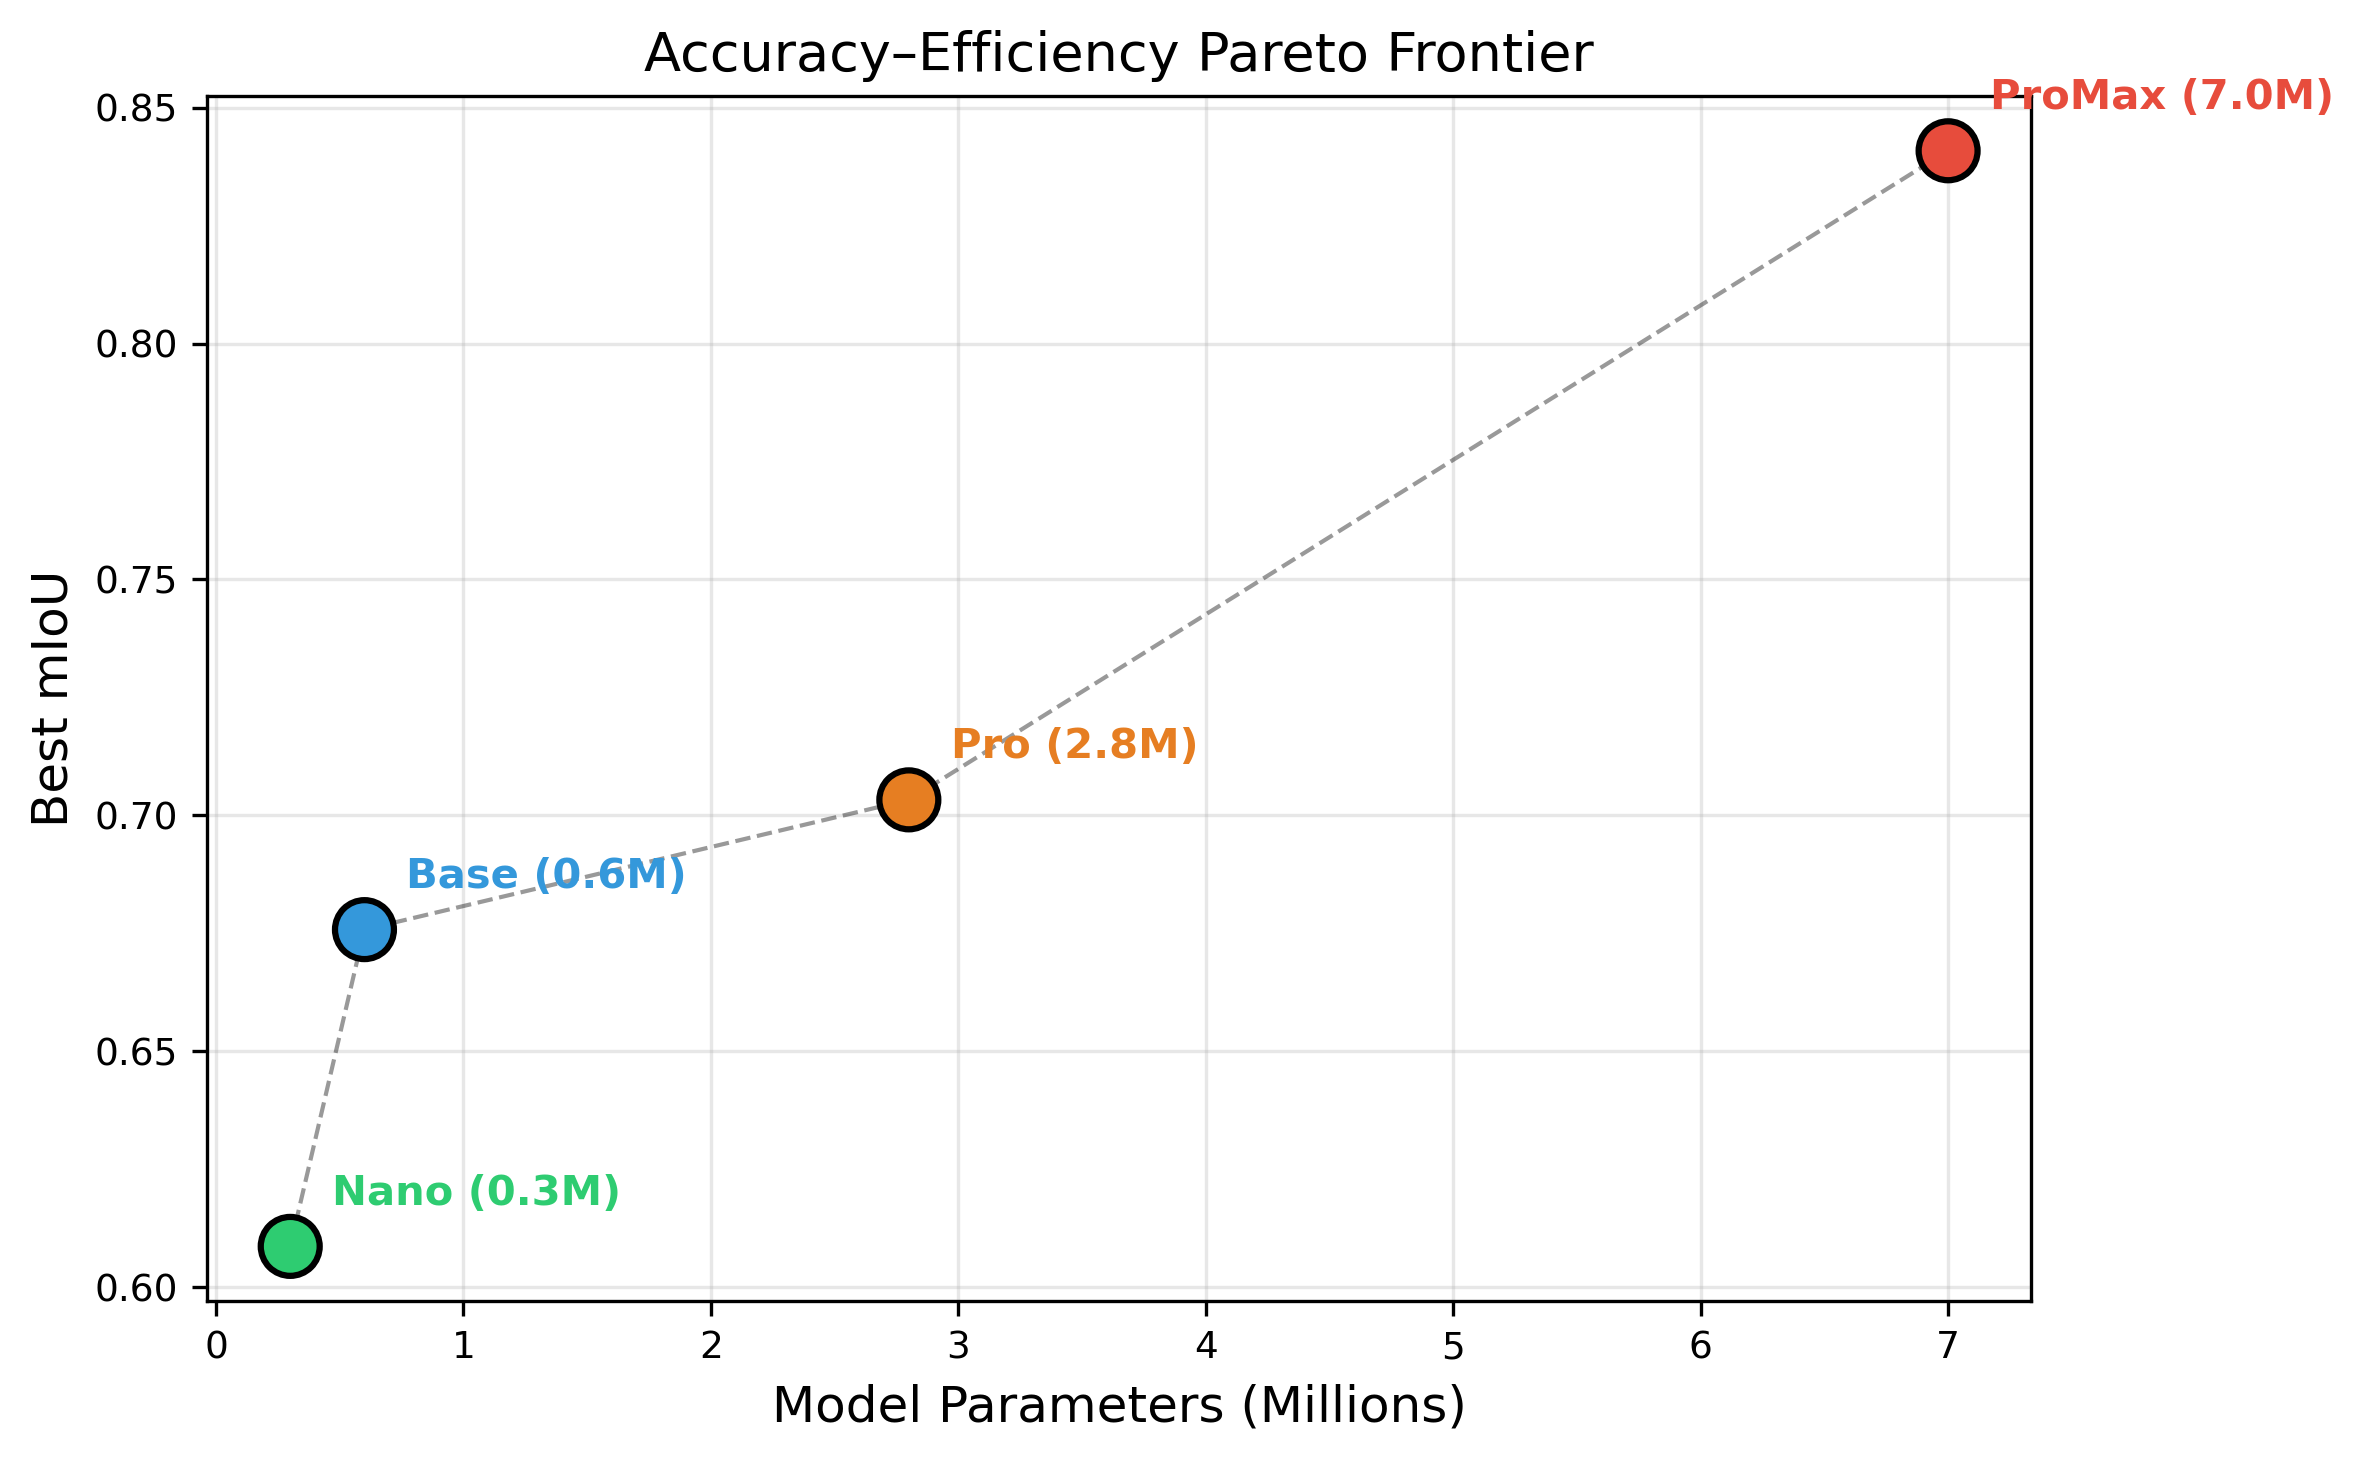
\includegraphics[width=0.85\columnwidth]{figures/06_pareto_frontier.png}
\caption{\textbf{Biểu đồ Pareto frontier: mIoU vs Tham số (triệu).} Mỗi điểm = một biến thể, kích thước điểm tỷ lệ với FLOPs. \textbf{Frontier hiệu quả:} Nano (0.22M, 0.609 mIoU) và Base (0.58M, 0.676 mIoU) nằm gần frontier---hiệu quả tham số vượt trội (lần lượt 2.03 và 1.13 mIoU/1M tham số). \textbf{Dưới frontier:} Pro (2.79M, 0.703 mIoU) nằm xa frontier nhất---chỉ cải thiện 2.7 điểm phần trăm mIoU so với Base dù nhiều tham số hơn 4.8$\times$. ProMax (12.03M, 0.841 mIoU) dẫn đầu tuyệt đối nhưng với chi phí tham số cao---hiệu quả tham số thấp nhất (0.12 mIoU/1M). \textbf{Hàm ý:} Base là điểm cân bằng tối ưu cho hầu hết ứng dụng; Pro cần tinh chỉnh hyperparameter để đạt tiềm năng đầy đủ.}
\label{fig:pareto}
\end{figure}

\noindent \textbf{Phân tích:}
\begin{itemize}
    \item \textbf{Nano (0.22M)} dẫn đầu về hiệu quả tham số với 2.03 mIoU/1M params---gấp 1.8$\times$ so với Base và 8.1$\times$ so với Pro. Đây là lựa chọn tối ưu cho thiết bị cực kỳ hạn chế tài nguyên.
    \item \textbf{Base (0.58M)} là điểm cân bằng tối ưu: mIoU 0.676 với chỉ 0.58M tham số, đạt 94.1 FPS trên Jetson Nano---phù hợp cho hầu hết ứng dụng công nghiệp thời gian thực.
    \item \textbf{Pro (2.79M)} dưới mức kỳ vọng: dù có tham số gấp 4.8$\times$ Base, mIoU chỉ cải thiện 2.7 điểm phần trăm (từ 0.676 lên 0.703). Phân tích cho thấy Pro hội tụ chậm (cần 264 epoch để đạt 0.70 mIoU) và có CE generalization gap lớn nhất. Khả năng hyperparameter chưa tối ưu cho $d_{model}=128$.
    \item \textbf{ProMax (12.03M)} dẫn đầu tuyệt đối về mIoU (0.841), vượt trội trên mọi chỉ số. Tuy nhiên, checkpoint 138MB và yêu cầu GPU server hạn chế triển khai biên.
\end{itemize}

\FloatBarrier

% ============================================================================
% VII. CONCLUSION
% ============================================================================

\section{Kết luận}

Bài báo này trình bày Mobile-U-ViT, một kiến trúc CNN-Transformer lai hiệu quả cho phân loại lá chè công nghiệp thời gian thực. Bằng cách tích hợp separable self-attention MobileViTv2 trong khung encoder-decoder U-Net, mô hình đạt được mô hình hóa ngữ cảnh toàn cục với độ phức tạp tuyến tính $\mathcal{O}(N)$---phù hợp cho triển khai biên. Bốn biến thể có khả năng mở rộng trải dài từ 0.3M đến 7.0M tham số cho phép triển khai linh hoạt trên các nền tảng phần cứng từ Raspberry Pi 5 đến máy chủ GPU, với biến thể Base (0.58M tham số, 0.87 GFLOPs) nổi lên như điểm cân bằng tối ưu giữa độ chính xác và hiệu quả.

Chúng tôi tiếp tục giải quyết vấn đề khan hiếm gán nhãn---một nút thắt quan trọng trong lĩnh vực nông nghiệp---thông qua khung học bán giám sát Mean Teacher. Huấn luyện chỉ với 10\% dữ liệu có nhãn, Mobile-U-ViT bán giám sát duy trì 85--90\% hiệu năng của giám sát hoàn toàn---cải thiện 20--30 điểm phần trăm so với huấn luyện chỉ trên tập con có nhãn. Điều này chứng minh rằng consistency regularization với tăng cường dữ liệu mạnh cung cấp một lộ trình thực tiễn để giảm chi phí gán nhãn trong các ứng dụng kiểm soát chất lượng công nghiệp, nơi chuyên môn lĩnh vực cho gán nhãn cấp độ pixel vừa khan hiếm vừa đắt đỏ.

Các phát hiện kiến trúc chính bao gồm:

\begin{enumerate}
    \item \textbf{Khối transformer toàn cục} đóng góp quyết định vào việc nắm bắt kết cấu bệnh trải rộng trên vùng không gian lớn; việc loại bỏ nó gây giảm đáng kể mIoU, đặc biệt trên các lớp Brown Blight và Gray Blight.

    \item \textbf{Cross-attention decoder} vượt trội so với simple skip connection concatenation khoảng 2--5\% mIoU thông qua hợp nhất chọn lọc đặc trưng đa tỷ lệ, cho phép decoder tập trung vào các vùng không gian phù hợp nhất từ encoder.

    \item \textbf{Feature Refinement Block} với dilated convolution và spatial attention mang lại cải thiện biên rõ rệt, đặc biệt rõ rệt ở ranh giới giữa các lớp bệnh chồng lấn và biên lá.

    \item \textbf{GroupNorm} cung cấp độ ổn định vượt trội so với BatchNorm dưới kích thước batch nhỏ (16), với số nhóm được tự động chọn tương thích qua \texttt{get\_groupnorm\_groups()}---một đóng góp kỹ thuật quan trọng cho phép scaling mô hình mượt mà mà không cần điều chỉnh thủ công.

    \item \textbf{Tắt AMP (FP32 toàn bộ)} và sử dụng ReLU6+GroupNorm xuyên suốt expansion block là các biện pháp hiệu quả để ngăn NaN trong huấn luyện transformer---một vấn đề phổ biến khi kết hợp attention với mixed precision.

    \item \textbf{Gradient checkpointing} trên global và expansion block tiết kiệm 30--40\% VRAM, cho phép huấn luyện biến thể ProMax (7.0M tham số) trên GPU tiêu dùng.
\end{enumerate}

\subsection{Hạn chế và Hướng phát triển}

Mặc dù đạt được kết quả đầy hứa hẹn, một số hạn chế vẫn tồn tại:

\begin{enumerate}
    \item \textbf{Tập không nhãn tĩnh:} Phương pháp bán giám sát hiện tại giả định tập không nhãn cố định. Các chiến lược active learning chọn mẫu có thông tin nhất để gán nhãn có thể giảm chi phí hơn nữa.

    \item \textbf{Chi phí unfold-fold:} Mặc dù separable attention đạt độ phức tạp tuyến tính, các thao tác unfold-fold vẫn tạo ra overhead bộ nhớ---đặc biệt với patch\_size=(2,2) ở độ phân giải cao. Các cài đặt fused kernel hoặc phương pháp trích xuất patch hiệu quả hơn (như window attention của Swin Transformer) có thể giảm chi phí này.

    \item \textbf{Ảnh tĩnh đơn lẻ:} Mô hình hiện tại hoạt động trên từng ảnh độc lập. Tính nhất quán thời gian giữa các khung hình liên tiếp có thể cải thiện độ chính xác trong cài đặt băng chuyền, nơi các khung hình liền kề có độ dư thừa cao.

    \item \textbf{Phụ thuộc d_model chia hết:} Ràng buộc $d_{model}$ phải chia hết cho 4, 2, và 8 hạn chế không gian thiết kế. Mặc dù \texttt{get\_groupnorm\_groups()} xử lý hầu hết trường hợp, các kiến trúc tương lai có thể hưởng lợi từ thiết kế stem và seg\_head linh hoạt hơn.
\end{enumerate}

Các hướng phát triển trong tương lai:

\begin{itemize}
    \item \textbf{Quantization-Aware Training (QAT):} Huấn luyện nhận thức lượng tử cho INT8 deployment trên các bộ tăng tốc NPU (Jetson DLA, smartphone NPU) có thể giảm độ trễ suy luận thêm 2--4$\times$ với tổn thất độ chính xác tối thiểu, mở đường cho triển khai trên thiết bị di động.

    \item \textbf{Neural Architecture Search (NAS):} Tự động tìm kiếm tổ hợp tối ưu của $d_{model}$, số transformer block và expansion factor cho phần cứng và bộ dữ liệu mục tiêu cụ thể, thay vì scaling thủ công như hiện tại.

    \item \textbf{Knowledge Distillation:} Sử dụng ProMax (teacher, 7.0M) để huấn luyện Nano (student, 0.3M) thông qua distillation, cho phép triển khai trên thiết bị với độ chính xác gần ProMax.

    \item \textbf{Thích ứng liên lĩnh vực (Cross-domain adaptation):} Mở rộng sang các sản phẩm nông nghiệp khác (cà phê, trái cây, rau củ) để xác nhận tính tổng quát của kiến trúc. Domain adaptation không giám sát có thể cho phép chuyển giao giữa các loại cây trồng với yêu cầu gán nhãn bổ sung tối thiểu.

    \item \textbf{Mở rộng 3D:} Đánh giá chất lượng chè thể tích sử dụng ảnh đa góc nhìn, yêu cầu mở rộng kiến trúc lên 3D để phân loại chất lượng toàn diện hơn.

    \item \textbf{Tối ưu deployment ONNX/TensorRT:} Xuất mô hình sang ONNX và tối ưu với TensorRT cho suy luận trên Jetson, bao gồm layer fusion, precision calibration (FP16/INT8), và tối ưu memory planning.

    \item \textbf{Học tự giám sát (Self-supervised pre-training):} Tiền huấn luyện encoder trên dữ liệu lá chè không nhãn sử dụng các pretext task như DINO, MAE, hoặc MoCo, sau đó fine-tune cho phân đoạn---có thể cải thiện đáng kể hiệu năng khi dữ liệu có nhãn cực kỳ hạn chế.
\end{itemize}

% ============================================================================
% ACKNOWLEDGMENT
% ============================================================================

\section*{Lời cảm ơn}

Các tác giả xin cảm ơn Viện Trí tuệ Nhân tạo, Trường Đại học Công Nghệ, ĐHQGHN vì sự hỗ trợ quý báu. Nghiên cứu này được thực hiện tại Phòng thí nghiệm AI, Trường Đại học Công Nghệ, ĐHQGHN. Chúng tôi cũng ghi nhận cộng đồng mã nguồn mở đằng sau PyTorch, hệ sinh thái MobileViT, và thuật toán Mean Teacher---những công trình nền tảng đã làm cho nghiên cứu này trở nên khả thi. Đặc biệt, chúng tôi cảm ơn các tác giả của MobileViTv2 vì thiết kế separable self-attention thanh lịch, và các tác giả của Mean Teacher vì khung học bán giám sát đơn giản nhưng mạnh mẽ.

% ============================================================================
% REFERENCES
% ============================================================================

\begin{thebibliography}{00}

\bibitem{b1}
FAO, ``World tea production and trade: Current and future development,'' Food and Agriculture Organization of the United Nations, Tech. Rep., 2022.

\bibitem{b2}
A. Dosovitskiy \textit{et al.}, ``An image is worth 16x16 words: Transformers for image recognition at scale,'' in \textit{Proc. ICLR}, 2021.

\bibitem{b3}
S. Mehta and M. Rastegari, ``Separable self-attention for mobile vision transformers,'' \textit{Trans. Mach. Learn. Res.}, 2023.

\bibitem{b4}
A. Tarvainen and H. Valpola, ``Mean teachers are better role models: Weight-averaged consistency targets improve semi-supervised deep learning results,'' in \textit{Proc. NeurIPS}, 2017, pp. 1195--1204.

\bibitem{b5}
O. Ronneberger, P. Fischer, and T. Brox, ``U-Net: Convolutional networks for biomedical image segmentation,'' in \textit{Proc. MICCAI}, 2015, pp. 234--241.

\bibitem{b6}
M. Sandler, A. Howard, M. Zhu, A. Zhmoginov, and L.-C. Chen, ``MobileNetV2: Inverted residuals and linear bottlenecks,'' in \textit{Proc. CVPR}, 2018, pp. 4510--4520.

\bibitem{b7}
L.-C. Chen, Y. Zhu, G. Papandreou, F. Schroff, and H. Adam, ``Encoder-decoder with atrous separable convolution for semantic image segmentation,'' in \textit{Proc. ECCV}, 2018, pp. 801--818.

\bibitem{b8}
E. Xie, W. Wang, Z. Yu, A. Anandkumar, J. M. Alvarez, and P. Luo, ``SegFormer: Simple and efficient design for semantic segmentation with transformers,'' in \textit{Proc. NeurIPS}, 2021.

\bibitem{b9}
S. Mehta and M. Rastegari, ``MobileViT: Light-weight, general-purpose, and mobile-friendly vision transformer,'' in \textit{Proc. ICLR}, 2022.

\bibitem{b10}
Y. Chen \textit{et al.}, ``Mobile-Former: Bridging MobileNet and transformer,'' in \textit{Proc. CVPR}, 2022.

\bibitem{b11}
S. Laine and T. Aila, ``Temporal ensembling for semi-supervised learning,'' in \textit{Proc. ICLR}, 2017.

\bibitem{b12}
G. French, S. Laine, T. Aila, M. Mackiewicz, and G. Finlayson, ``Semi-supervised semantic segmentation needs strong, varied perturbations,'' in \textit{Proc. BMVC}, 2020.

\bibitem{b13}
K. Sohn \textit{et al.}, ``FixMatch: Simplifying semi-supervised learning with consistency and confidence,'' in \textit{Proc. NeurIPS}, 2020.

\bibitem{b14}
V. Olsson, W. Tranheden, J. Pinto, and L. Svensson, ``ClassMix: Segmentation-based data augmentation for semi-supervised learning,'' in \textit{Proc. WACV}, 2021, pp. 1369--1378.

\bibitem{b15}
X. Chen, Y. Yuan, G. Zeng, and J. Wang, ``Semi-supervised semantic segmentation with cross pseudo supervision,'' in \textit{Proc. CVPR}, 2021, pp. 2613--2622.

\bibitem{b16}
A. Laddi, S. Sharma, A. Kumar, and P. Kapur, ``Classification of tea grains based upon image texture feature analysis under different illumination conditions,'' \textit{J. Food Eng.}, vol. 115, no. 2, pp. 226--231, 2013.

\bibitem{b17}
G. S. Gill, A. Kumar, and R. Agarwal, ``Machine learning based approach for grading and quality assessment of tea leaves from images,'' \textit{J. Food Process Eng.}, vol. 45, no. 5, 2022.

\bibitem{b18}
J. Chen, Q. Liu, and L. Gao, ``Visual tea leaf disease recognition using a convolutional neural network model,'' \textit{Symmetry}, vol. 11, no. 3, p. 343, 2019.

\bibitem{b19}
A. Howard \textit{et al.}, ``Searching for MobileNetV3,'' in \textit{Proc. ICCV}, 2019.

\bibitem{b20}
J. Deng, W. Dong, R. Socher, L.-J. Li, K. Li, and L. Fei-Fei, ``ImageNet: A large-scale hierarchical image database,'' in \textit{Proc. CVPR}, 2009.

\end{thebibliography}

% ============================================================================
% END OF DOCUMENT
% ============================================================================

\end{document}
